\chapter{Looking for \mb{\Bmumumu} decays at LHCb}
\label{chap:sel}

\textit{One of the LHCb's flagship analyses contain several muons in the final state coming from differently flavoured $B$ mesons, such as search for $B_{s}^{0}\rightarrow \mu^{+} \mu^{-}$. Despite being in this category, the search for the \Bmumumu is limited by the rareness of its occurrence as well as the different backgrounds that can mimic its signature in the detector. Moreover, presence of of the invisible neutrino in the decay induces uncertainties into the reconstruction. This chapter concentrates on data selection which reduces background contamination. Also, normalisation channel selection is discussed. In the end, a method to improve sensitivity is introduced.}



\section{Topology of the \mb{\Bmumumu} decay at LHCb}

Upon hadronisation from a $b\bar{b}$ pair, a \Bpm particle will travel around a centimetre in the laboratory frame of reference before it decays. This allows reconstruction of a primary vertex \gls{PV} and its decay vertex \gls{SV}. By joining these vertices, the direction as well as flight distance \gls{FD}, can be established. In order to infer information about the kinematic properties of \Bpm meson, the decay products are studied. All three muons are used to reconstruct the visible four-momentum. By conservation of momentum, %with respects to the direction of the flight of \Bpm,
the neutrino is assigned all missing momentum transverse to the direction of the flight of the \Bpm meson. A schematic diagram of the decay topology can be seen in~\autoref{fig:sigtopolog}.

\begin{figure}[!h]
	\centering
	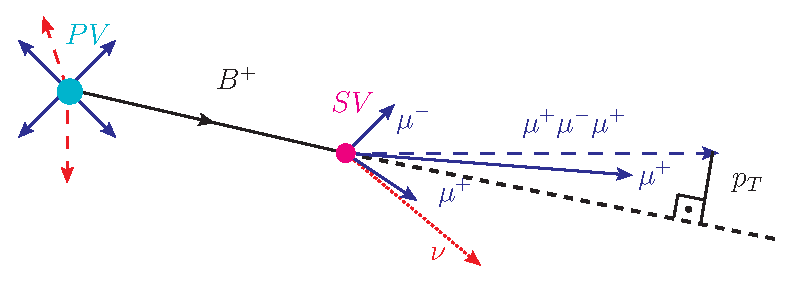
\includegraphics[width = 0.8\textwidth]{figs/sel/DecReco_fin.eps}
	\caption{Schematic view of the \Bmumumu decay. All charged particle tracks (in solid-blue) are combined into a four-vector representing the visible part of the decay (dashed-blue). Information about the invisible neutrino (dashed-red) are deduced from the conservation of momentum with respect to the direction of the flight of the \Bpm meson.}% Neglecting momentum component parallel to the direction of flight for neutrino, transverse component of momentum is given.}
	\label{fig:sigtopolog}
\end{figure}

Combining all information allows for reconstruction of the \emph{corrected mass} that plays a similar role to invariant mass in fully reconstructed decays. Invariant mass is usually used in \gls{LHCb} as the distribution from which the yield of a signal decay is determined through a fit. This particular quantity is used as it distinguishes well signal and background shapes with minimal modelling assumptions.

The \emph{Corrected mass} is defined as

\begin{equation}
	M_{corr} = \sqrt{{M}^{2} + |p^{2}_{T}|} + |p_{T}|,
\label{eq:corrm}        
\end{equation}	
where the $M^{2}$ is the invariant visible mass squared and $p^{2}_{T}$ is the missing momentum squared transverse to the direction of the $B^{+}$ meson flight. The corrected mass of the \Bpm meson will be denoted as $M_{B_{corr}}$. The $M_corr$ is equal to the true mass if the missing part of the decay has zero mass and has no momentum along the $\Bpm$ flight direction. Otherwise, $M_corr$ is below the $\Bpm$ mass.
%\begin{equation}
%M_{B_{corr}} = \sqrt{M_{\mu^{+} \mu^{-} \mu^{+}}^{2} + |p_{T}|} + |p_{T}|,
%\end{equation}	

$M_{corr}$ can be thought of as the minimal correction to the visible mass to account for the missing neutrino information. The resolution on the \textit{corrected mass} (the uncertainty of this quantity) hence becomes a critical quantity that needs to be understood. As the method of reconstruction of corrected mass relies heavily on the knowledge of the \Bpm meson flight direction, the resolution of \gls{PV} position and \gls{SV} vertex is crucial. Let $\vec{{x}}_{PV}=\{x_{PV},y_{PV},z_{PV}\}$, $\vec{{x}}_{SV}=\{x_{SV},y_{SV},z_{SV}\} $ be \gls{PV} and \gls{SV} vertex position and $\vec{p}=\{p_{x},p_{y},p_{z}\}$ be the visible trimuon momentum. Then the missing transverse momentum to the direction of the flight $p_{T}$ (momentum of the neutrino) as shown in~\cite{Egede:1694339} is


\begin{equation}
	p^{2}_{T} = \Big|\vec{p} - (\vec{{x}}_{SV}-\vec{{x}}_{PV})\frac{\vec{p} \cdot(\vec{{x}}_{SV}-\vec{{x}}_{PV})}{|(\vec{{x}}_{SV}-\vec{{x}}_{PV})|^{2}}\Big|^{2}. 
\label{eq:ptmis}
\end{equation}



In general in order to propagate error on $f(x,y,z)$, where $x,y,z$ are independent variables, the variance of $f(x,y,z)$ is given as

\begin{equation}
\begin{aligned}
	\langle f^{2}-\langle f \rangle^{2} \rangle  &=  \langle f(x+\delta x, y+\delta y, z+\delta z)^{2} - f(\langle x \rangle, \langle y \rangle, \langle z \rangle)^{2} \rangle \\
\end{aligned}
\end{equation}
Using a first order Taylor expansion of variance and rewriting it into matrix form gives

\begin{equation}
\begin{aligned}
%	\langle \frac{\partial{f}}{\partial{x}}  \frac{\partial{f}}{\partial{x}} \times \delta x^{2} + \frac{\partial{f}}{\partial{y}}  \frac{\partial{f}}{\partial{y}} \times \delta y^{2} + \frac{\partial{f}}{\partial{z}}  \frac{\partial{f}}{\partial{z}} \times \delta z^{2} + \sum_{i,j=1..3, i \neq j} \partial_{d_{i}} \partial_{d_{i}}  \frac{\partial{f}}{\partial{x}} \frac{\partial{f}}{\partial{y}} \rangle \\ 
%        = 
       \begin{bmatrix}
		\frac{\partial{f}}{\partial{x}} & \frac{\partial{f}}{\partial{y}} & \frac{\partial{f}}{\partial{z}} \\
       \end{bmatrix}
       \begin{bmatrix}
	       {\delta x}^{2} & \delta x \delta y & \delta x \delta z  \\ 
	        \delta y \delta x & {\delta y}^{2} & \delta y \delta z  \\
	        \delta z \delta x & \delta z \delta y & {\delta z}^{2}  \\
       \end{bmatrix}
       \begin{bmatrix}
		\frac{\partial{f}}{\partial{x}} \\ \frac{\partial{f}}{\partial{y}} \\\frac{\partial{f}}{\partial{z}}. \\
       \end{bmatrix}
\end{aligned}
\end{equation}
In this formalism let $f$ is the \emph{corrected mass} and $x,y,z$ are variables on which \emph{corrected mass} depends. Using~\autoref{eq:corrm}, these independent variables are visible mass four-vector, $p_{3\mu}=\{E,p_{x},p_{y},p_{z}\}$, and missing $p_{T}$ (defined in~\autoref{eq:ptmis}), which in turn depends on $\vec{p}$, $\vec{x_{PV}}$ and $\vec{x_{SV}}$.

With $x=\vec{{x}}_{PV}$, $y=\vec{{x}}_{SV}$, $z=p_{3\mu}$ and \rm{COV} being the covariance matrix, the error (square root of variance) on the \emph{corrected mass}, $\delta_{corrm}$ is
%\begin{equation}
%\begin{aligned}
%       \nabla^{T}_{x_{PV}} \rm{C_{x_{PV}}} \nabla_{x_{PV}} + \nabla^{T}_{x_{SV}} \rm{C_{x_{SV}}} \nabla_{x_{SV}} + \nabla^{T}_{p} \rm{C_{p}} \nabla_{p}
%\end{aligned}
%\end{equation}
%
%where \rm{C} is the covariance matrix.
%
%In conclusion in order to calculate error on \textit{corrected mass}, $\delta_{corrm}$


\begin{equation}
\begin{aligned}
	\delta_{corrm} = \sqrt{ \langle f^{2}-\langle f \rangle^{2} \rangle} = \sqrt{\nabla^{T}_{x_{PV}} \mathrm{COV}_{x_{PV}} \nabla_{x_{PV}} + \nabla^{T}_{x_{SV}} \mathrm{COV}_{x_{SV}} \nabla_{x_{SV}} + \nabla^{T}_{p_{3\mu}} \mathrm{COV}_{p_{3\mu}} \nabla_{p_{3\mu}}}. 
\end{aligned}
\end{equation}
It was shown in~\cite{Egede:1694339} that the $\delta_{corrm}$ is mostly dominated by vertex position terms.
%which can be calculated analytically (method used for all the plots) or using numerical approximation of first derivative of \textit{finite differences}.

\section{Sources of Backgrounds}
\label{bkgquick}
The largest background that looks similar to signal comes from \textit{cascade decays}, where the semileptonic $b \rightarrow c \rightarrow s$ or $\bar{b} \rightarrow \bar{c} \rightarrow \bar{s}$ transitions occur. A typical example of this type of background in hadronic terms is $B^{+} \rightarrow (\bar{D}^{0} \rightarrow (K^{+} \rightarrow \mu^{-} \nu)\ \mu^{+} \nu$), where the $K^{+}$ meson is subsequently misidentified as muon. Because the $K^{+}$ meson is misidentified as a muon, this type of background is denoted as misID background.

All background sources that contain at least one misidentified particle are categorized as misID. If the sign of the misidentified particle agrees with the sign of the mother \Bpm, it belongs to the same sign misID background (\textit{SS misID}) background. In the event where a particle with the opposite sign to the mother $\Bpm$ meson is misidentified, this background will be referred to as (\textit{OS misID}) background. \textit{OS misID} background is expected to have a smaller rate as the misidentified particle would have to proceed via decays with additional particles.

As the hadronisation of a $b\bar{b}$ pair leads to the creation of two-$b$ hadrons, each with they own decay chain, it is possible to mix up the decay products of the two to create a single fake signal candidate. This type of background is known as combinatorial background.

Then presence of a neutrino in a final state introduces uncertainty regarding the information of the fourth decay product. If some of the tracks of the decays are not reconstructed, either because they are neutral, or they are charged but with too low momentum to be found by the tracking algorithm, it means that the missing information may be attributed to the neutrino. \textit{Missing tracks} will hence create partially reconstructed background. Some of the most dangerous are ${B^{+} \rightarrow D \mu^{+} \nu}$ type partially reconstructed backgrounds, where $D^0 \rightarrow K^- \pi^+ \mu^{+} \mu^{-}$.

Decays that proceed via hadronic resonances such as $B^{+} \rightarrow \rho/\omega \mu^{+} \nu$, followed by $\rho/\omega \rightarrow \mu^{+} \mu^{-}$ are part of signal as mentioned in~\autoref{mydecay}.

Detailed information concerning these types of backgrounds are discussed in~\autoref{chap:back}.

\section{Analysis strategy}
\label{Strategy}

The analysis of the $\Bmumumu$ decay is divided into several different parts; signal selection, optimisation, normalisation, fitting and limit setting. Throughout this document, charge conjugates of the decays are assumed unless stated otherwise. Results presented are based on the analysis of the full 3 fb$^{-1}$ Run \Rn{1} dataset as well $\approx$ 1.7 fb$^{-1}$ Run \Rn{2} data from 2016. Data from 2015 is not used due to the very high $p_{T}$ threshold for the muon triggers used during that year, resulting in a very low signal efficiency. Additionally the search will be conducted in a particular $minq$ = $\sqrt{min(q^{2}(\mu_{1}^{+},\mu^{-}), q^2(\mu^{-},\mu_{2}^{+}))}$ region, described in~\autoref{qsqchoice}.  


To perform the search for $\Bmumumu$, a specific preselection was applied to form potential signal candidates as described in~\autoref{preselection}. A simulation sample that mimics the decay of the $\Bmumumu$ was created, as mentioned in~\autoref{simulation}. This simulation together with the background proxies discussed in~\autoref{chap:back} are used to further develop discriminating selection that would maximize the signal to background ratio. Most of the rest of this chapter is dedicated to this discriminating selection. For more details about signal simulation samples see~\autoref{SimulationSamples}.


After all the selection, the $\Bmumumu$ decays are normalised to the $\bjpsimumuk$ decays, where the selection for the normalisation channel, detailed in~\autoref{nchannel}, is kept as similar as possible to that of the signal channel to minimize the amount of systematics on the resulting relative efficiencies between these two channels. The relative efficencies are computed in~\autoref{EfficiencyRatio}. The fit to $\bjpsimumuk$ data is described in~\autoref{normfit}. The relative efficiencies, results of the normalisation channel fit and the branching fraction of \bjpsimumuk are used to parametrise the expected signal yield, as described in~\autoref{sigpara}.



Throughout the analysis there was a blinding procedure put in place for this search in order not to bias the result. The signal region $4500{\mevcc}<M_{\rm{B_{corr}}}<{5500\mevcc}$ was blinded until full strategy and sensitivity was evaluated. The signal dataset corresponding to this selection is known as \textbf{blinded signal dataset}. After unblinding, data with full mass spectrum was obtained and is known as \textbf{full signal dataset}.%  Hence in all blinded fits only data in regions $4000{\mevcc}<M_{\rm{B_{corr}}}<{4500\mevcc}$ and $5500{\mevcc}<M_{\rm{B_{corr}}}<{7000\mevcc}$ are used.



In~\autoref{fitsens}, two fitting strategies for the signal data are described. One is more sensitive than another, where the fitting strategy that provides the best sensitivity makes use of simultaneous fit to two bins of resolution, increasing signal separation from background. More information about this split can be found in~\autoref{split}. Both fitting strategies were applied on blinded signal datasets in order to compute the expected exclusion limit on the branching fraction, shown in~\autoref{sensitivity}. Systematic uncertainties that are affecting this measurement are presented in~\autoref{systematics}.


Upon unblinding, no significant signal was observed and stringent limit $\mathcal{B}(\Bmumumu) < 1.4\times 10^{-8}$ at $95\%$ confidence level was set using $CL_{s}$ method with simultaneous fit. All information about the result as well as the implication can be found in~\autoref{chap:Results}.% This result does not confirm the prediction for the decay branching fraction\cite{Danilina:2017bcn}\cite{Danilina:2018uzr}, where $\mathcal{B}(\Bmumumu) \approx 1.3\times 10^{-7}$.


%In summary, the aim of the analysis is to fit corrected mass of $B^{+}$ in bins of fractional corrected mass error. This is the fitting strategy that provides the best sensitivity (described in detail in~\autoref{split}) but the motivation for this particular strategy is that the signal data is split into two bins of resolution, increasing signal separation from background.







\section{Signal Simulation Samples}
\label{SimulationSamples}
%\subsection{Data Samples}

%Results presented in this thesis are based on the analysis of the full 3 fb$^{-1}$ Run \Rn{1} dataset at $\sqrt{s}={7},{8}$ \tev and 1.7 fb$^{-1}$ Run \Rn{2} data at $\sqrt{s}=13$\tev.

%\subsection{Simulation Samples}
%\label{SimulationSamples}
For signal simulation three different decay models are used for different purposes summarized in~\autoref{tab:MCPPass}. The physics rationale behind these models was discussed in~\autoref{simulation}.

\begin{table}[h!]
	\begin{center}
		\begin{tabular}{l l l l l l}
                       \toprule
			Channel & Year & Pythia  & EVTGEN & Size & Stage \\ \hline
			 \multicolumn{6}{c}{Simulation used for fitting mass shapes} \\ \hline
			$B^{+} \rightarrow \mu^{+} \mu^{-} \mu^{+} \nu$ & 2012 & Pythia 6.4\cite{pythia6} & PHSP & 0.5$\rm{M}$ & \textit{generator-level+detector}\\
			$B^{+} \rightarrow \mu^{+} \mu^{-} \mu^{+} \nu$ & 2012 & Pythia 8.1\cite{pythia8} & PHSP & 0.5$\rm{M}$ & \textit{generator-level+detector}\\
			$B^{+} \rightarrow \mu^{+} \mu^{-} \mu^{+} \nu$ & 2012 & Pythia 6.4\cite{pythia6} & INSP & 0.5$\rm{M}$ & \textit{generator-level+detector}\\
			$B^{+} \rightarrow \mu^{+} \mu^{-} \mu^{+} \nu$ & 2012 & Pythia 8.1\cite{pythia8} & INSP & 0.5$\rm{M}$ & \textit{generator-level+detector}\\
			$B^{+} \rightarrow \mu^{+} \mu^{-} \mu^{+} \nu$ & 2016 & Pythia 8.1\cite{pythia8} & INSP & 1.0$\rm{M}$ & \textit{generator-level+detector}\\ \hline
			 \multicolumn{6}{c}{Simulation used for evaluating \textit{generator-level} efficiencies} \\ \hline
			$B^{+} \rightarrow \mu^{+} \mu^{-} \mu^{+} \nu$ & 2012 & Pythia 6.4\cite{pythia6} & PHSP & 25000 & \textit{generator-level}\\ %using only for comaprison pythia 6
			$B^{+} \rightarrow \mu^{+} \mu^{-} \mu^{+} \nu$ & 2012 & Pythia 6.4\cite{pythia6} & INSP & 25000 & \textit{generator-level}\\
			$B^{+} \rightarrow \mu^{+} \mu^{-} \mu^{+} \nu$ & 2012 & Pythia 8.1\cite{pythia8} & INSP & 25000 & \textit{generator-level}\\ \hline

                         \multicolumn{6}{c}{Simulation used for cross-checking of $minq$ selection} \\ \hline 

			$B^{+} \rightarrow \mu^{+} \mu^{-} \mu^{+} \nu$ & 2012 & Pythia 6.4\cite{pythia6} & NIKI & 25000 & \textit{generator-level}\\ %\hline
			%			\hline
%			$B^{+} \rightarrow J/\psi K^{+}$ & 2011 & Pythia6\cite{pythia6} & /Sim08c/Digi13/Trig0x40760037/Reco14a/Stripping20r1NoPrescalingFlagged \\
%			$B^{+} \rightarrow J/\psi K^{+}$ & 2011 & Pythia8\cite{pythia8} & /Sim08c/Digi13/Trig0x40760037/Reco14a/Stripping20r1NoPrescalingFlagged \\
%			$B^{+} \rightarrow J/\psi K^{+}$ & 2012 & Pythia6\cite{pythia6} & /Sim08h/Digi13/Trig0x409f0045/Reco14c/Stripping20NoPrescalingFlagged \\
%			$B^{+} \rightarrow J/\psi K^{+}$ & 2012 & Pythia8\cite{pythia8} & /Sim08h/Digi13/Trig0x409f0045/Reco14c/Stripping20NoPrescalingFlagged \\
%			%$B^{+} \rightarrow J/\psi K^{+}$ & 2015 & Pythia8 & /Sim09a/Trig0x411400a2/Reco15a/Turbo02/Stripping24NoPrescalingFlagged \\
%			$B^{+} \rightarrow J/\psi K^{+}$ & 2016 & Pythia8\cite{pythia8} & /Sim09b/Trig0x6138160F/Reco16/Turbo03/Stripping26NoPrescalingFlagged \\
%			\hline
%			$B^{+} \rightarrow J/\psi \pi^{+}$ & 2012 & Pythia6\cite{pythia6} & /Sim08a/Digi13/Trig0x409f0045/Reco14a/Stripping20NoPrescalingFlagged \\
%			$B^{+} \rightarrow J/\psi \pi^{+}$ & 2012 & Pythia8\cite{pythia8} & /Sim08a/Digi13/Trig0x409f0045/Reco14a/Stripping20NoPrescalingFlagged \\
%
%			\hline
%			$B^{0} \rightarrow J/\psi K^{*}$ & 2011 & Pythia8 & /Sim08f/Digi13/Trig0x40760037/Reco14a/Stripping20r1NoPrescalingFlagged\\
%			$B^{0} \rightarrow J/\psi K^{*}$ & 2012 & Pythia8 & /Sim08f/Digi13/Trig0x409f0045/Reco14a/Stripping20NoPrescalingFlagged\\
%			$B^{0} \rightarrow J/\psi K^{*}$ & 2016 & Pythia8 & /Sim09b/Trig0x6138160F/Reco16/Turbo03/Stripping26NoPrescalingFlagged\\
%			\hline
%			PartReco & 2012 & Pythia8 & /Sim08g/Digi13/Trig0x409f0045/Reco14a/Stripping20NoPrescalingFlagged  \\
			\bottomrule
		\end{tabular}
	\end{center}
	\caption{Summary of signal simulation samples used in this analysis with different decay models. In all cases, the daughters of the \Bpm meson are required to be within the \gls{LHCb} acceptance. All of these samples are mixture under two magnetic polarity conditions.}
	\label{tab:MCPPass}
\end{table}


The \textit{INSP} model is used as default model for mass fit shapes and efficiency calculations. The \textit{PHSP} is used for alternative efficiency calculations. Finally \textit{NIKI} model is mainly used for validation purposes.
%\mybox{Sally: move it to theory and check ulrik's comment} In order to produce simulation with a decay model which is more representative of the spin structure involved, the following strategy is adapted. In this simulation approach, the decay proceeds as follows: \Bpm decays into \Wpm and a pair of opposite sign muons and then \Wp is decayed to $\mu^{+} \nu$. \textit{BTOSLLBALL} model\cite{Ali:1999mm}, traditionally used for $\B \rightarrow (K,K^{*}) l^{+} l^{-}$ decay, with the form factor calculations can be used to simulate $\Bpm \rightarrow \Wpm l^{+} l^{-}$ decay. After that, \Wp is decayed to $\mu^{+} \nu$ using \textit{PHSP}. For semileptonic $b \rightarrow s l^{+} l^{-}$ transitions, there is a characteristic photon pole for low $q(\mu^{+},\mu^{-})$, invariant mass of the opposite muon pair, and flat distribution for $K^{*}(\mu^{+}, \nu_{\mu}) $, invariant mass of the muon and neutrino pair. In order to achieve this, a new pseudo-particle is introduced to EVTGEN with specific properties, $K^{*}(\mu^{+}, \nu_{\mu})$, and the best output can be seen to be for a particle $K^{*}(\mu^{+}, \nu_{\mu})$ with mass to be set to $0.1 \text{GeV/c}^{2}$, and width, corresponding to $\tau= 1.3\times10^{-17}$ nanoseconds as can be seen in~\autoref{fig:mcgeneration}. This procedure was also applied for the charge conjugate case. 

%This model is denoted as \textit{INSP} and is used as default in mass fits and efficiency calculations.
%
%
%\begin{figure}[h!]
%\centering
%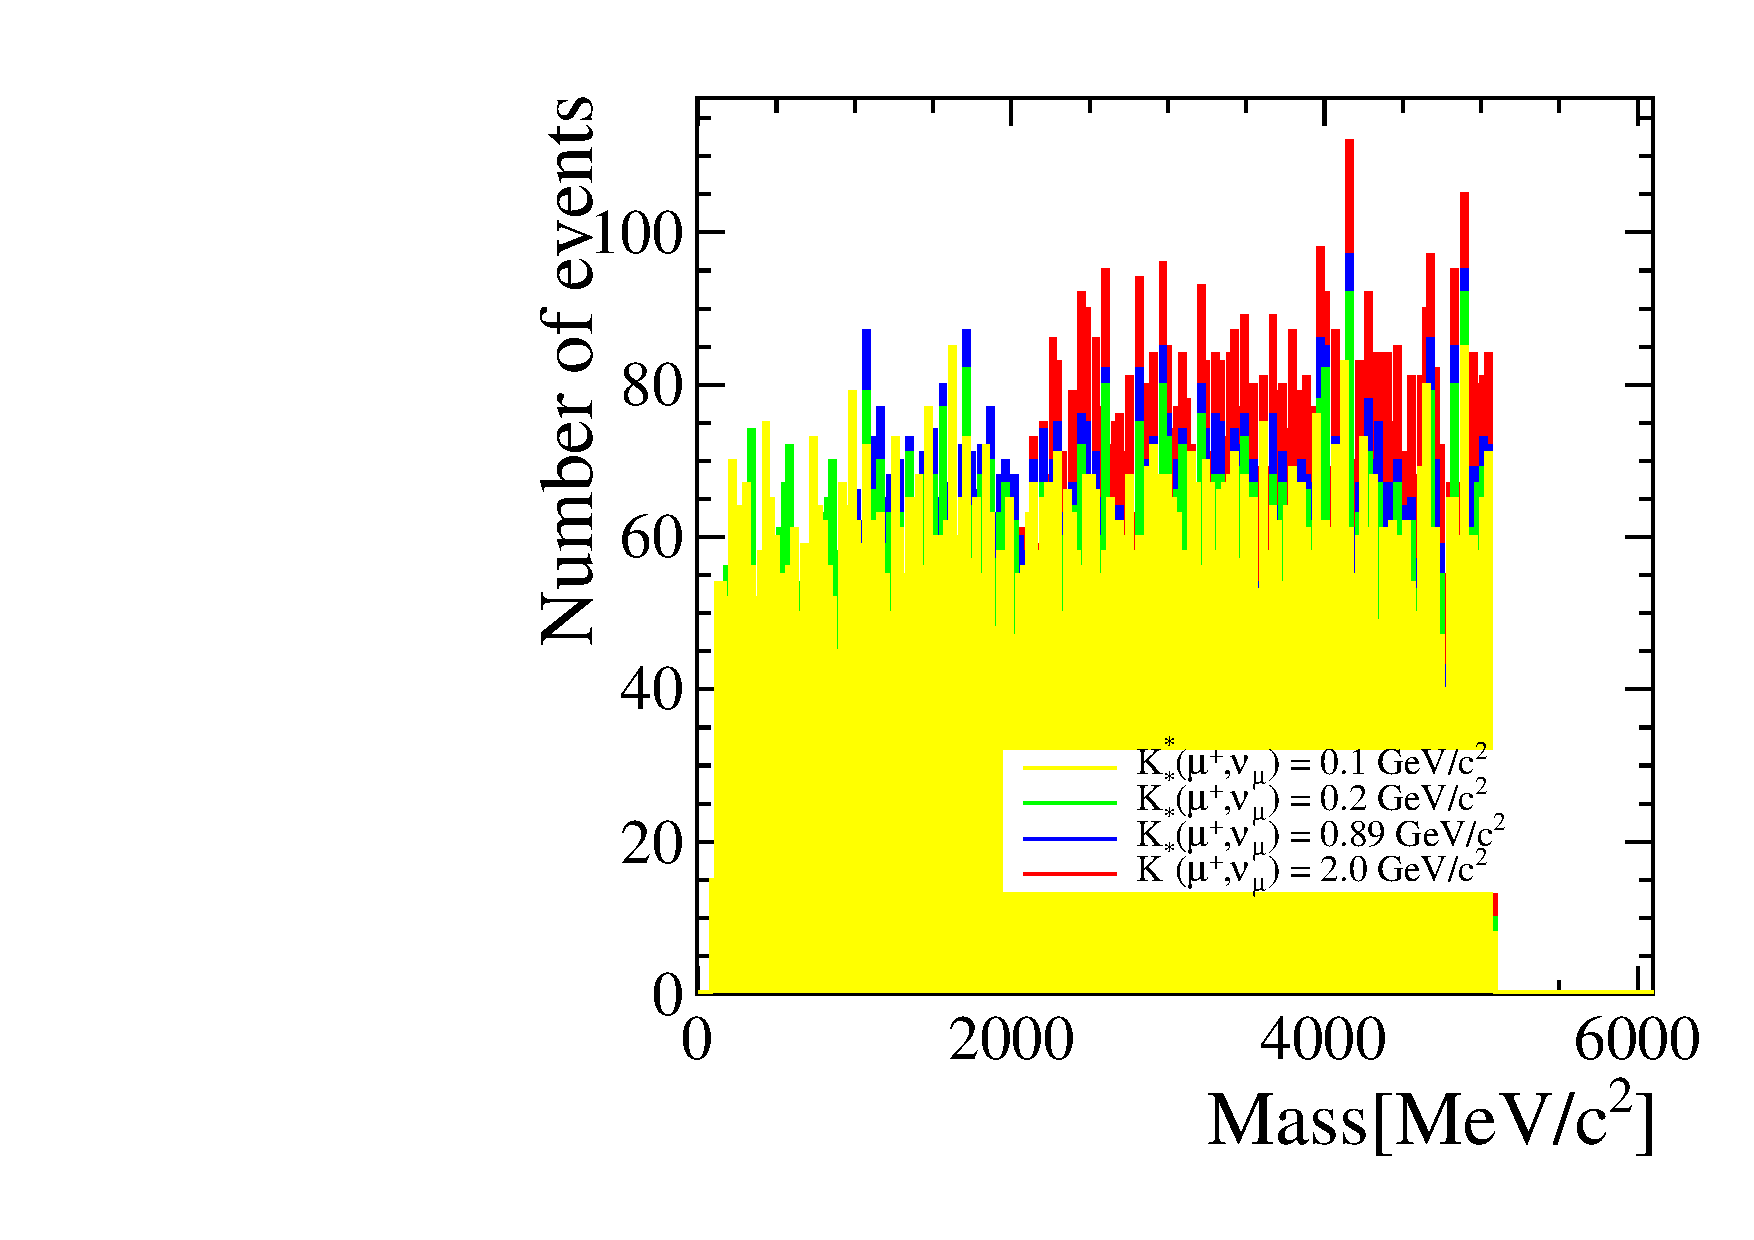
\includegraphics[width=0.5\linewidth]{./sel/reporttry_new}\put(-70,133){(a)}
%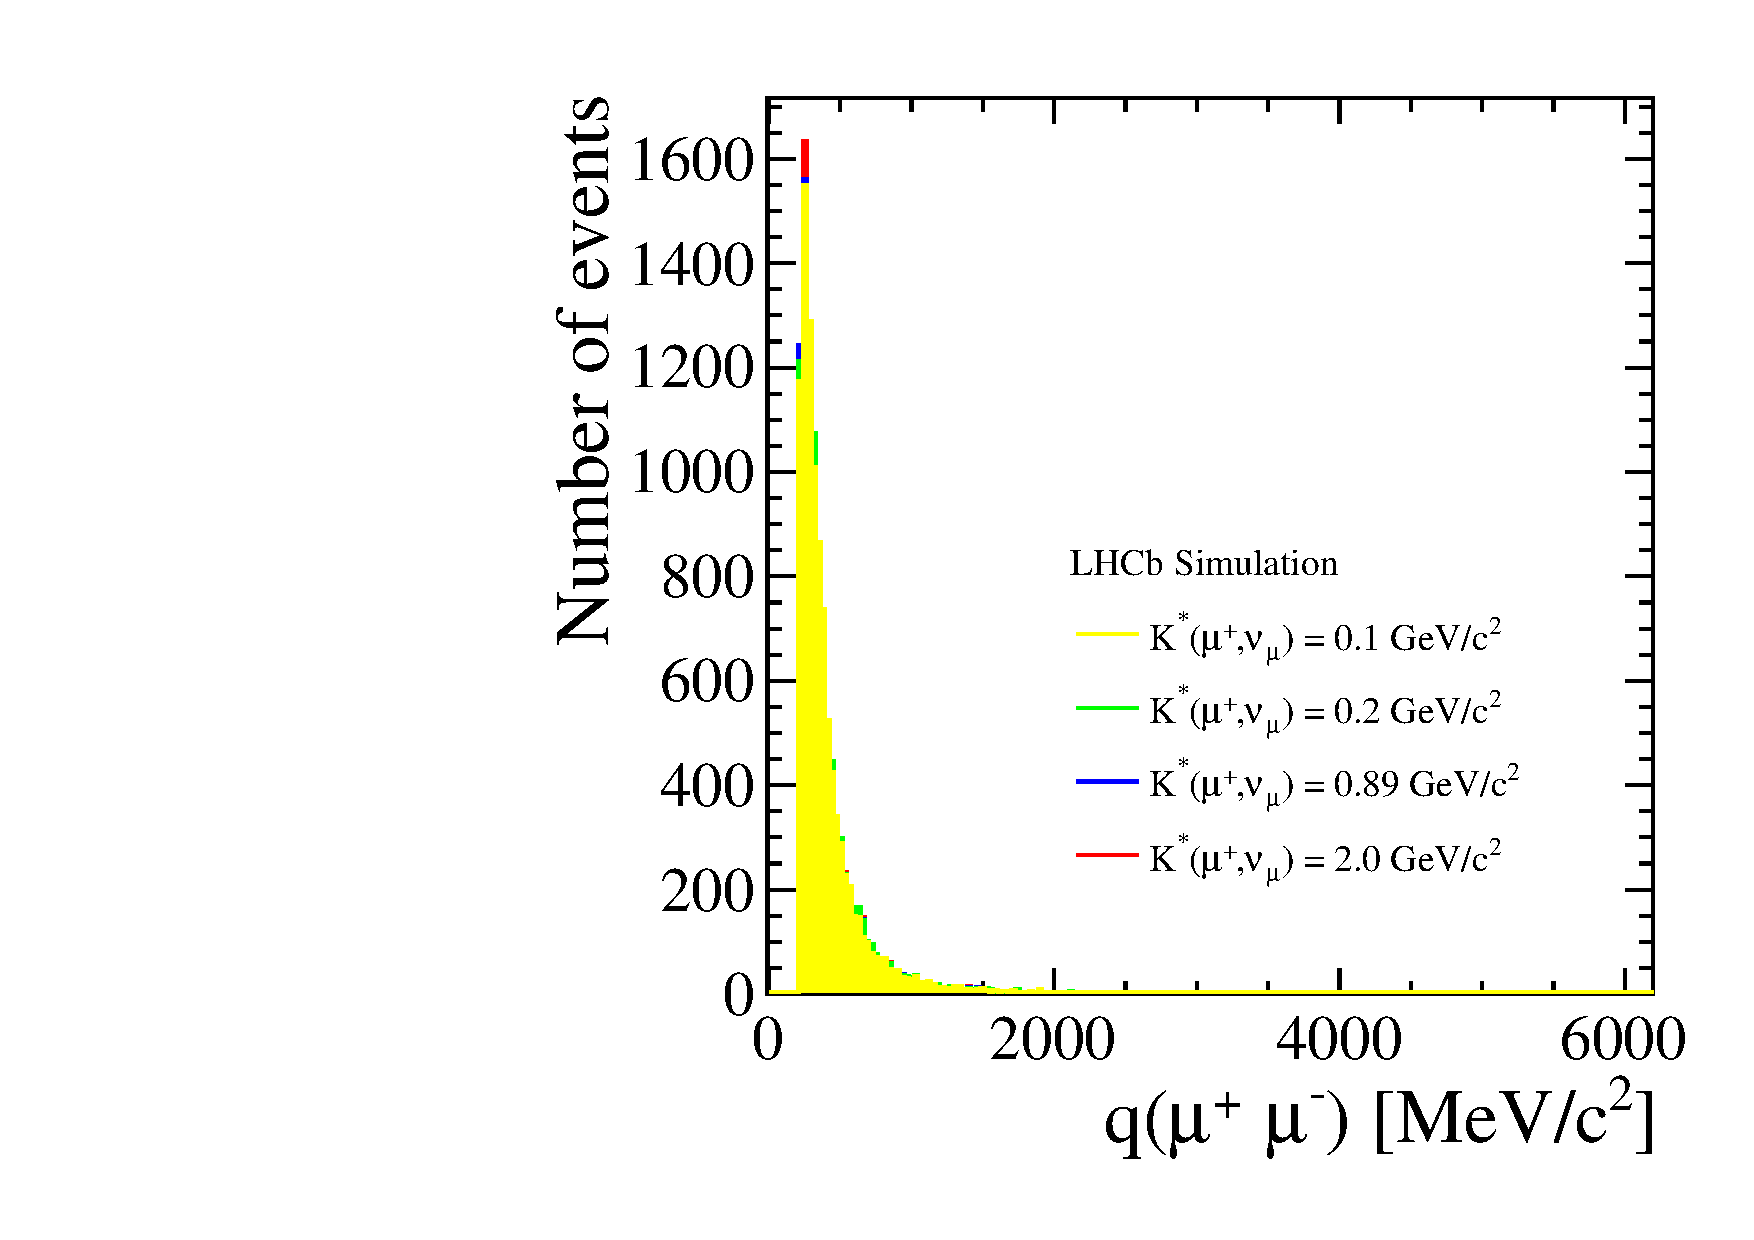
\includegraphics[width=0.5\linewidth]{./sel/reporttrialqpres_new}\put(-50,133){(b)}
%\caption{Distributions for signal MC in using Pythia 6.4 \cite{pythia6} conditions. (a) $K^{*}(\mu^{+}, \nu_{\mu})$ (b) $q(\mu^{+},\mu^{-})$ distributions under different $K^{*}$ mass hypotheses. The most flat distribution in $K^{*}(\mu^{+}, \nu_{\mu})$ is plotted in yellow.}
%\label{fig:mcgeneration}
%%\vspace*{-1.0cm}
%\end{figure}


%Finally, exclusively for this decay, a new decay model \textit{B2MuMuMuNu} was added to EVTGEN, based on work performed by theorists Anna Danilina and  Nikola Nikitin\cite{Danilina:2018uzr}. This model denoted as \textit{NIKI}, is used mainly for validation purposes. 


\section{Preselection}% for \Bmumumu}
\label{preselection}

In order to fit within the LHCb computing model, an initial set of selection criteria is applied during the data processing known as \textit{stripping}. Each of the criteria are discussed below and a summary can be found in~\autoref{tab:stripcutsB}.

%Set of initial identification for signal \Bmumumu summarized in~\autoref{tab:stripcutsB}, also known as \textit{stripping} selection was develloped in order to improve signal to background ratio. 

Firstly, all three muon tracks are required to have a significant \gls{IP} with respect to the primary vertex. Minimum Impact Parameter $\chi^{2}$, (\gls{minipchi2}), gives the minimum significance of a particles's trajectory to the primary vertex. Hence by requiring \gls{minipchi2}$>9$ for muons is consistent with the hypothesis that the muon is $3\sigma$ away from the primary vertex and hence can be well differentiated. In addition, the change in the $\chisq$ if \gls{PV} and \gls{SV} vertices are fitted separately as opposed to common vertex fit, \gls{fdchi2}, suppresses prompt backgrounds. 

Each muon track is required to have good track $\chi^{2}$ per number of degrees of freedom of the fit (\texttt{ndof}), (\gls{trackchi2ndof}), as well as low \gls{pgh2}. This removes spurious tracks as well as tracks with low quality.

Each muon candidate is also identified with initial basic \gls{PID} variables. Firstly muons are chosen due to their signature in the muons stations with the binary \texttt{isMuon} decision. Secondly, muon candidates are chosen such that it is more likely that the candidate is a muon than a pion or kaon using global DLLmu variables defined in~\autoref{muonID}. This reduces the background from misidentified muons.

In order to only select events which are compatible with the three muons originating from the same point in the space, (\gls{vertexchi2ndof}), the $\chi^{2}$ of the trimuon vertex per degree of freedom fit is required to be small. This decreases the contamination from \textit{cascade decays} where the particle with the $c$ quark content from $b \rightarrow \underline{c} \rightarrow s$, such as $D$, would have non-negligible lifetime leading to higher \gls{vertexchi2ndof}. 

Requirement that \Bp direction points in the same direction as the line from \gls{PV} to \gls{SV} is done by making sure that \gls{DIRA}, angle between the two vectors, is close to unity. This translates into a well reconstructed event, which minimizes combinatorial background, where the random track makes this pointing worse. The missing neutrino Putting bounds on the mass window, whether it is \textit{visible} or \textit{corrected} mass, also suppresses combinatorial events. % This is because of on average higher momentum combinatorial muon.  


\begin{table}[H]
\begin{center}
\begin{tabular}{l c l }
    \toprule
     Candidate & Stripping Selection \\ \hline

	muon & \gls{minipchi2} $> 9$ &  \rdelim\}{3}{1cm}[\ track] \\
	muon & $p_{T} >$ 0 \\
	muon & \gls{trackchi2ndof}$ < 3$ \\

	
	muon & DLLmu $> 0$  & \rdelim\}{3}{1cm}[\ \gls{PID}] \\
	muon & $\rm{DLLmu}-\rm{DLLK} > 0$ \\
	muon &  \texttt{isMuon==true} \\ \hline
	
	combination & \gls{DIRA} $> 0.999$ \\
        combination & $p_{T} >$ 2000 \mev\\
	combination & \gls{fdchi2} $> 50$\\
	combination & \gls{vertexchi2ndof} $< 4$ \\
	combination & $0\ \mevcc\ <\ M_B\ <\ 7500\ \mevcc$ \\
	combination & $2500\ \mevcc\ <\ M_{B_{corr}}\ <\ 10000\ \mevcc $\\ \bottomrule
     \end{tabular}

\end{center}
	\caption{Selection of events based on muon and the $B^{+}$ candidate requirements. \textit{Stripping selection} for the signal decay $B^{+} \rightarrow \mu^{+} \mu^{-} \mu^{+} \nu_\mu$ is the same for both Run1 and 2016 data.}
\label{tab:stripcutsB}
\end{table}

\section{Trigger Selection}
In order to obtain triggered data, $B^{+} \rightarrow \mu^{+} \mu^{-} \mu^{+} \nu_\mu$ candidates are required to pass a certain set of trigger decisions at \gls{L0}, \gls{HLT1} and \gls{HLT2} levels summarized in~\autoref{tab:triggersel}. It can be noted that the decision is applied at the mother \Bpm level. In particular, positive \texttt{Bplus$\_$L0MuonDecision$\_$TOS} decision means that one of the muons from \Bpm in an event triggered $\texttt{L0Muon}$.

\begin{table}[h!]
\begin{center}
	\begin{tabular}{ l l}\toprule%l | l | }
Trigger Selection  \\ %& 2011 & 2012 & 2016 \\
\hline
		\texttt{Bplus$\_$L0MuonDecision$\_$TOS} \\ %& 0.915 & 0.895 & 0.74 \\
\hline
		\texttt{Bplus$\_$Hlt1TrackMuonDecision$\_$TOS} \\% & 0.874 & 0.929 & 0.931 \\
%Or of HLT2 lines below & 0.986 & 0.987 & 0.996  \\
\hline
		\texttt{Bplus$\_$Hlt2TopoMu2BodyBBDTDecision$\_$TOS} & \rdelim\}{4}{1cm}[\ OR]\\ % & 0.859 & 0.892 & 0.94* \\
		\texttt{Bplus$\_$Hlt2TopoMu3BodyBBDTDecision$\_$TOS} \\ % & 0.677 & 0.76 & 0.886* \\
		\texttt{Bplus$\_$Hlt2DiMuonDetachedDecision$\_$TOS} \\ % & 0.809 & 0.769 & 0.988 \\
		\texttt{Bplus$\_$Hlt2DiMuonDetachedHeavyDecision$\_$TOS} \\ % & 0.94 & 0.929 & 0.99 \\
\bottomrule
\end{tabular}
\end{center}
	\caption{Trigger selection applied on both signal and normalisation samples.}
	\label{tab:triggersel}
\end{table}

As discussed in~\autoref{triggerchap} \texttt{L0MuonDecision} decides on whether an event is accepted depending on the $p_{T}$ of a muon and the number of hits in the \gls{SPD}. Run \Rn{1} can be split into 2011 and 2012 conditions where, in 2011 the most used threshold for positive decision is 1.48 \gevc \cite{Aaij:2012me} and 1.76 \gevc \cite{Albrecht:2013fba}. Run \Rn{1} \gls{SPD} rate only accepts events below 600. In Run \Rn{2}, the trigger thresholds varied more but the most representative acceptance for muon $p_{T}$ was above 1.85 \gevc with \gls{SPD} multiplicity below 450.

\texttt{Hlt1TrackMuonDecision} accepts events where at least one identified muon muon has to pass thresholds on \gls{ipchi2}, $p_{T}$ and $p$. This favours muons arising from $b$- and $c$-hadron decays. There has to be at least one muon (\texttt{isMuon==true}) in its final state with certain kinematic thresholds on $p$ and $p_{T}$. For example, in 2011 the identified muons that triggered positive decision had to have $p$ above 8 \gevc \cite{Aaij:2012me}.

At \gls{HLT2} level, the candidates are required to pass through at least one of the four decisions. \texttt{Hlt2TopoMu[2,3]BodyBBDTDecision} belong to the \textit{topological triggers} category with an extra requirement of a particle in a candidate being idendified by \texttt{isMuon} decision. \texttt{Hlt2DiMuonDetachedDecision} and \texttt{Hlt2DiMuonDetachedHeavyDecision} reconstruct decays with two muons in a final state. The two lines differ in that they are optimised for heavy and light dimuon pairs respectively. For example, \texttt{Hlt2DiMuonDetachedDecision} accepts events with dimuon $p_{T}$ above 1.5 \gevc and with mass above 1 \gevcc, whereas  \texttt{Hlt2DiMuonDetachedHeavyDecision} accepts dimuon pairs with any $p_{T}$ but above 2.95 \gevcc in mass. The reason why these lines are called detached are because individual muons are required to have high \gls{ipchi2}.

\section{\mb{q^{2}} Selection}
\label{qsqchoice}
In the \Bmumumu decay, two pairs of opposite sign muons can be formed, namely $q^2(\mu_1,\mu_2)$ and $q^2(\mu_2,\mu_3)$ where $\mu_1=\mu^{+} , \mu_2=\mu^{-}, \mu_3=\mu^{+} $.
From the two invariant mass squared pairs one can define, $minq^2 = min[q^{2}(\mu_1,\mu_2), q^2(\mu_2,\mu_3)]$ and $maxq^{2} = max[q^{2}(\mu_1,\mu_2), q^2(\mu_2,\mu_3)]$. This measurement is made in region where $minq=\sqrt{minq^{2}}<980$ \mevcc for two reasons: most of the contributions to the amplitude of the decay is below this value and combinatorial background is greatly reduced if $minq<1\gevcc$, see~\autoref{fig:qsqsel}.

In order to remove backgrounds that proceed via resonant $J/\psi$ and $\Psi(2S)$ contributions, vetoes in invariant mass are placed in the corresponding regions, see~\autoref{tab:vetoes} for more details.

\begin{figure}[h!]
\centering
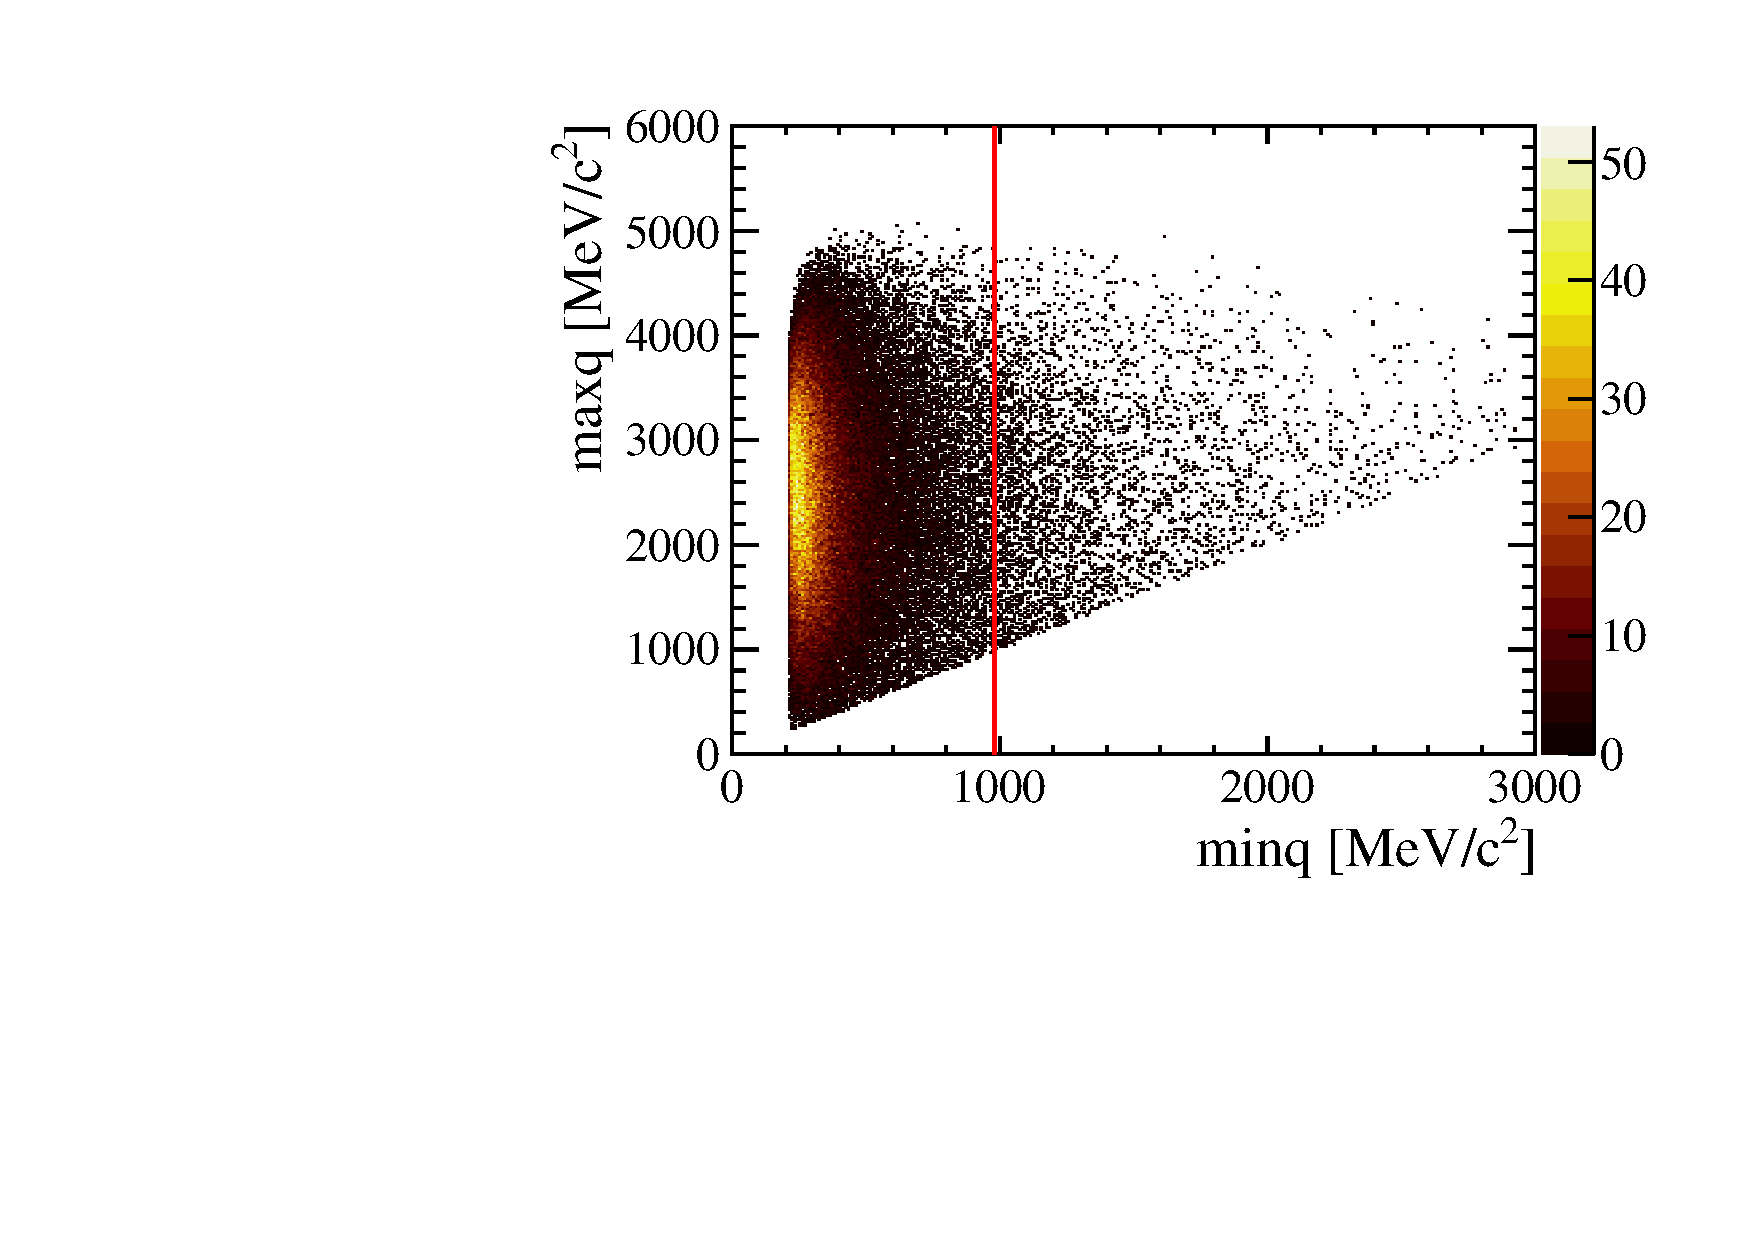
\includegraphics[width=0.5\linewidth]{./sel/scatterplotiatko_qmin.pdf}\put(-70,133){(a)}
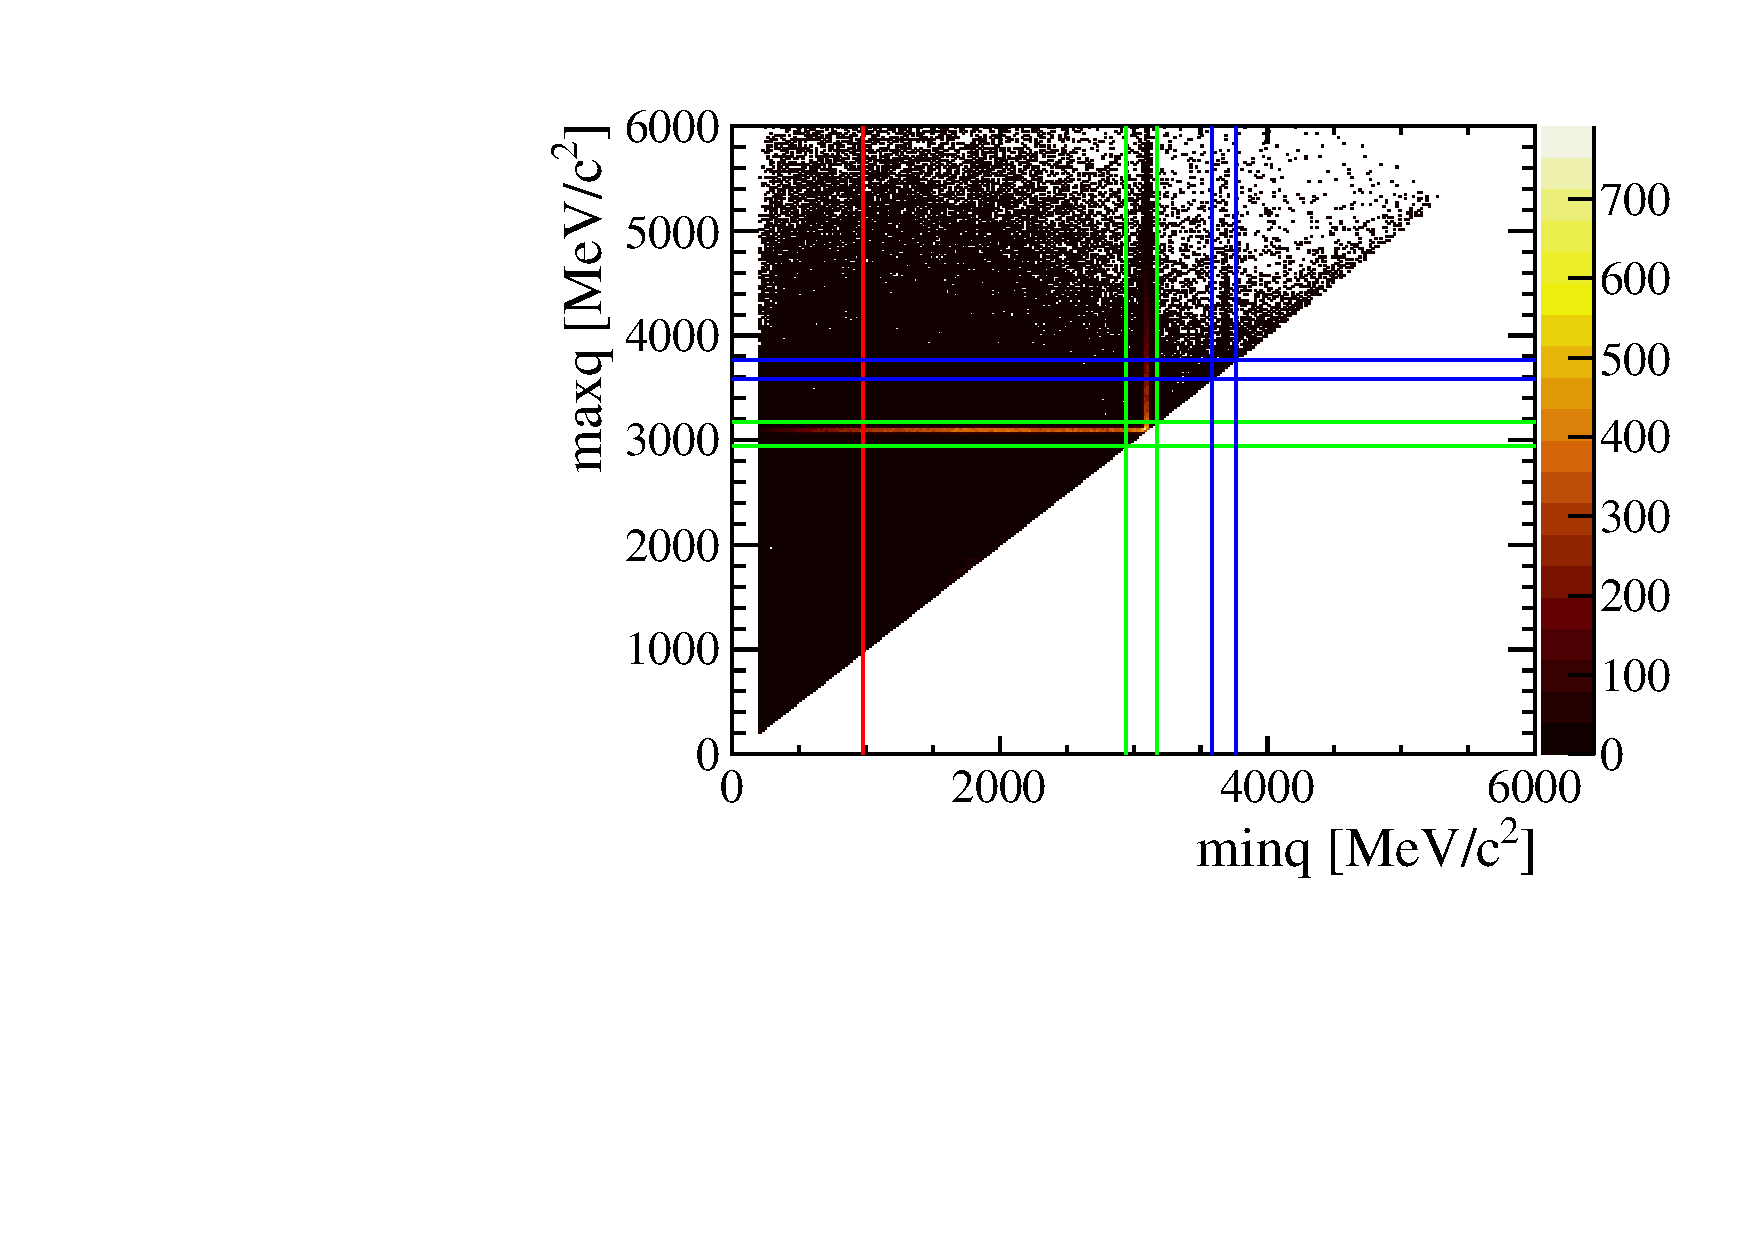
\includegraphics[width=0.5\linewidth]{./sel/scatterplotiatko_qmin_combidata.pdf}\put(-50,133){(b)}
\caption{(a) Signal simulation sample distribution in $minq$ and $maxq$ variables. Values below 980 \mevcc (red line) are accepted. (b) Combinatorial data sample after \textit{stripping} selection with no other cuts shows clearly the $J/\psi$ (green) and $\Psi(2S)$ (blue) resonances which are vetoed and the measurement region (red).}
        \label{fig:qsqsel}
%\vspace*{-1.0cm}
\end{figure}



\begin{table}[h!]
\begin{center}
\begin{tabular}{l c c}\toprule
	Veto & $q$ [\mevcc]  \\ \hline
        J/$\psi$  & !(2946.0 $<$ $q$ $<$ 3176.0)  \\
	$\Psi$(2S) &  !(3586.0 $<$ $q$  $<$ 3766.0)  \\
        \bottomrule
\end{tabular}
\end{center}
\caption{Vetoes for $J/\psi$ and $\Psi(2S)$ resonances. As $minq< 980 \mevcc$, these vetoes apply to $maxq$ combination only. }
\label{tab:vetoes}
\end{table}

\section{Further Selection}

Further selection is performed with the executive summary in~\autoref{tab:OfflineSelection}. This selection aims to further suppress backgrounds with different treatment in Run \Rn{1} and Run \Rn{2} due to the different definitions of variables, which was shown in~\autoref{bugs}. The sections below comment on the more exact features of this further selection. 

\begin{table}[h!]
%\small
\begin{center}
\begin{tabular}{l c c c}\toprule

%    \begin{tabular}{ | l | c |  } %p{7cm}|}
      Idea & Object & Run \Rn{1} Selection & Run \Rn{2} Selection \\ \hline
      Clean & Muon & - & \texttt{IsMuonTight==1.0}\\
      Clone and ghost & Muon & \texttt{Nshared==0} & \texttt{Nshared<2} \\
       & & in~\autoref{bugs} & \\
      Fit Region & $B$ & $4000 <M_{B_{corr}}<7000\mevcc$ & Same as Run \Rn{1} \\
       & &  in~\autoref{fittingsel} & \\
      Bkg Removal & event & Combinatorial BDT & Combinatorial BDT \\    
       &  & selection &  selection \\    
       &  & in~\autoref{CombiBDTsel} & \\
      Bkg Removal & event & Misid BDT & Misid BDT \\
	&  & selection &  selection   \\    
	& &  in~\autoref{misidbdt} & \\
	Optimize \texttt{FOM} & Muon & \texttt{Probnnmu}>0.35 & Same as Run \Rn{1} \\
        & & in~\autoref{furtherpid} & \\
%	\multicolumn{4}{c}{(\texttt{FOM}  defined ~\autoref{eq:punzifom})} \\
      \bottomrule
%      Clean & Min Dimuon & min $q^{2}(\mu^{+},\mu^{-})$ $<$ 960400 MeV$^{2}$/c$^{4}$  & min $q^{2}(\mu^{+},\mu^{-})$ $<$ 960400 MeV$^{2}$/c$^{4}$ \\ \hline
      \end{tabular}
\end{center}
	\caption{Offline selection performed after \textit{stripping}. Differences can be seen between Run \Rn{1} and Run \Rn{2} datasets. \texttt{FOM} is defined int~\autoref{eq:punzifom}.}
\label{tab:OfflineSelection}
\end{table}

%The sections below comment on the more exact features of this further selection. 

	\subsection{General Features of Multivariate Selections}

All the multivariate classifiers in the search for the \Bmumumu decay use TMVA's \cite{Speckmayer:2010zz} implementation of Boosted Decision Tree (BDT) with the \texttt{AdaBoost} algorithm. The multivariate selections used in the search for the \Bmumumu decay are the isolation BDT detailed in~\autoref{isolationvar}, the combinatorial BDT detailed in~\autoref{CombiBDTsel} and the misid BDT detailed in~\autoref{misidbdt}.

The background characterisation study of inclusive $b\bar{b}$ simulation shows that there are two dominating backgrounds, combinatorial background and misID background. In order to reduce these backgrounds, two consecutive multivariate classifiers are used. The first multivariate classifier is developed to remove efficiently combinatorial background and a second multivariate classifier will help to control the contamination from misID decays. One of the key variables that provide the greatest separation power in these two multivariate classifiers is another BDT output, the isolation BDT.

Cross-validation is one of the useful methods used within MVAs which improves the chance of good performance of the predictive model on an independent dataset. In this way, biases due to naive sample split into training and testing subsample, could be overcome. In general, it helps also with overfitting when the model of the classifier is sensitive to fluctuations.  The cross-validation method used in both combinatorial BDT and misid BDT is known as the \textit{k-folding} technique \cite{kfold}. 

In particular, both background and signal samples are randomly split into $k$ similar size subsamples. Then the BDT is trained on the $k-1$ signal/background subsamples, which are subsequently tested on the remaining last subsamples. This process is repeated $k$-times for all possible combinations, hence the name of cross-validation. In the last step, the results for all the sample are produced by amalgamating the values obtained from the tested $k$ subsamples. In the combinatorial and misid BDT, there are 10 folds used. Both of the BDT classifiers use the same set of variables listed in~\autoref{tab:vars}.

\begin{table}[h!]
\begin{center}
\begin{tabular}{| l  l  l |} \hline
$B^{+} p$ & \gls{minipchi2} of all three muons & \gls{DIRA} \\
$B^{+}$ $p_T$ & $p_{T}$ of all three muons & $B^{+}$ \gls{fdchi2} \\ 
$B^{+}$ \gls{vertexchi2ndof} & \gls{minipchi2} of all three muons  & Isolation variable \\
	$B^{+}$ lifetime &  & (~\autoref{isolationvar}) \\ \hline
\end{tabular}
\end{center}
\caption{BDT variables used in both combinatorial and misID Run \Rn{1} and Run \Rn{2} BDTs.}
\label{tab:vars}
\end{table}



	\subsection{The Isolation Boosted Decision Tree}
\label{isolationvar}

\begin{figure}[h!]
\centering
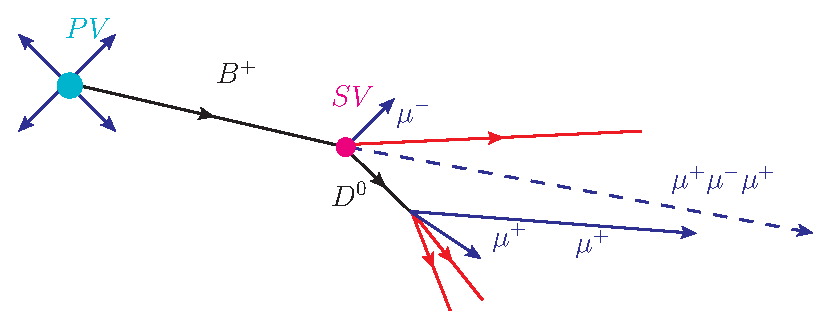
\includegraphics[width=0.45\linewidth]{./sel/Isolation.eps}\put(-70,60){(a)}%
\hspace*{1.0cm}
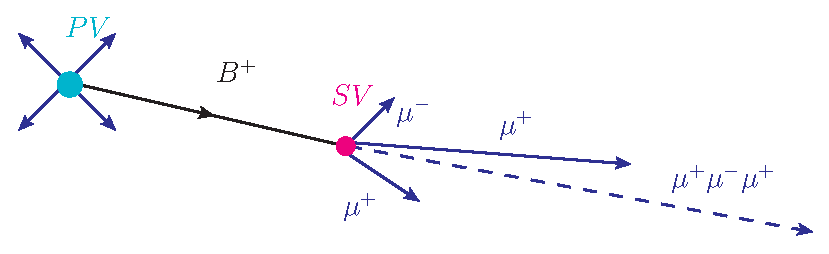
\includegraphics[width=0.45\linewidth]{./sel/Isolation_Signal.eps}\put(-70,60){(b)}
	\caption{An example of decay topology for (a) background and (b) signal.}
\label{fig:isolation1}
%\vspace*{-1.0cm}
\end{figure}	
\noindent The vast majority of the backgrounds that share the possibility of contaminating \Bmumumu signal have one property in common: they have more tracks associated with the decay. It is hence possible to use multivariate analysis (MVA) techniques to establish how \textit{isolated} the signal trimuon vertex is as compared to a background trimuon vertex as seen in~\autoref{fig:isolation1}.
	
%	In an event, for both signal and misidentified background there is a possibility that neutral particles, charged tracks or even a combination of both cases had not been reconstructed in the given vertex.

The isolation quality of the vertex is determined with a BDT. This regression algorithm classifies the event to be more signal-like or background-like according to different track and vertex properties, the \textit{isolation variables}. The \textit{isolation variables} include track $p_T$, the opening angle between track's momentum and momentum of the combined signal/background visible system, the \gls{trackchi2ndof}, the ghost probability of the track \gls{pgh2}, \gls{ipchi2} of the track with respect to signal/background \gls{SV} and \gls{PV}.


The signal proxy for the isolation BDT was trained and tested with a $\Lambda^{0}_{b}\rightarrow p \mu^{-} \bar{\nu}$ simulation sample, where all tracks apart from the $p \mu^{-}$ signal tracks are taken into account.
%no tracks vertex well
The background sample consists of trakcs of $\Lambda_{c}$ vertex from  $\Lambda^{0}_{b} \rightarrow (\Lambda_{c} \rightarrow p X) \mu^{-} \bar{\nu}$ decays, disregarding the $p \mu^{-}$ tracks (i.e the $X$). The isolation BDT is based on the weights obtained from these samples, which are computed in \cite{Aaij:2015bfa}. These weights are applied to the \Bmumumu signal and background proxies, as they share similar topology with respect to isolation properties. In other words, track density is different between signal and background. 


The Isolation BDT response peaks between -1 and 0 for isolated tracks (signal-like) and between 0 and 1 for non-isolated tracks (background-like). An event is considered signal-like if all other tracks apart from $p \mu^{-}$ tracks in the event are isolated from the $p \mu^{-}$ vertex. The output of this BDT for both types is shown in~\autoref{fig:isolation}. Backgrounds shown include combinatorial background and misID type background. In the analysis, there is no explicit selection on this variable, but it is used as one of the input variables for the combinatorial and misid BDTs.

\begin{figure}[ht]
\centering
	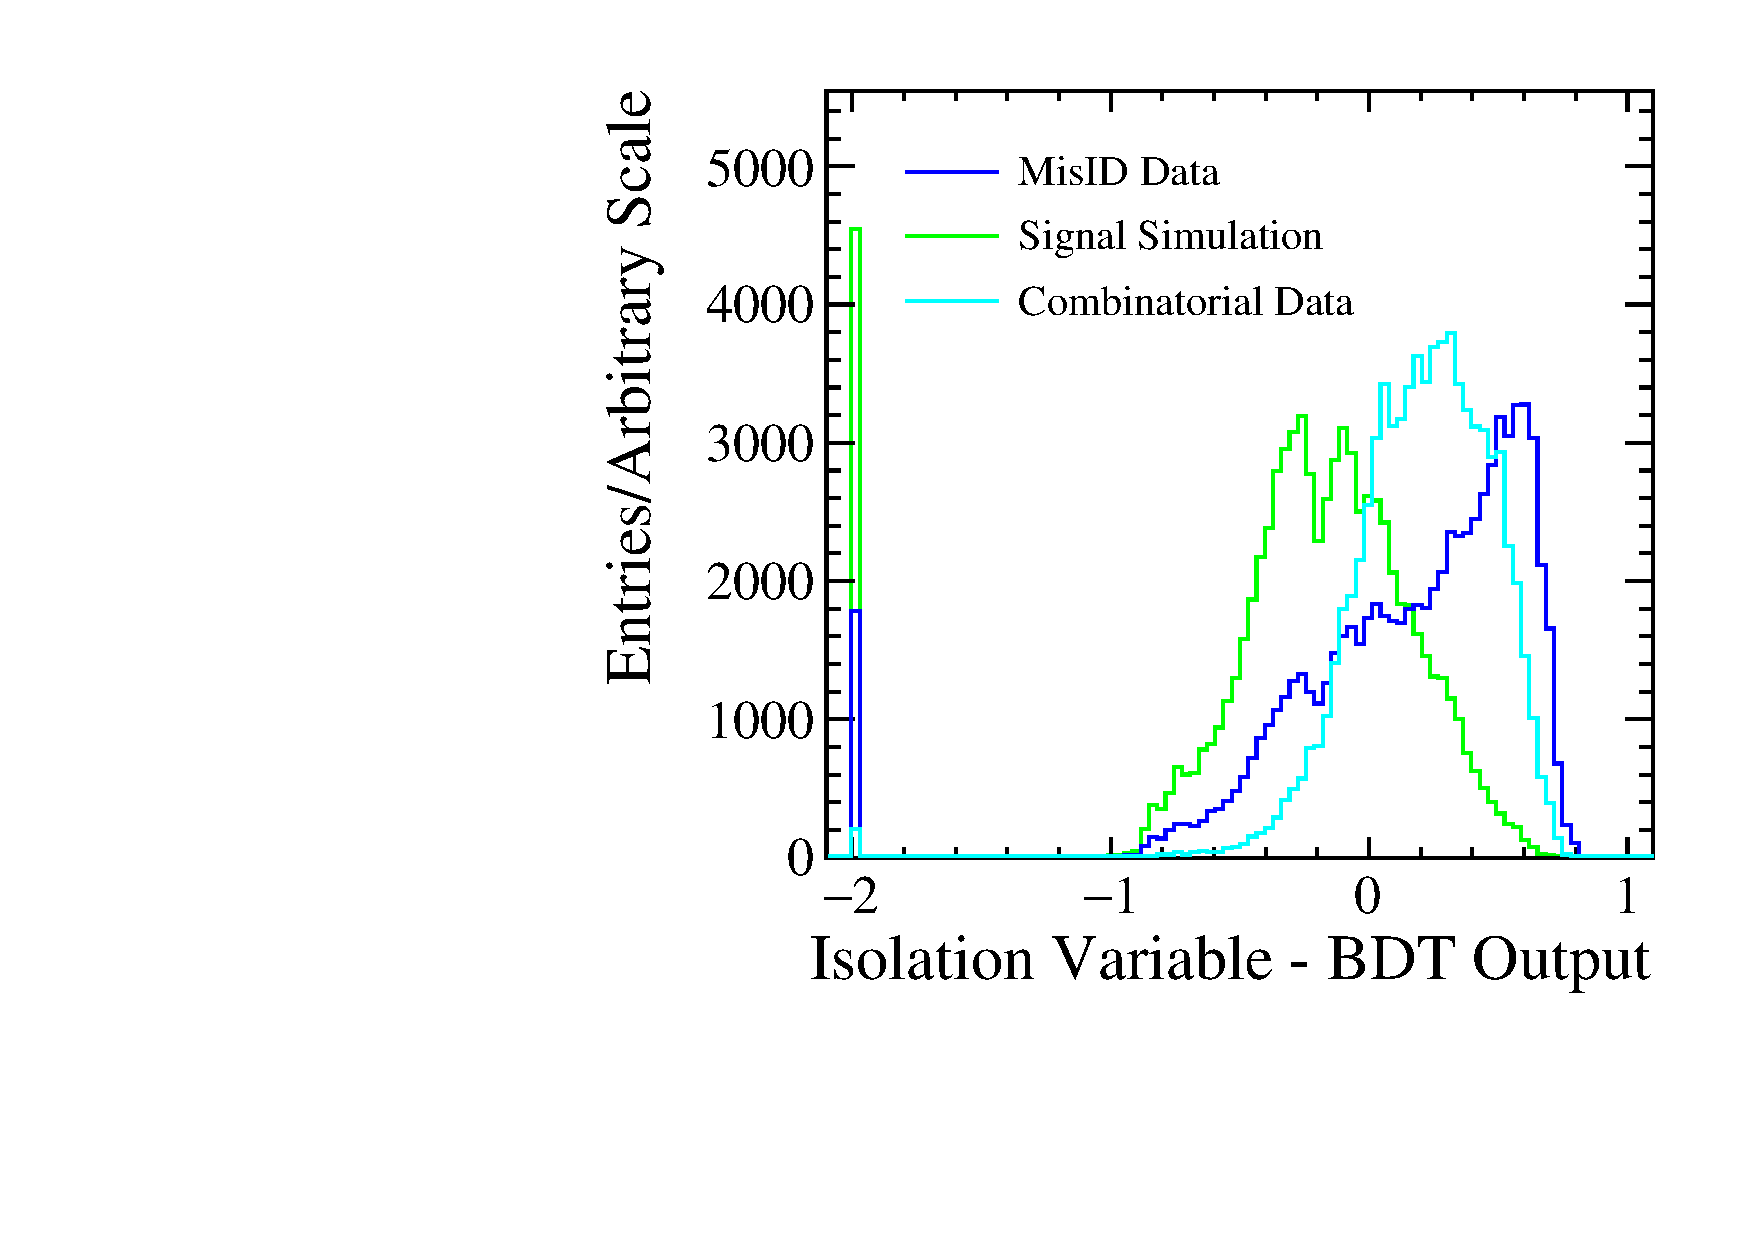
\includegraphics[width=0.5\linewidth]{./sel/Thesis_variableBplus_pmu_ISOLATION_BDT1_weightsbeforeq22012.pdf}{\put(-50,133){(a)}}%
	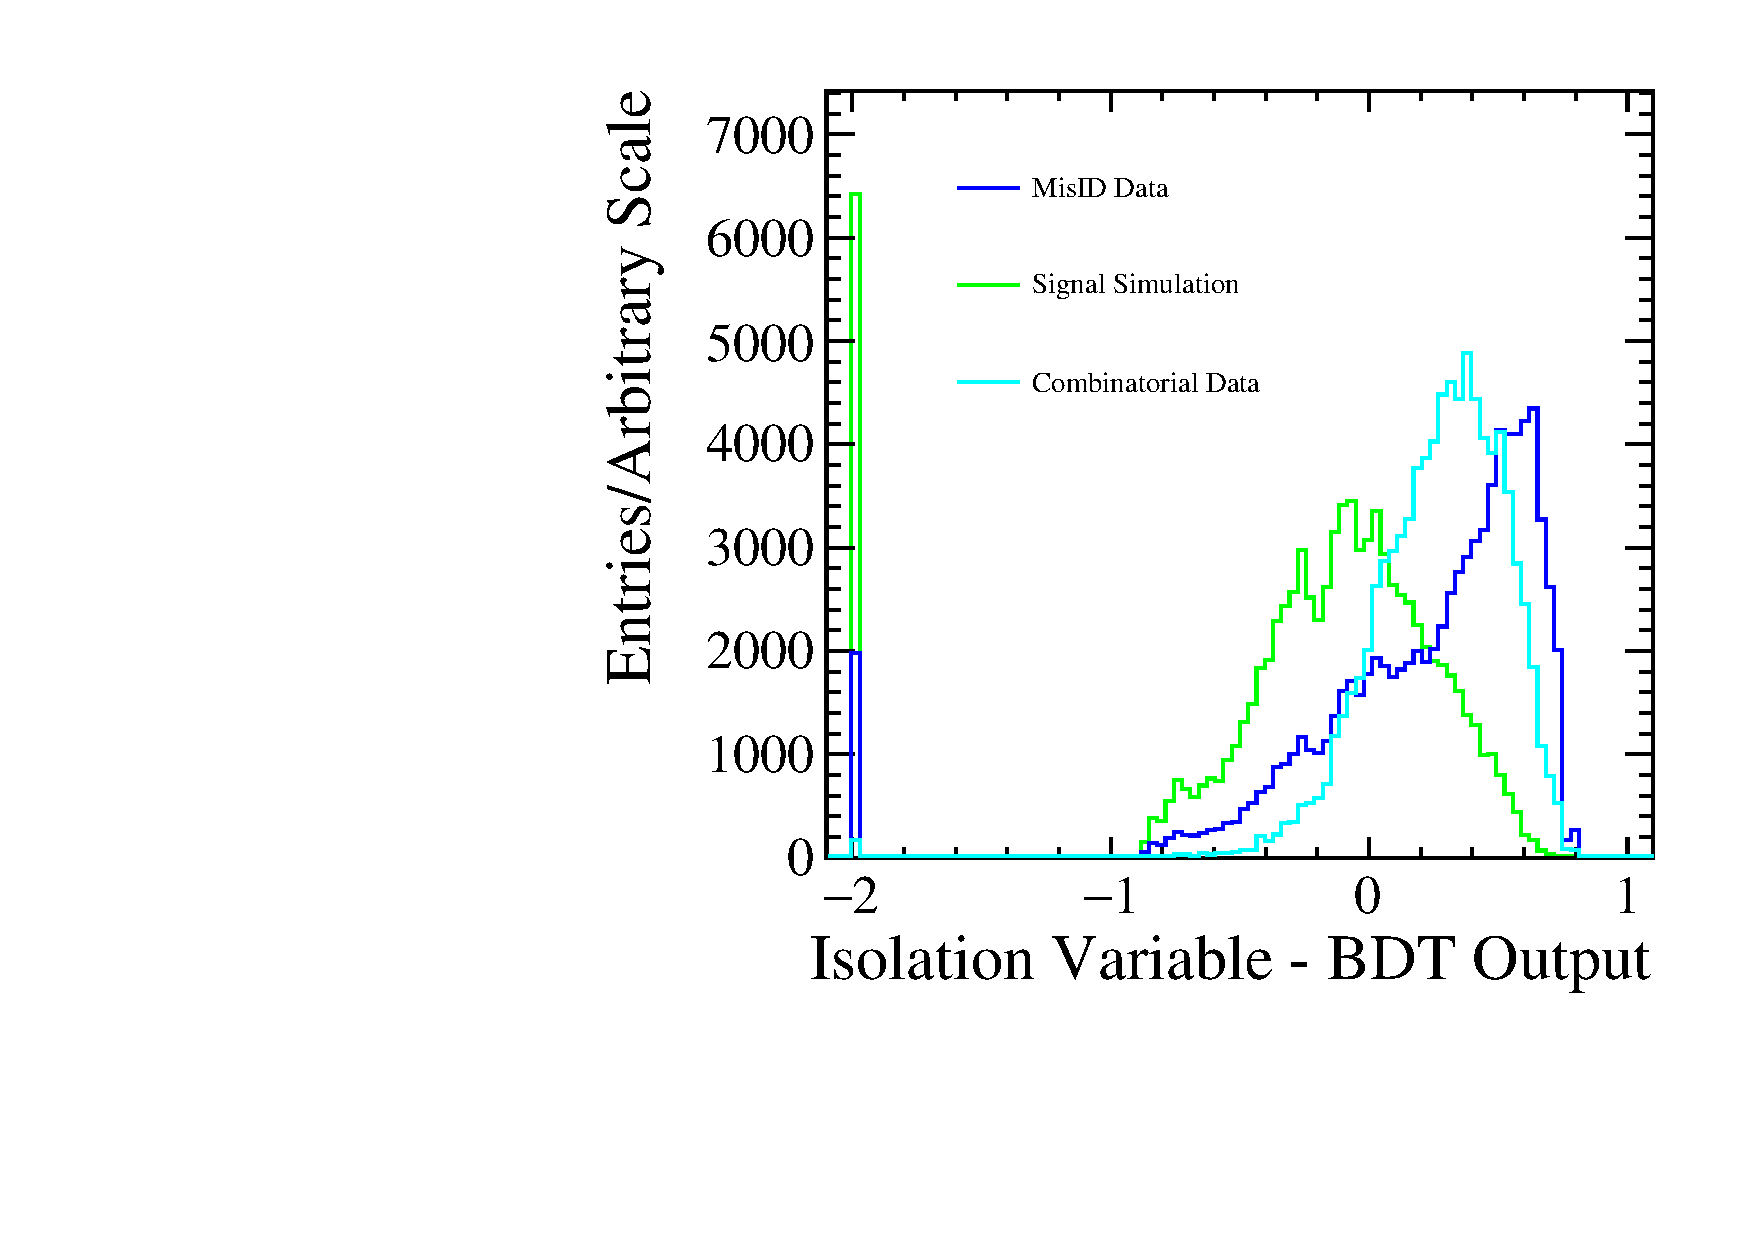
\includegraphics[width=0.5\linewidth]{./sel/Thesis_variableBplus_pmu_ISOLATION_BDT1_weightsbeforeq22016.pdf}{\put(-50,133){(b)}}
	\caption{Isolation score for signal and backgrounds using (a) Run \Rn{1} (b) Run \Rn{2} samples. If isolation fails to find any other track than $p \mu^{-}$ tranks in the event, by default it gives value -2.}
\label{fig:isolation}
\end{figure}

\subsection{The Combinatorial Boosted Decision Tree}
\label{CombiBDTsel}
One of the most prominent backgrounds is combinatorial background and to reduce its contamination while keeping the signal efficiency as high as possible, a combinatorial BDT is trained.
To obtain the combinatorial BDT discriminant, a simulated sample for signal and the upper mass sideband data sample ($M_{B_{corr}}>5.5$ \gevcc) for background are used. These samples passed through the preselection, trigger, $q^{2}$ selection stages and are using the input variables mentioned in~\autoref{tab:vars}.

As the branching fraction and hence the number of signal events is unknown, the metric known as the Punzi figure of merit \texttt{(FOM)} \cite{Punzi:2003bu}, is used to find an optimal working point. It is defined as

\begin{equation}
	\texttt{FOM}=\frac{\varepsilon_{S}}{\sqrt{B}+\sigma/2},
	\label{eq:punzifom}
\end{equation}
where $\varepsilon_{S}$ is the signal efficiency of the selection, $B$ refers to the number of background candidates and $\sigma$ is the significance that the analysis aims to minimally achieve. %In this case, the significance of 3$\sigma$ is used. The advantage of this \texttt{FOM} to more conventional one is that is it insensitive to the knowledge of exact number of signal events, which is the case as the branching fraction is unknown.
In this case, the significance 3$\sigma$ is used, but it was checked that there is no change to the optimal working point if it is varied to $5\sigma$, as seen in~\autoref{fig:punzifom}.

\begin{figure}[ht]
\centering
	\includegraphics[width=0.5\linewidth]{./sel/Scaled_nice_FOM_Run1.pdf}%
	\includegraphics[width=0.5\linewidth]{./sel/Scaled_nice_FOM_2016.pdf}%
	\caption{ Punzi \texttt{FOM} shows the optimum working point at 0.47 for Run \Rn{1} and 0.54 for Run \Rn{2} as seen in both figures with a violet line for $\sigma=3$ and $\sigma=5$. This \texttt{FOM} is for Combinatorial BDTs.}
\label{fig:punzifom}
\end{figure}


The \texttt{FOM} is computed in the blinded mass region, $4.5\gevcc <M_{B_{corr}} <5.5$ \gevcc. To estimate the number of background candidates in the blinded region, the final fit strategy described in~\autoref{fitsens} is used to fit the data, yielding around $10000$ in Run \Rn{1}, and $9000$ combinatorial candidates in Run \Rn{2}. The yields are extracted from blinded fits to data by integrating the combinatorial part of the total background probability density function (PDF) in the blinded region.

In order to accommodate different selections between Run \Rn{1} and Run \Rn{2}, separate BDTs are trained for different Runs. Combined training of all of the datasets was also performed but it does not lead to any improvement in background rejection. Results of the comparison between separate and combined training can be seen in ~\autoref{fig:separatetraining}. Different intrinsic properties (such as the number of trees used) and variables (such as two-particle vertices) have been explored but no improvement in discrimination of the BDT was achieved.


\begin{figure}[ht]
\centering
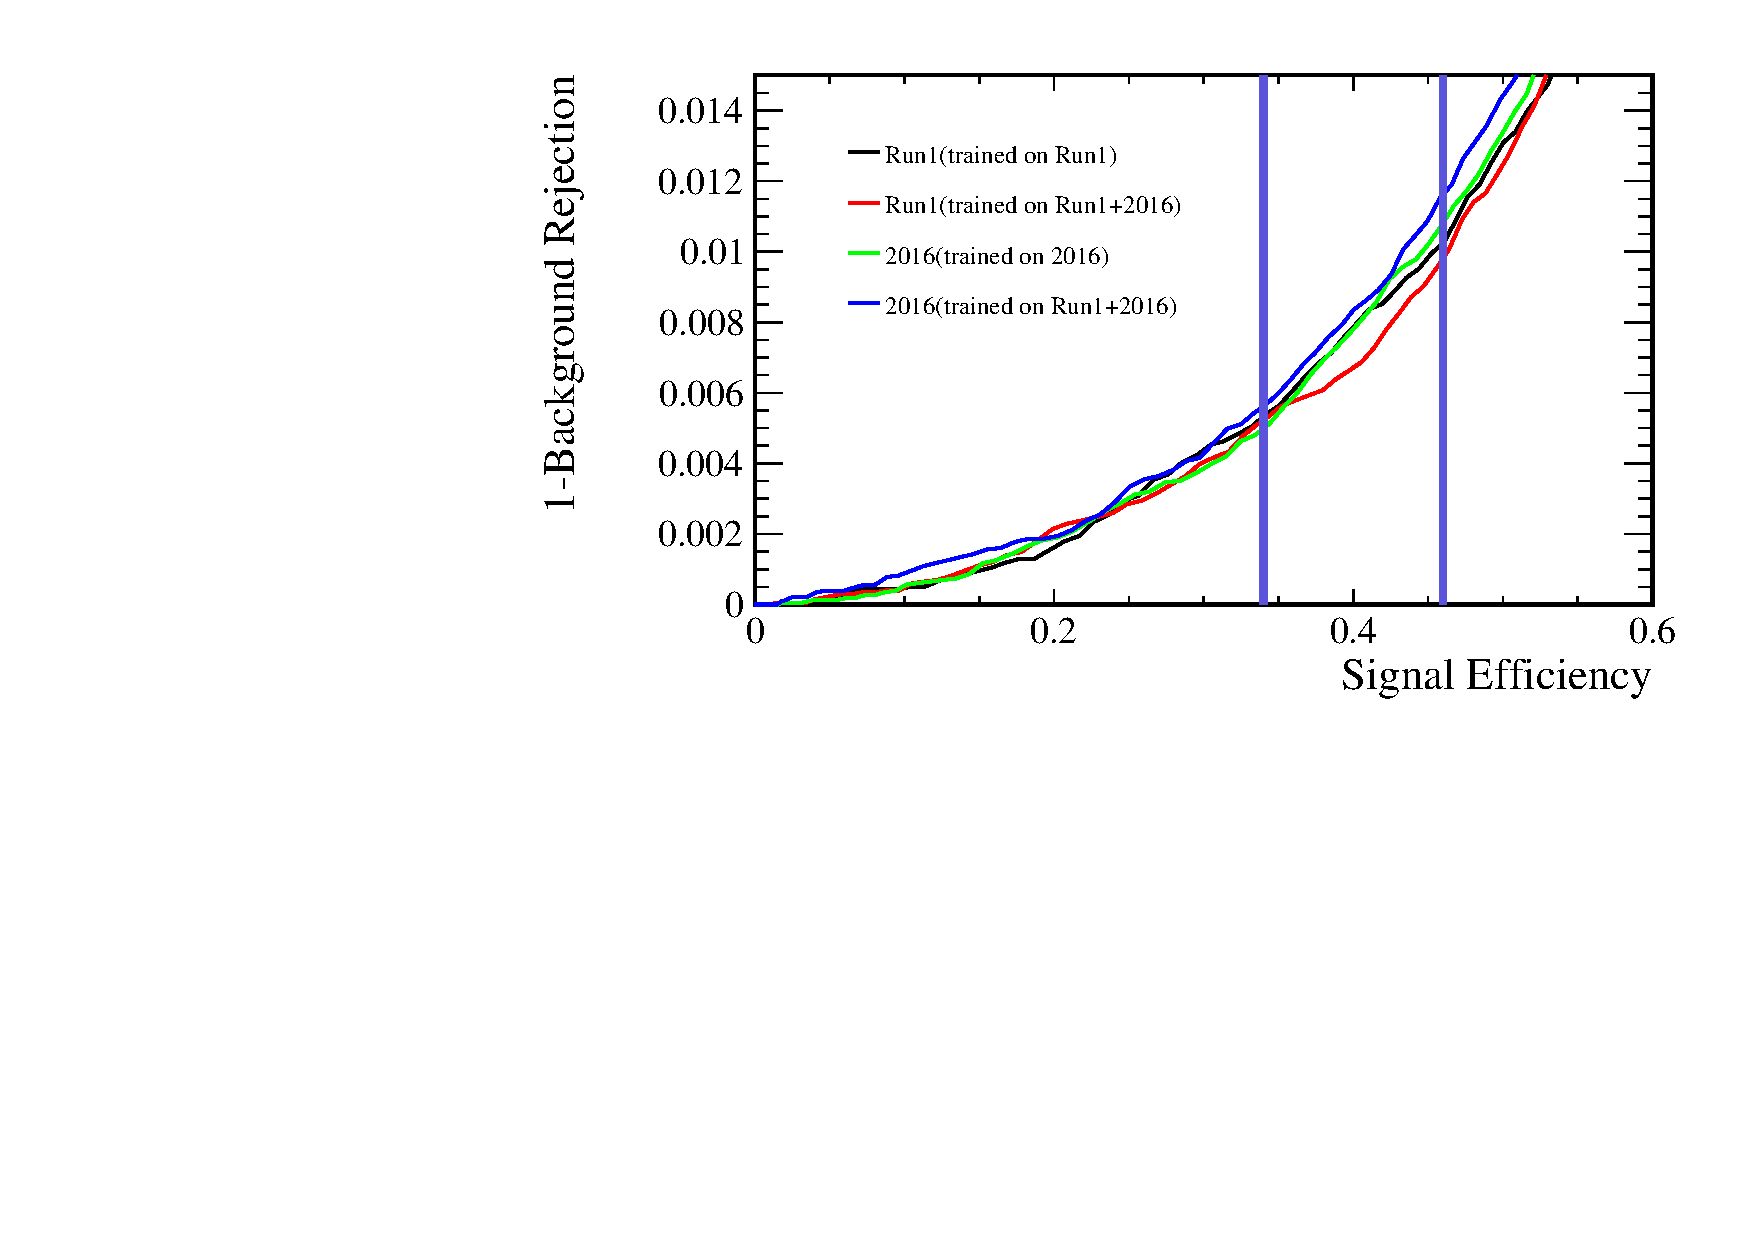
\includegraphics[width=0.8\linewidth]{./sel/final_comparison_from_root_combi_2.pdf}
	\caption{Comparison of separate and combined training samples and performance on different datasets. Two vertical violet lines represent optimal points in the signal efficiency, for Run \Rn{1} (0.47) and for 2016 (0.34) where the working point of the two BDTs are chosen. Separate training provides greater rejection power in 2016. In Run \Rn{1} training on both datasets provides comparable performance for given optimal signal efficiency. Taking into the account the fact that selection slightly differs for 2016, it is advantageous to keep the BDTs separate.}
%\vspace*{-1.0cm}
\label{fig:separatetraining}
\end{figure}




In both Combinatorial BDTs, the most discriminating variables are the isolation variable (described in~\autoref{isolationvar}), $B^{+}$ \gls{vertexchi2ndof}, \gls{minipchi2} of the muons and $p_{T}$ of the $B^{+}$ meson. Combinatorial muon comes more from somewhere else in the event and hence its \gls{minipchi2} is worse as compared to the signal, making $B^{+}$ \gls{vertexchi2ndof} worse. Moreover, as this combinatorial muon comes from somewhere else, other tracks may accompany it making the isolation variable a good discriminant. The combinatorial muon also tends to have higher momentum and hence $p_{T}$ of the $B^{+}$ is higher. Distributions for these different variables can be seen in~\autoref{fig:discombi}. 


\begin{figure}[ht]
\centering
	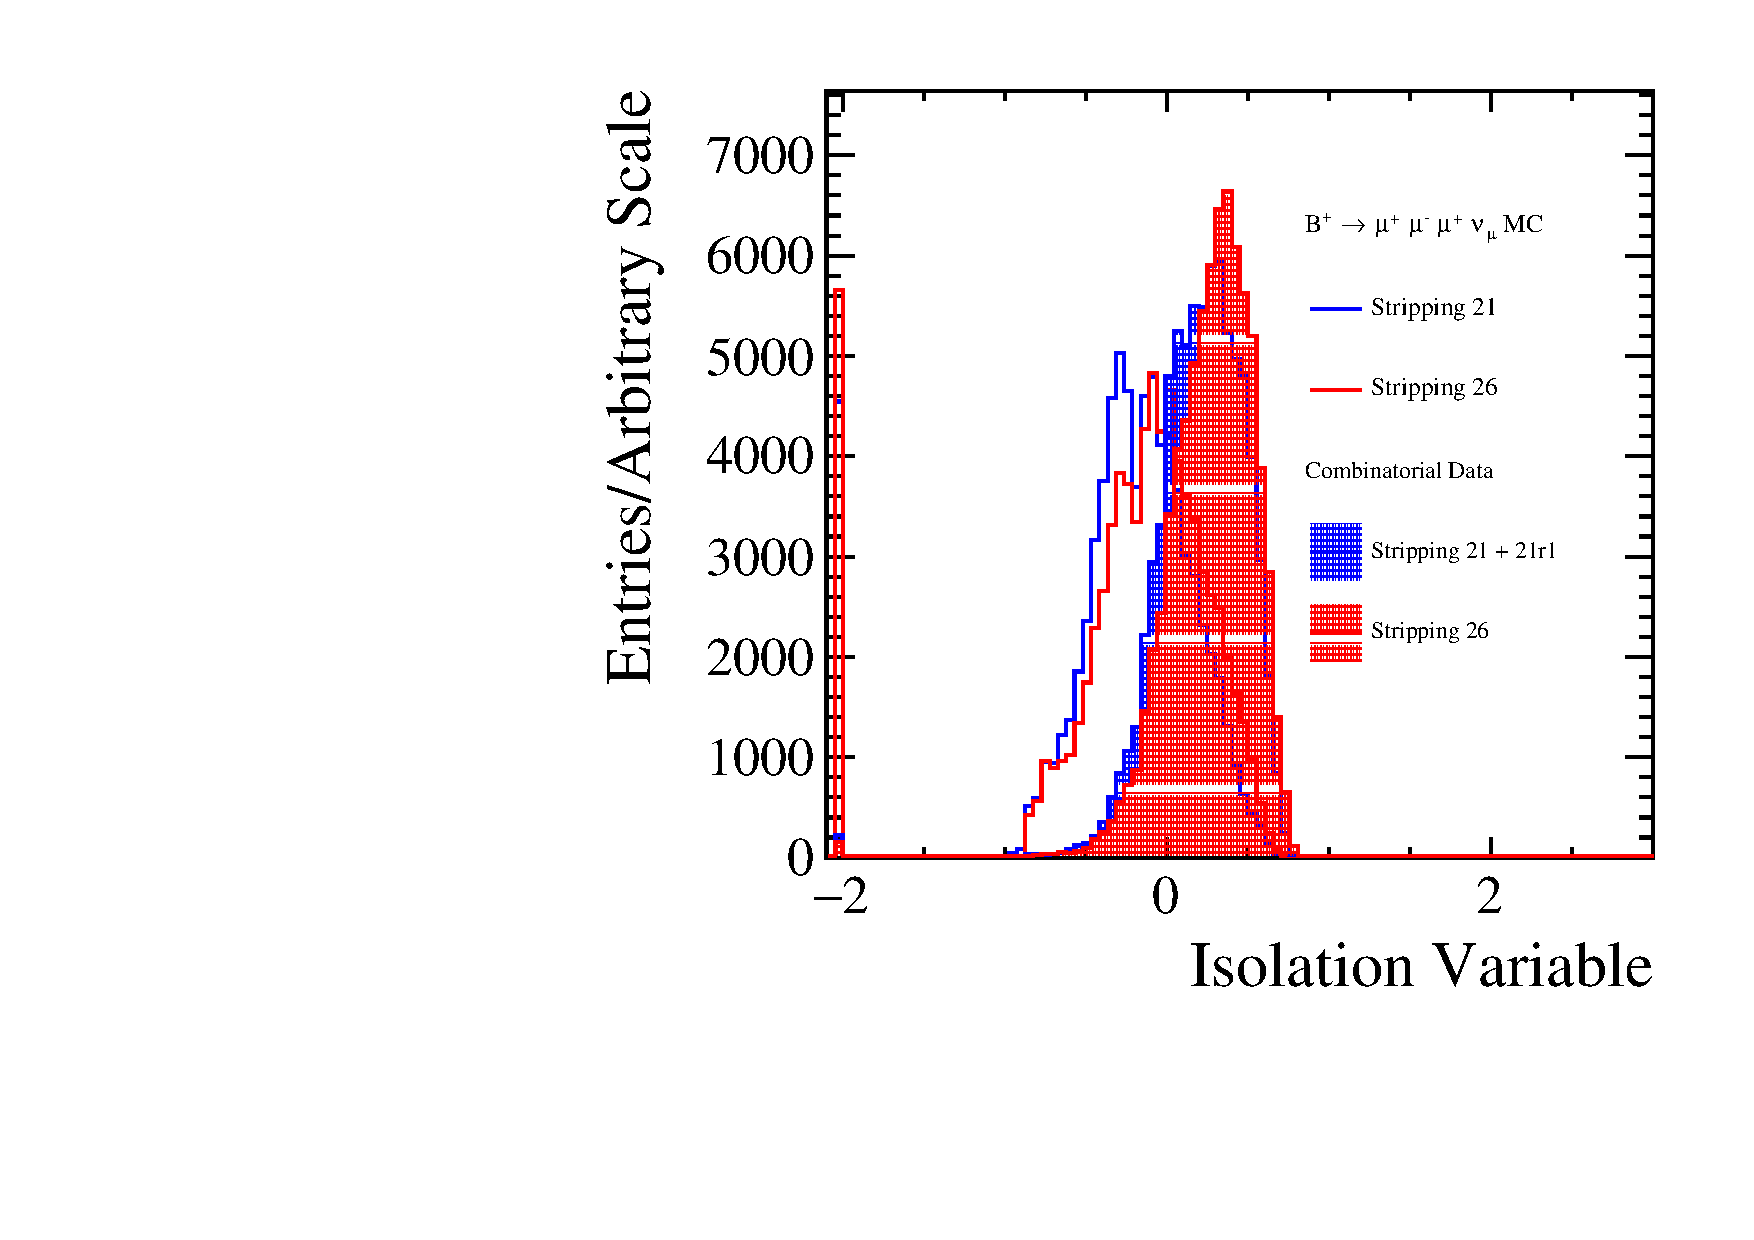
\includegraphics[width=0.5\linewidth]{./sel/combi/plotvariableBplus_pmu_ISOLATION_BDT1_weightsNICEDISMIX.pdf}%
	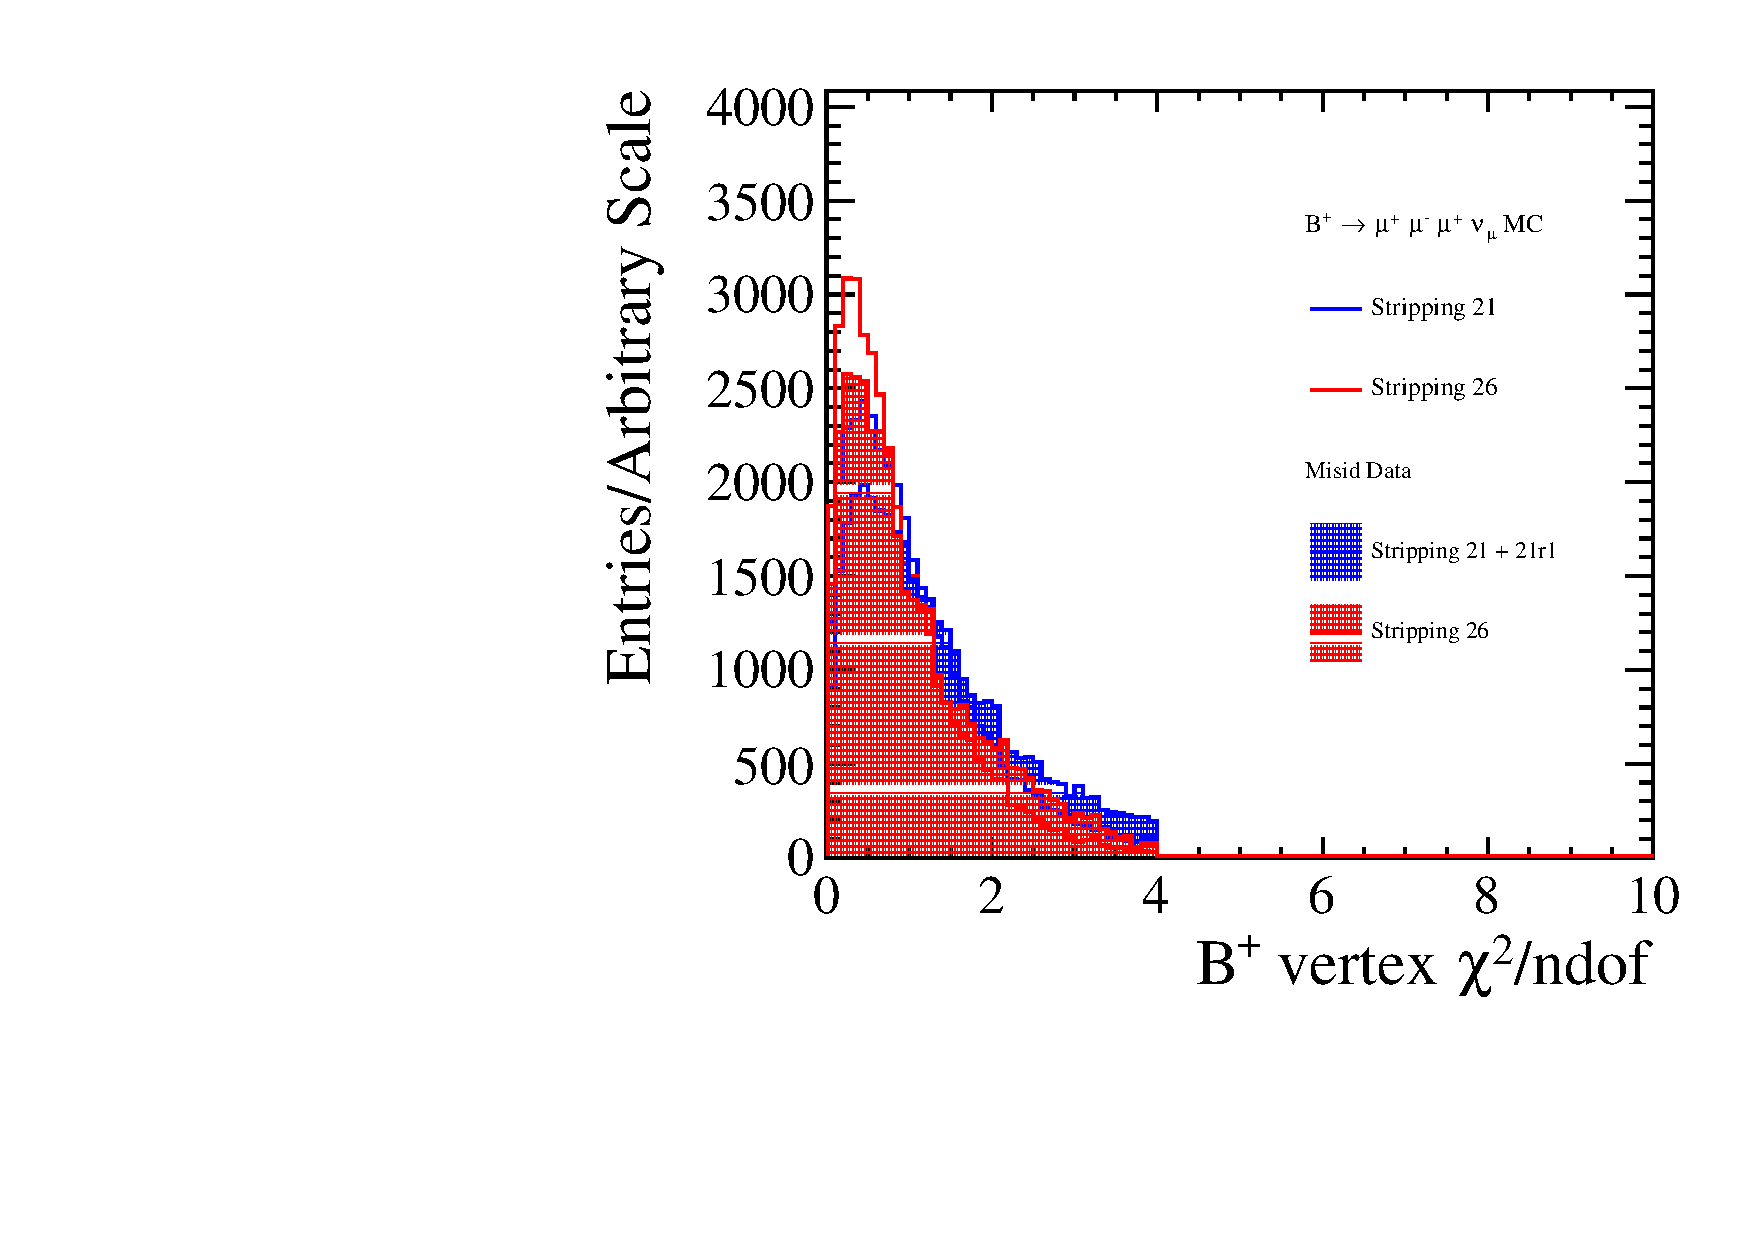
\includegraphics[width=0.5\linewidth]{./sel/combi/plotvariableBplus_ENDVERTEX_CHI2NICEDISMIX.pdf}%
	\newline
	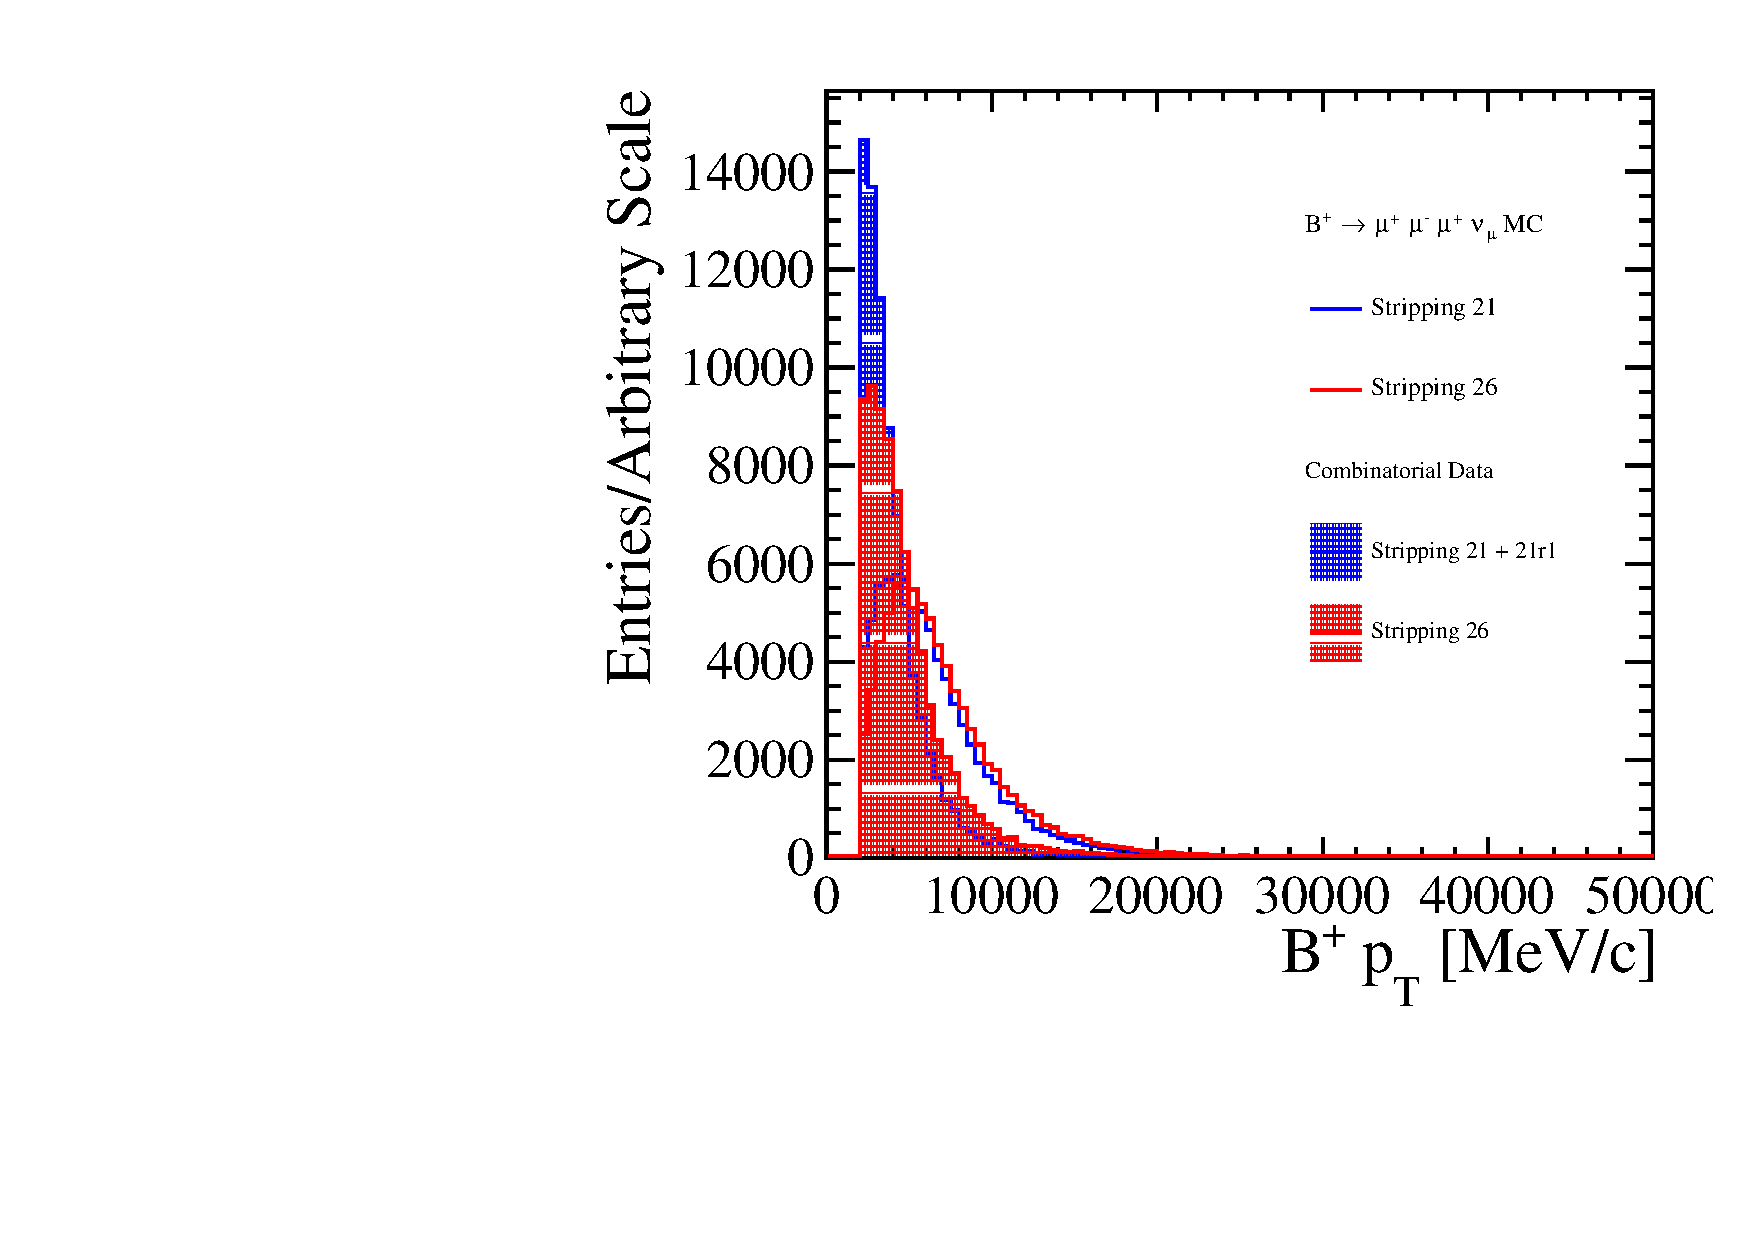
\includegraphics[width=0.5\linewidth]{./sel/combi/plotvariableB_PTNICEDISMIX.pdf}%
	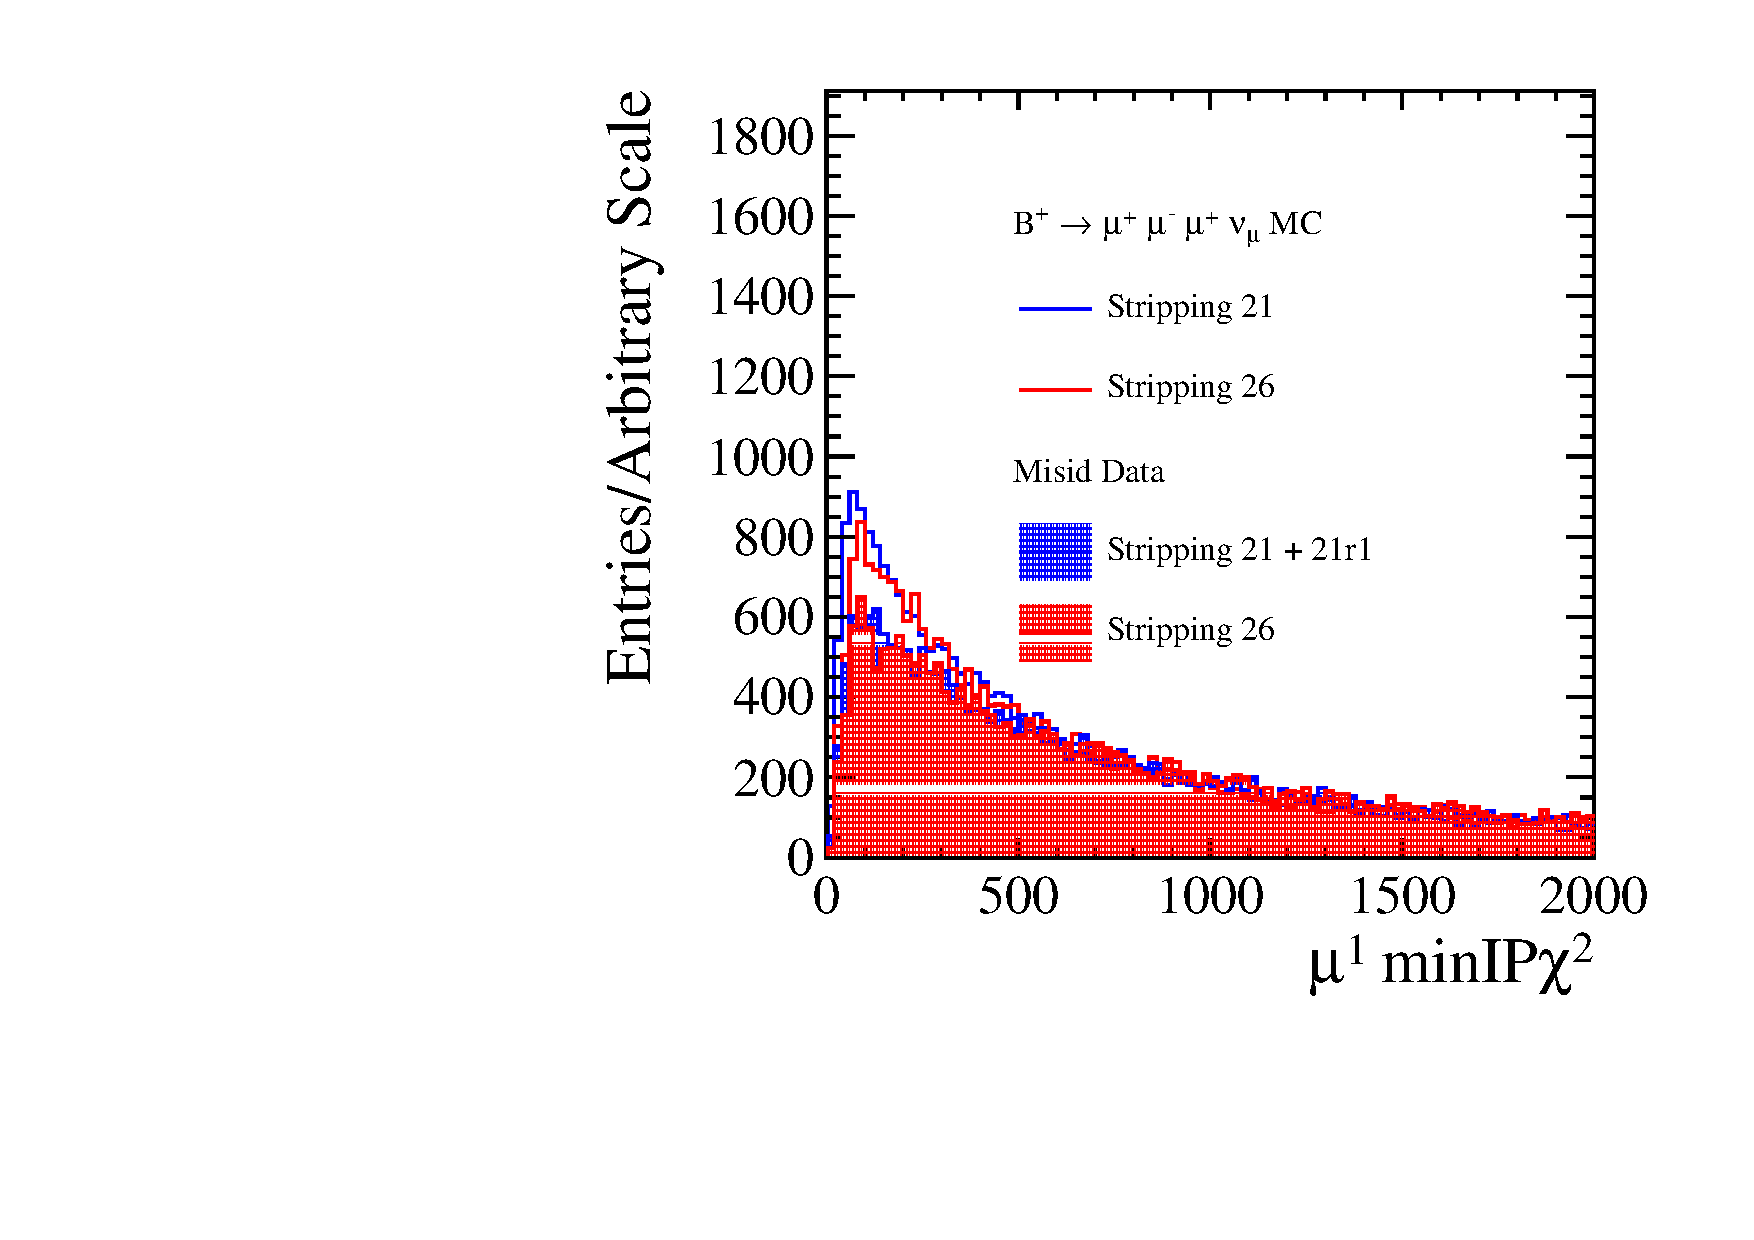
\includegraphics[width=0.5\linewidth]{./sel/combi/plotvariablemu1_MINIPCHI2NICEDISMIX.pdf}%
	\caption{The variables with the most discriminative power for both Run \Rn{1} and 2016 Combinatorial BDTs.}
\label{fig:discombi}
\end{figure}


It is also important that there is no skewing of the mass distribution for the background as this could lead later to modelling issues with these different background components. This was checked by looking at the behaviour of BDT output in different bins of $M_{B_{corr}}$. If the BDT value stays flat then the background will not be skewed, which is the case for Run \Rn{2} as seen in~\autoref{fig:flatnessofcombibdt}. This is also the case for Run \Rn{1}. 


\begin{figure}[ht]
\centering
	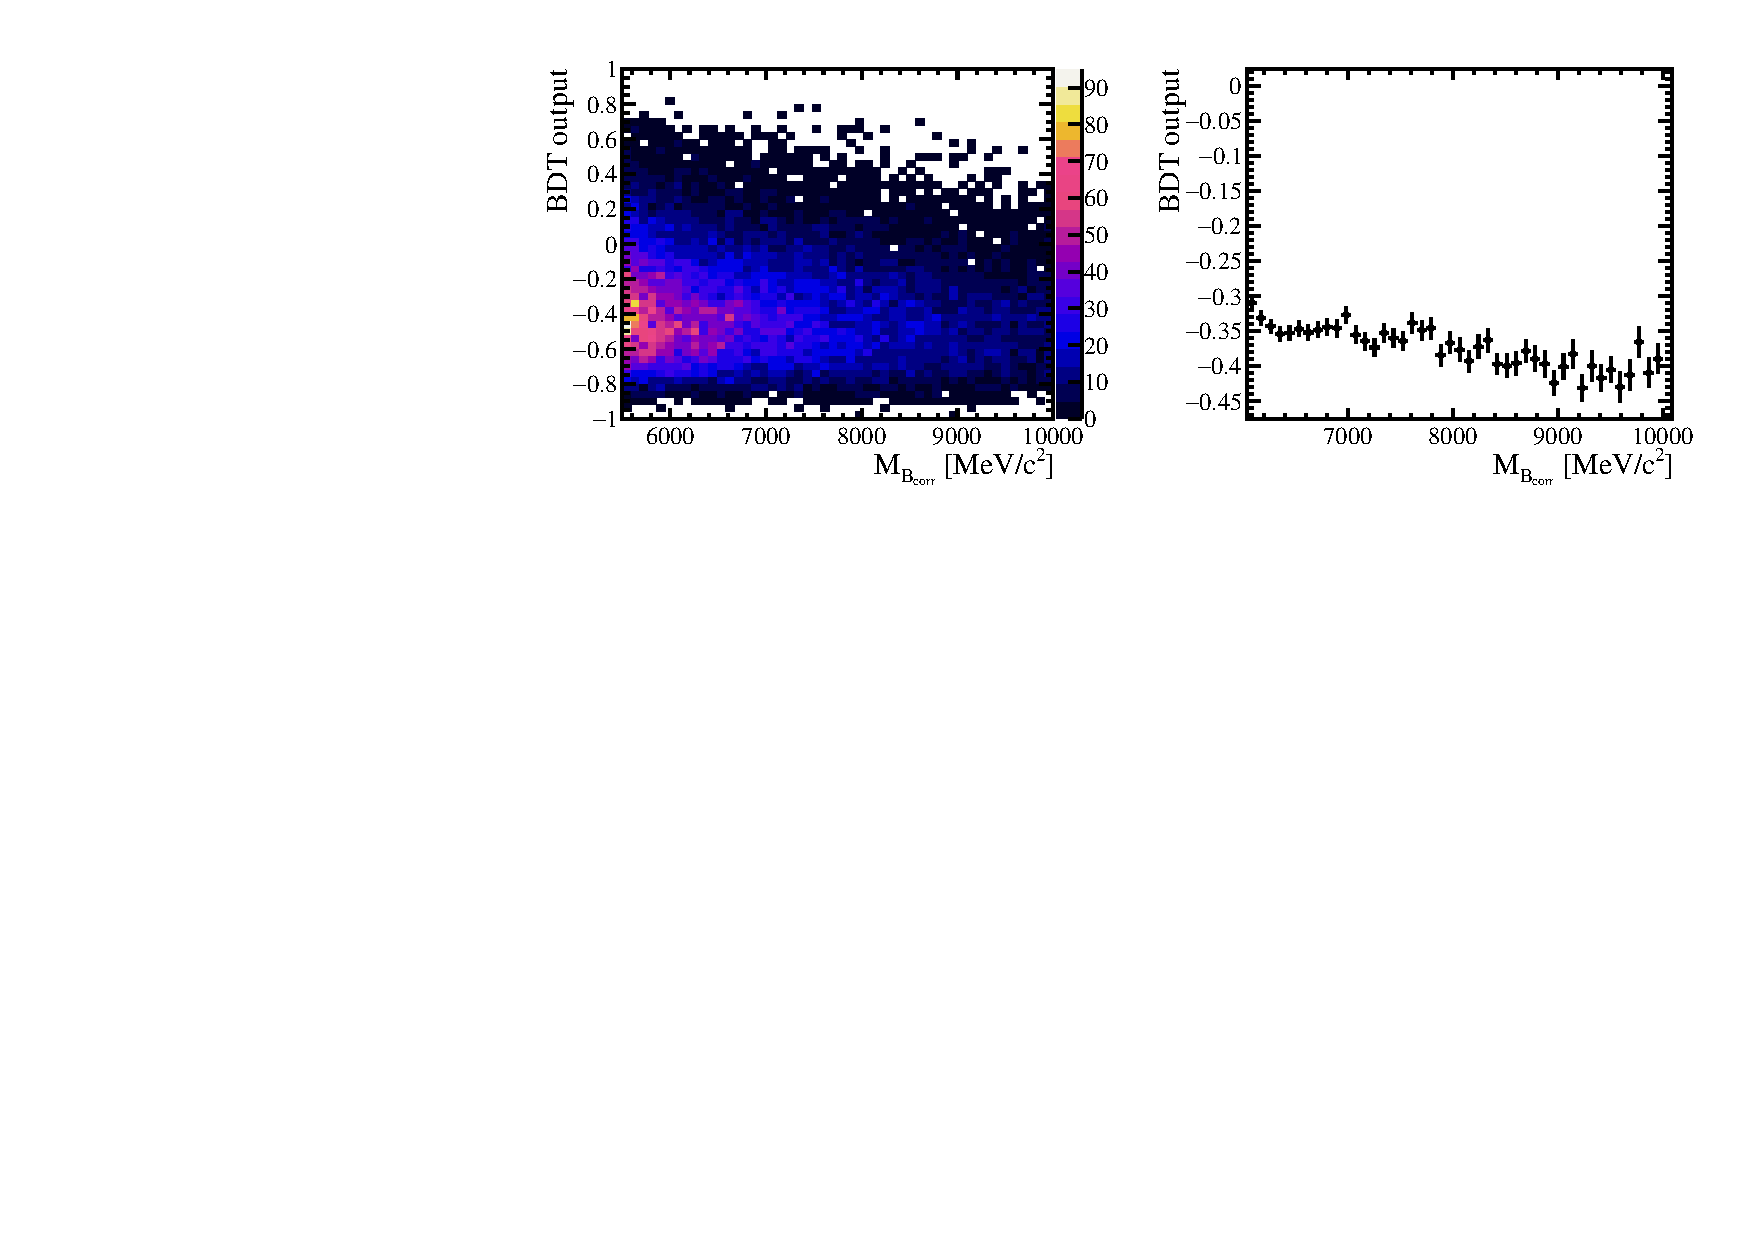
\includegraphics[width=1.0\linewidth]{./sel/CombiBDT_ProfileX_of_Bplus_Corrected_Mass_vs_MCSig2016_288888335_vs_DATACombi2016NTrees60_MinNodeSize2_MaxDepth3_SeparationTypeGiniIndex_PruneMethodNoPruning_DoPreselection_nice.pdf}
	\caption{Study of linear correlation between BDT output and $M_{B_{corr}}$ and BDT value for each bin of $M_{B_{corr}}$ in 2016 shows that the Combinatorial BDT is relatively flat as a function $M_{B_{corr}}$. The right plot shows the mean and uncertainty on the mean of the 2016 Combinatorial BDT in bins of the $M_{B_{corr}}$.\mybox{Sally: Error do rms instead of the standard error}.}
\label{fig:flatnessofcombibdt}
\end{figure}

\subsection{The Misid Boosted Decision Tree}
\label{misidbdt}
In the same way, the classifier that distinguishes well between signal and misID background was developed. The misID sample, that is used for training and testing, was obtained the same way as the signal but with one of the muons not identified as the muon. Rather, this third particle will be identified either as a proton, pion or kaon. More about the parametrisation of this background can be found in~\autoref{misidprocedure}. These samples went through all the previous selection including application of Combinatorial BDTs. As before, Run \Rn{1} and Run \Rn{2} are trained and used separately on the relevant datasets, as shown in~\autoref{fig:separatetrainingmis}. 


\begin{figure}[ht]
\centering
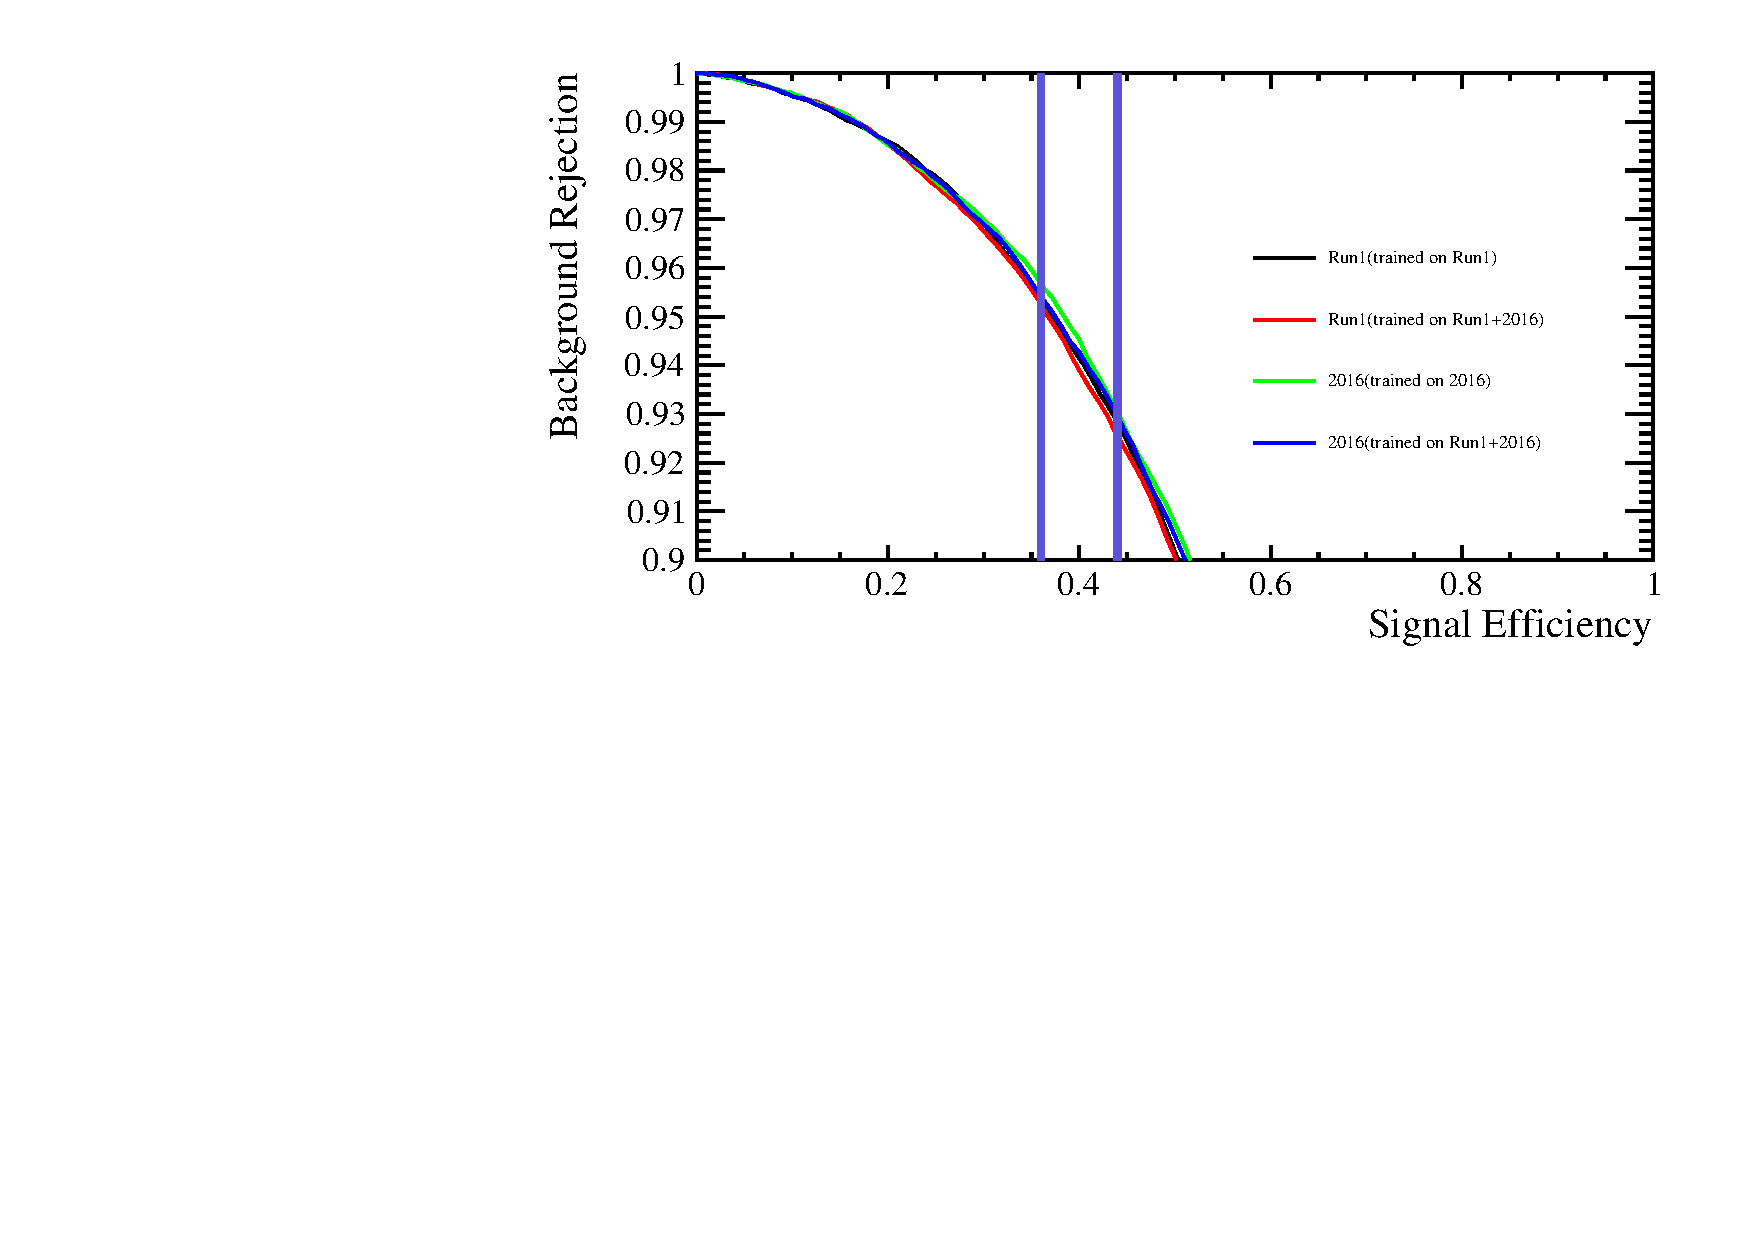
\includegraphics[width=0.9\linewidth]{./sel/true_Misid_CompareTrainOnBothRun1and2016__COMPAREroccurvesDIFFERENTtrainings.pdf}
	\caption{Comparison of separate and combined training samples and performance on different datasets. Optimal working point is chosen, see~\autoref{fig:punzifommisid} and its corresponding signal efficiency in Run \Rn{1} is 0.44 and for 2016 0.37 denoted with a violet line. As the performance is better for 2016 when the training is performed separately, the training is kept separately also to be consistent with previous methodology.}
%\vspace*{-1.0cm}
\label{fig:separatetrainingmis}
\end{figure}

Optimisation metric for this classifier was again Punzi \texttt{FOM} in a blinded region. The Punzi \texttt{FOM} for Run \Rn{1} and Run \Rn{2} as a function of BDT cut can be seen in~\autoref{fig:punzifommisid} for both significances of $\sigma=\{3,5\}$.

\begin{figure}[ht]
\centering
	\includegraphics[width=0.5\linewidth]{./sel/misid/Scaled_nice_FOM_Run1.pdf}%
	\includegraphics[width=0.5\linewidth]{./sel/misid/Scaled_nice_FOM_2016.pdf}%
	\caption{ Punzi \texttt{FOM} have the optimum working point at 0.21 for Run \Rn{1} and 0.27 for Run \Rn{2} as seen in both figures with a violet line for $\sigma=3$ and $\sigma=5$. These \texttt{FOM} values are for misid BDTs.}
\label{fig:punzifommisid}
\end{figure}


To obtain the number of background events, the default fitting strategy for misID is used in~\autoref{misidfitstrat}, where the total yield need to be multiplied by 100 in order to counter balance the prescale used at pre-selection stage. To obtain the yield, the binned $\chi^{2}$ fit is performed. The binned $\chi^{2}$ fits to the misID templates are shown in~\autoref{fig:beforemisiddatafit} yielding 2400 unparametrized misID candidates in Run \Rn{1} polluting the signal window in the prescaled sample, and 2200 in Run \Rn{2}. 

\begin{figure}[ht]
\centering
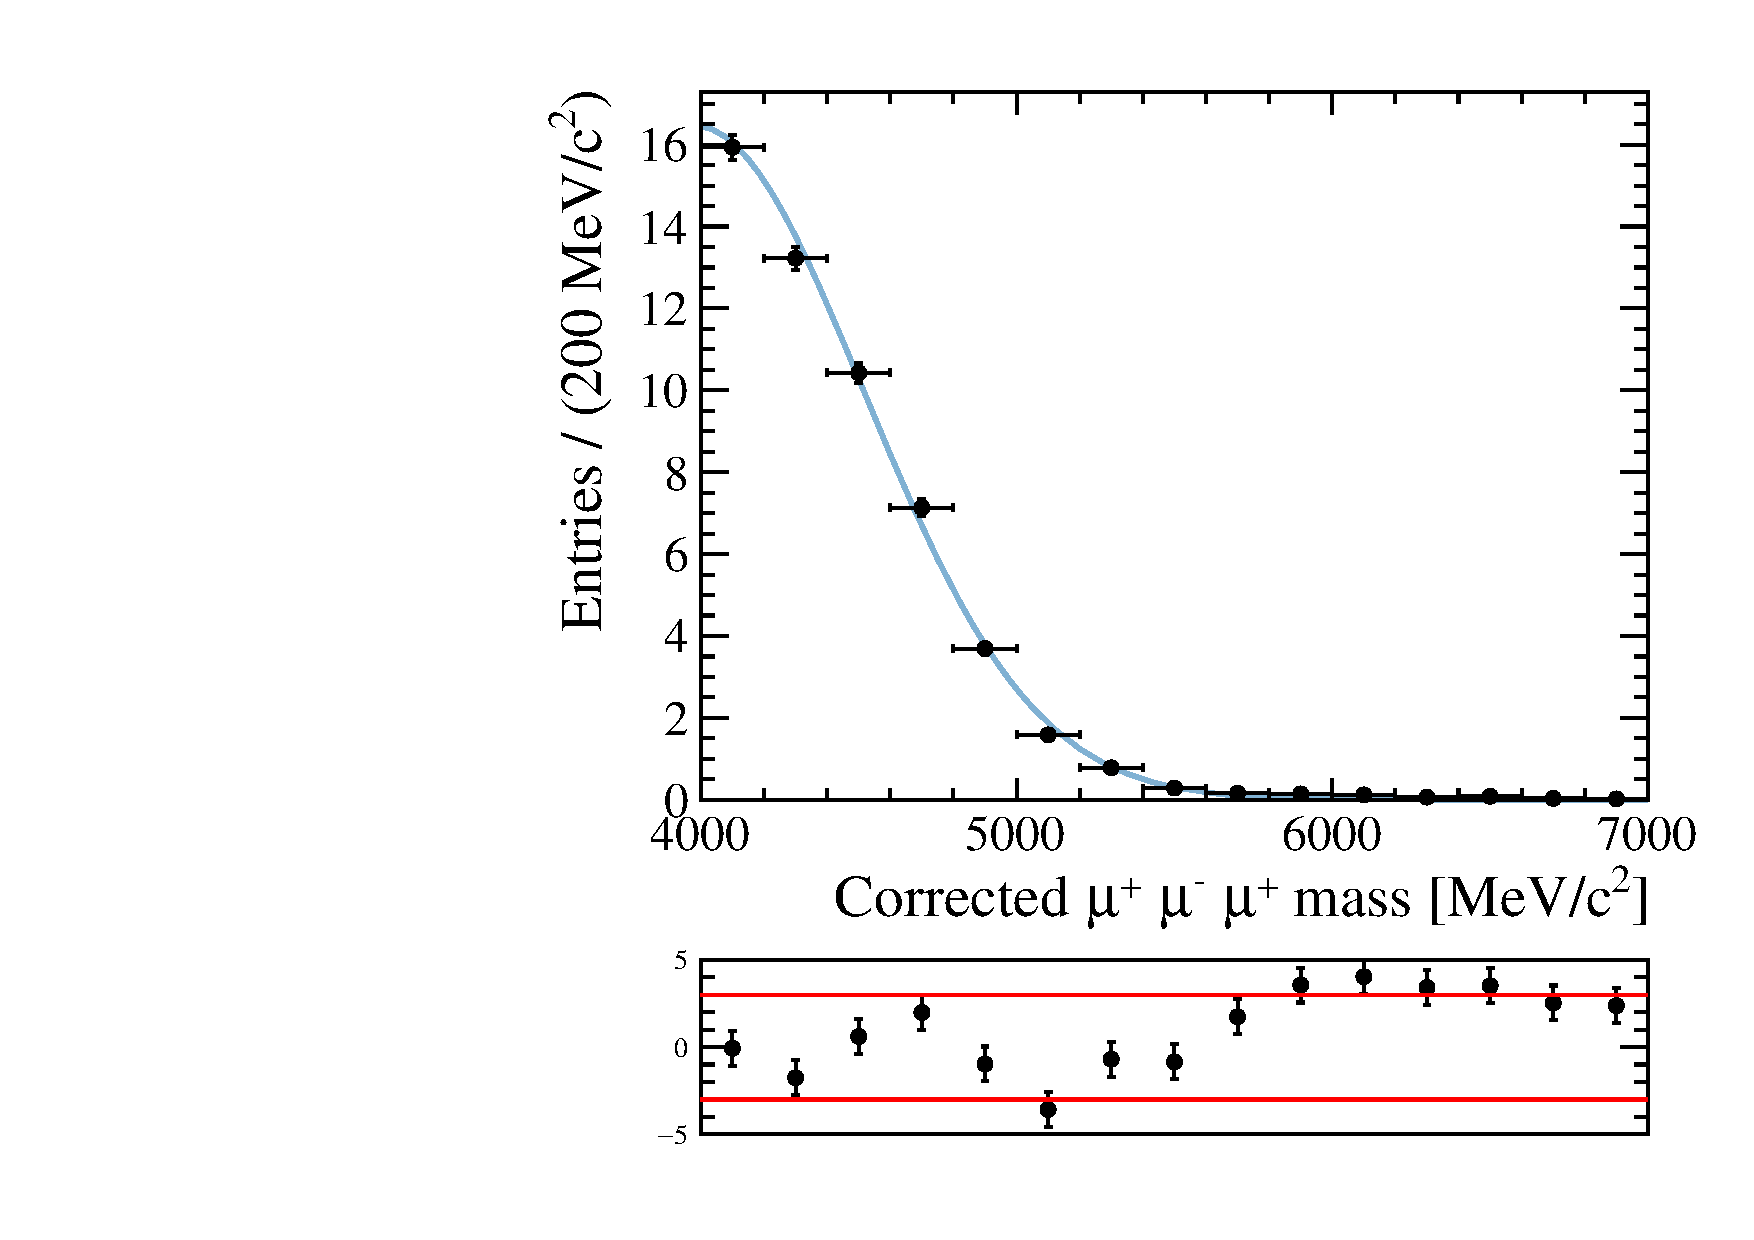
\includegraphics[width=0.5\linewidth]{./sel/plotMisidFitPretty_Run1.pdf}\put(-50,133){(a)}
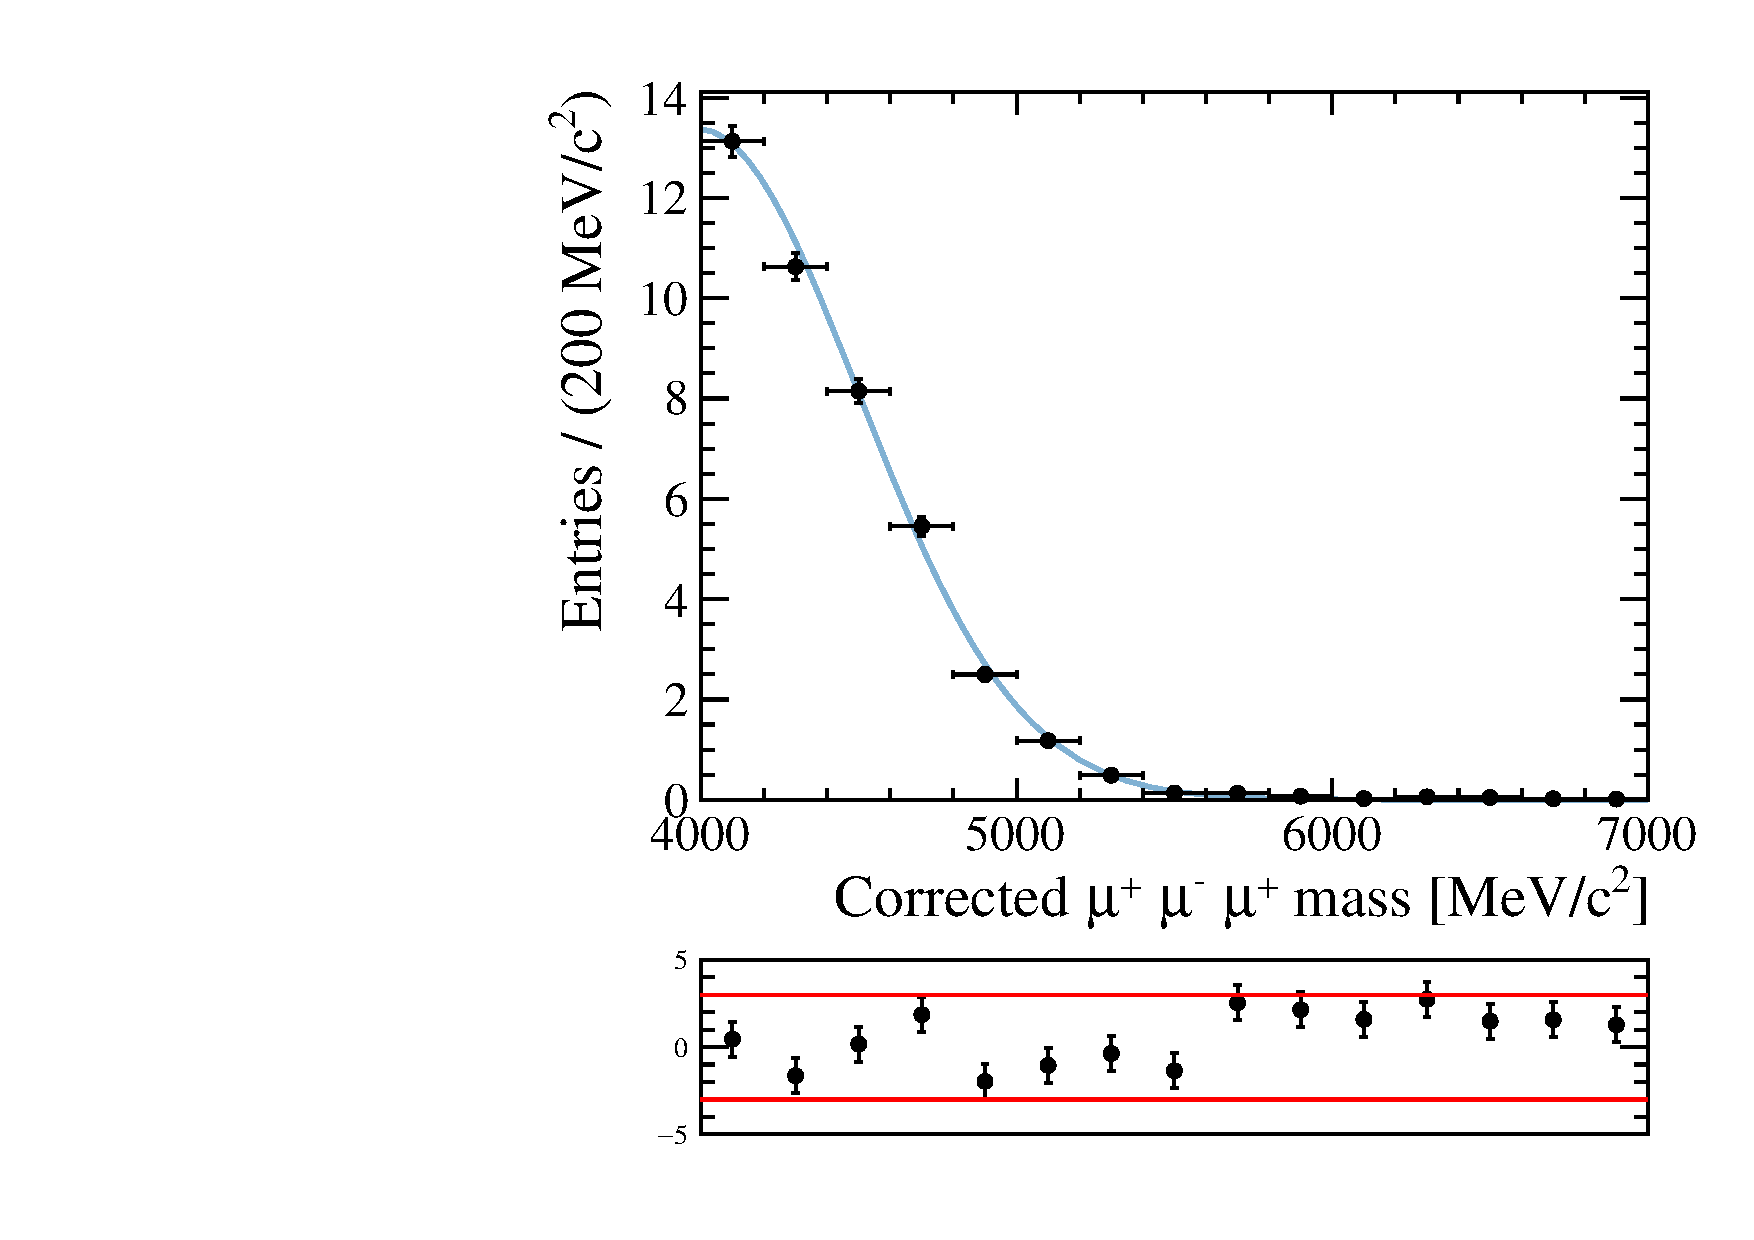
\includegraphics[width=0.5\linewidth]{./sel/plotMisidFitPretty_2016.pdf}\put(-50,133){(b)}
\caption{(a) Run1 (b) 2016 binned $\chi^{2}$ fit to misID sample yielding estimates for the number of background events.}
%\vspace*{-1.0cm}
\label{fig:beforemisiddatafit}
\end{figure}



The misID background can proceed also through combination with a random muon and hence by applying the combinatorial BDTs on the misID samples, this "combinatorial" component in the misID samples should be reduced and misID samples that are left should consist of true cascade decays. This can be seen in~\autoref{fig:combionmisid2016}.

\begin{figure}[ht]
\centering
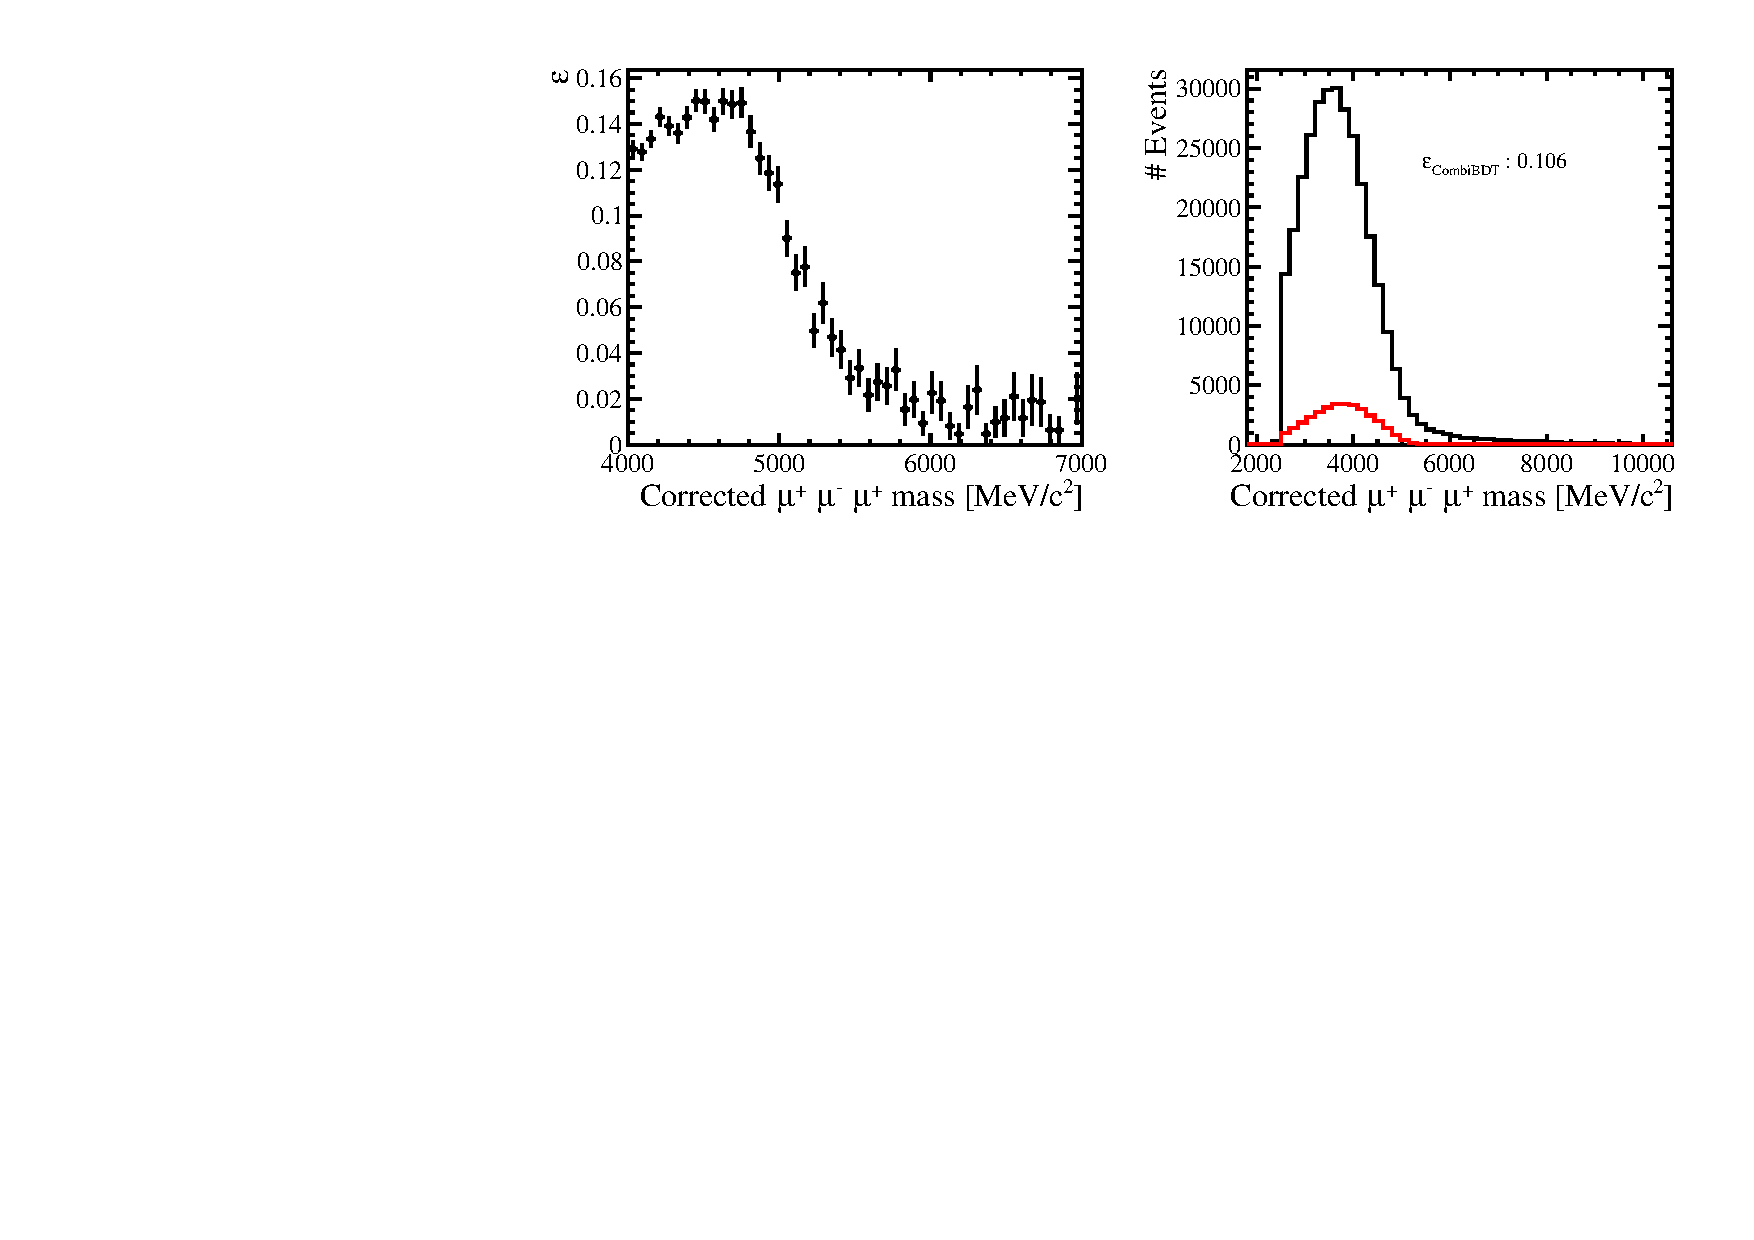
\includegraphics[width=0.9\linewidth]{./sel/CutEfficiency_Bplus_Corrected_MassMisid_nice.pdf}\put(-300,133){(a)}\put(-50,133){(b)}
\caption{(a) The efficiency of applying 2016 combinatorial BDT at optimal working point on the 2016 SS misID sample. It can be seen that (b) combinatorial component of the misID sample has been significantly reduced, where red curve is the distribution after applying the cut.}
\label{fig:combionmisid2016}
\end{figure}

The most powerful variables that distinguish the signal from misID background are the kinematic properties of the misidentified muon, namely $p_{T}$, $p$ and \gls{minipchi2}. Misidentified muons tend to be softer than in the signal case as they come from cascades via $D^{0}$ and its excited states. The \gls{minipchi2} distribution will be different as the misidentified muon can proceed $D^{0}$, rather than directly from the $B$. The kinematic distributions are also different for the two real muons between signal and misID background samples. The real muon that has the same charge as $B$ tends to be softer for the signal case whereas the real muon that has opposite charge proceeding via $D$ will be harder, as seen~\autoref{fig:dismisif}.


\begin{figure}[ht]
\centering
	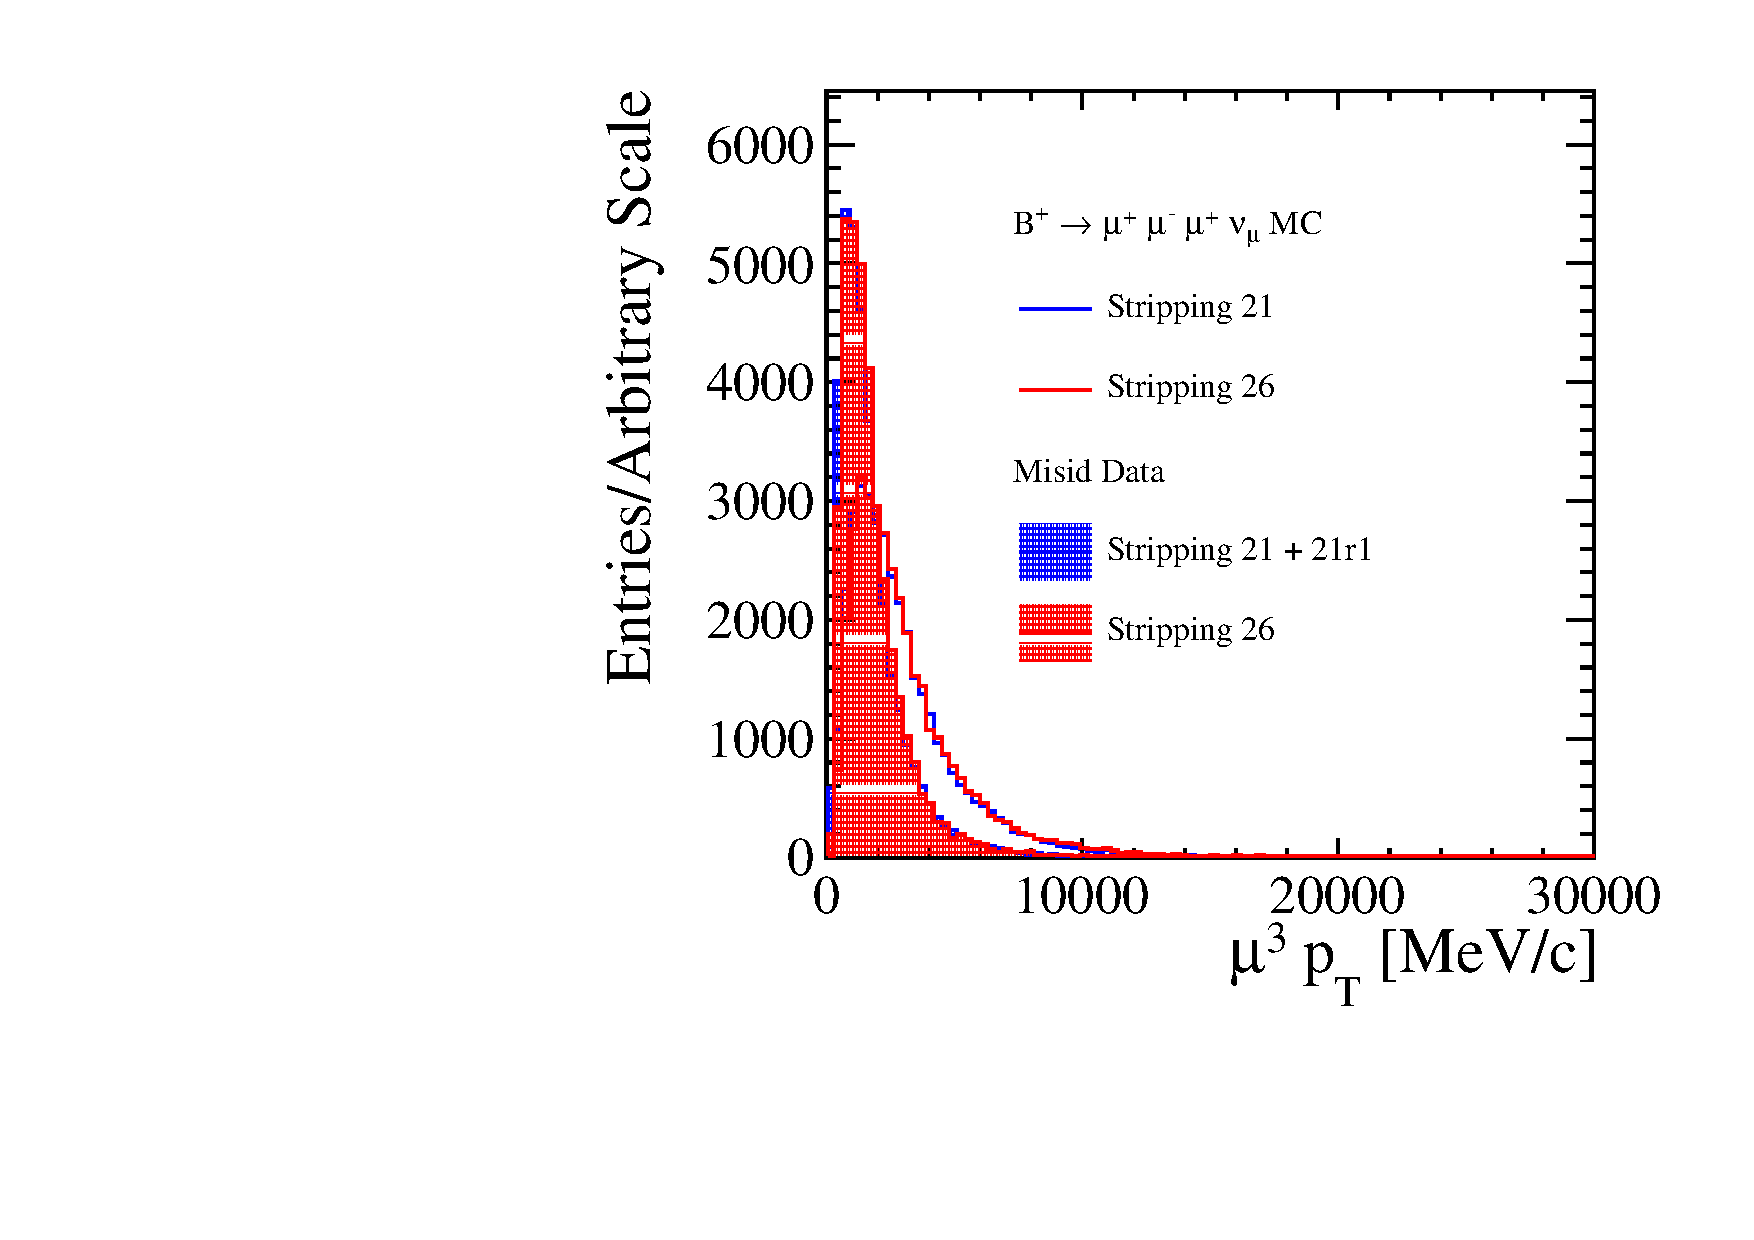
\includegraphics[width=0.5\linewidth]{./sel/misid/plotvariablemu3_PTNICEDISMIX.pdf}%
	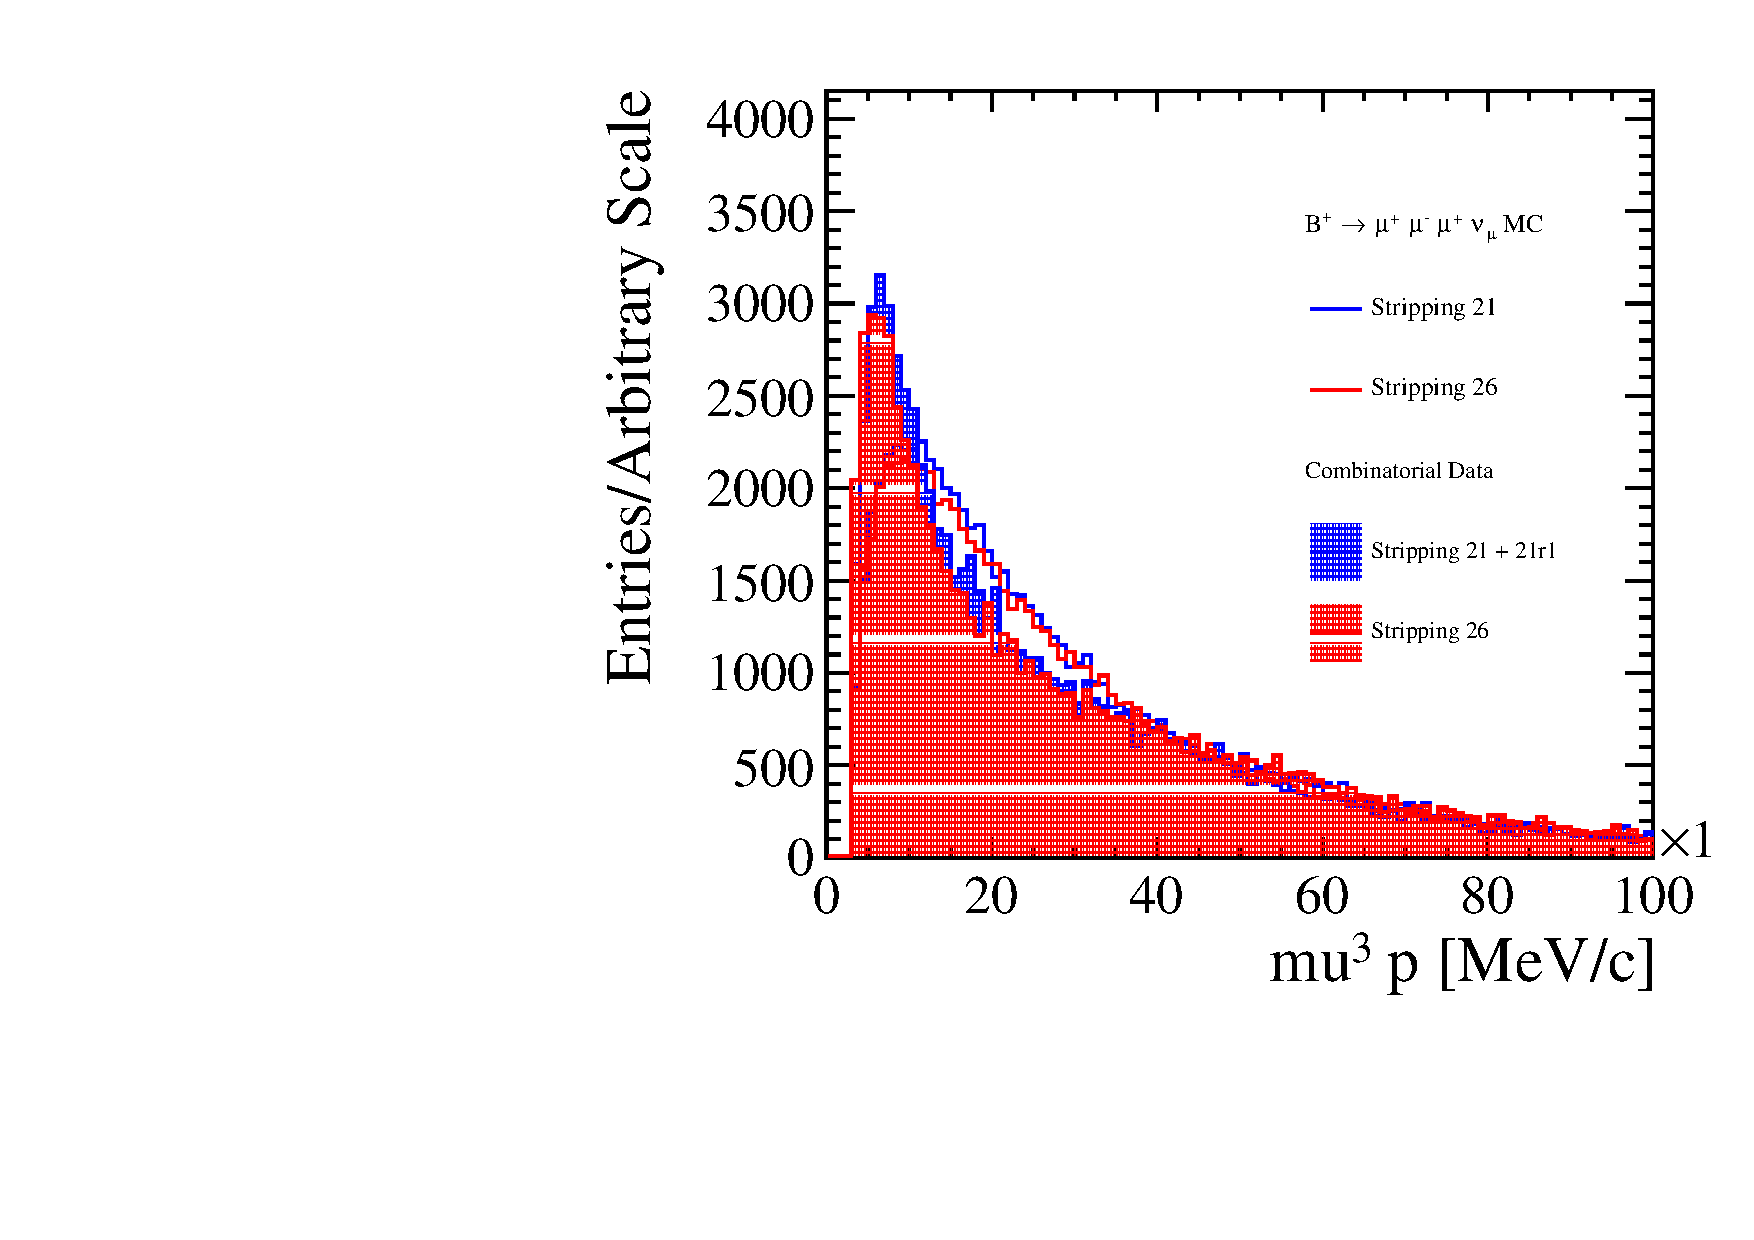
\includegraphics[width=0.5\linewidth]{./sel/misid/plotvariablemu3_PNICEDISMIX.pdf}%
	\newline
	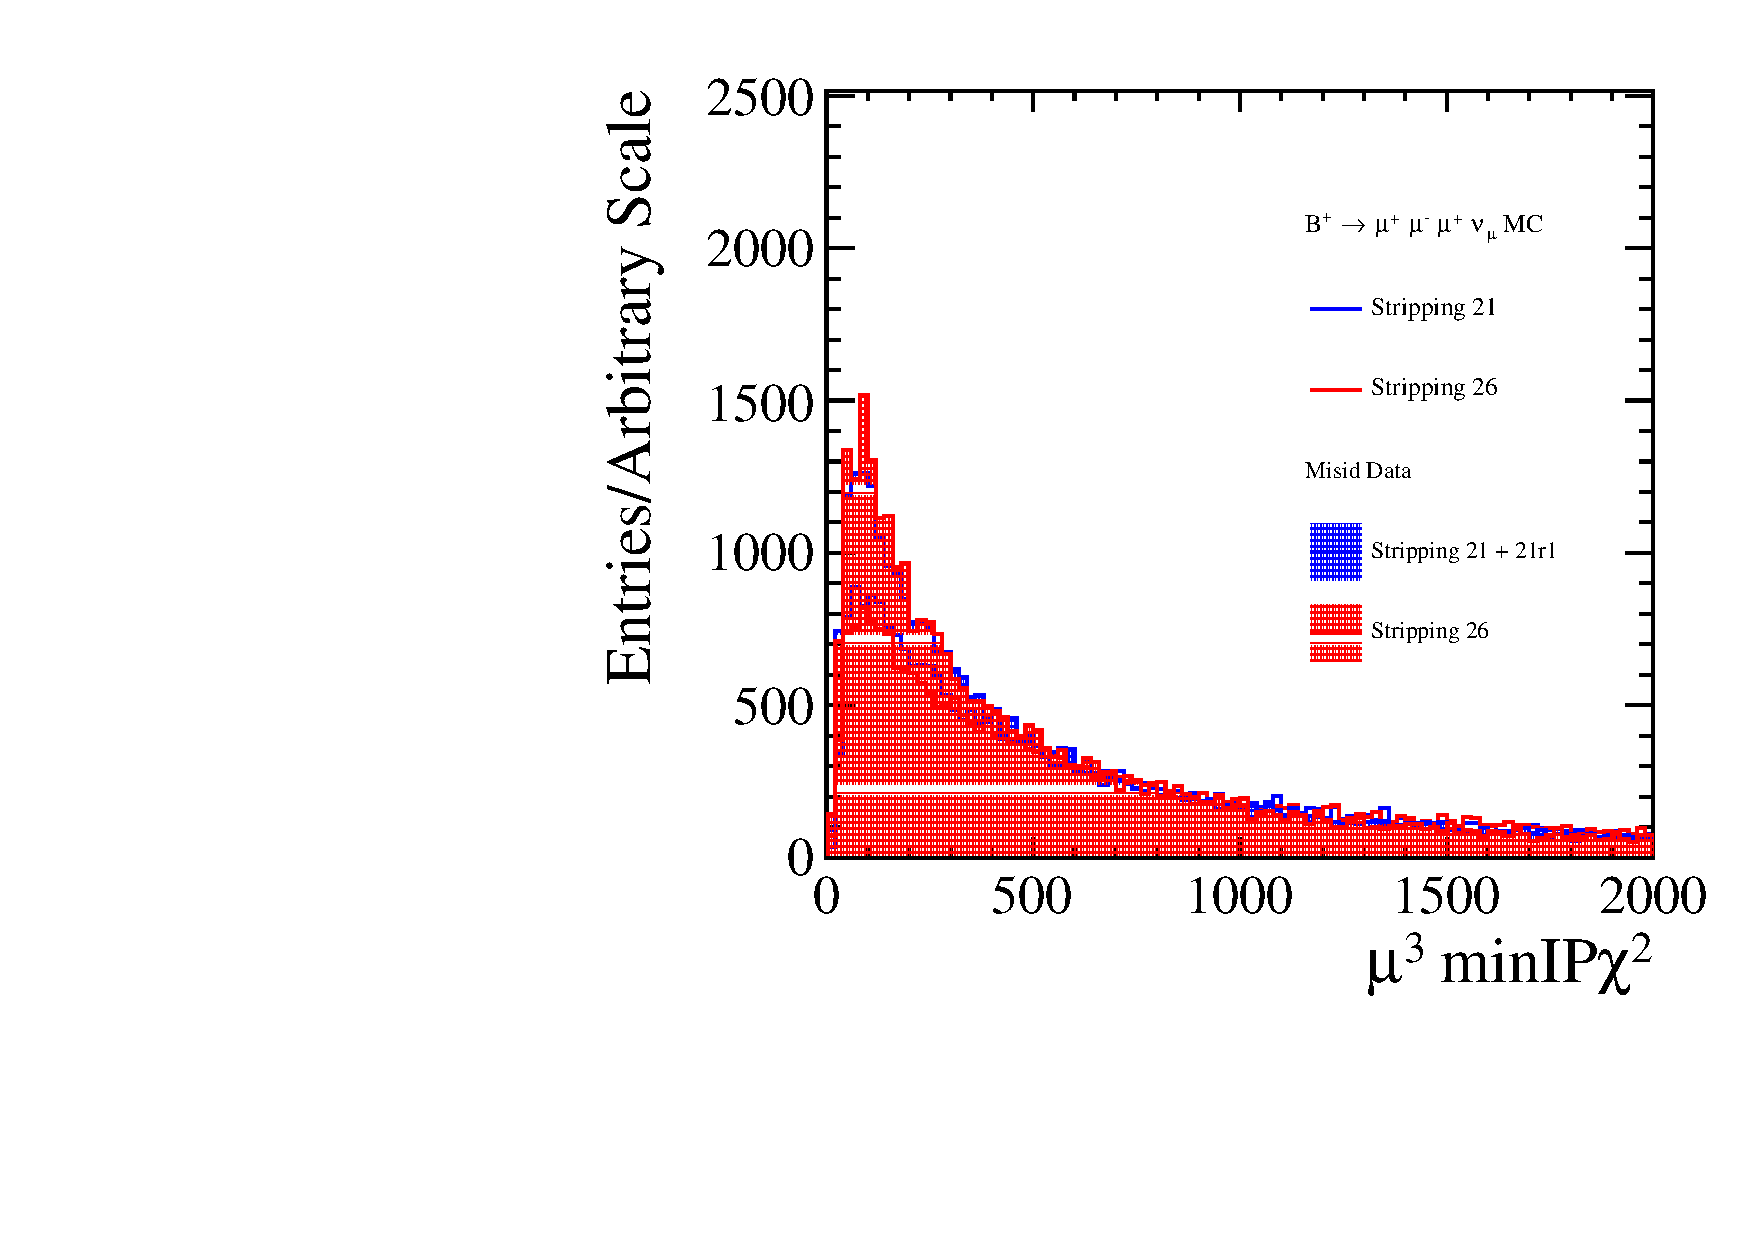
\includegraphics[width=0.5\linewidth]{./sel/misid/plotvariablemu3_MINIPCHI2NICEDISMIX.pdf}%
	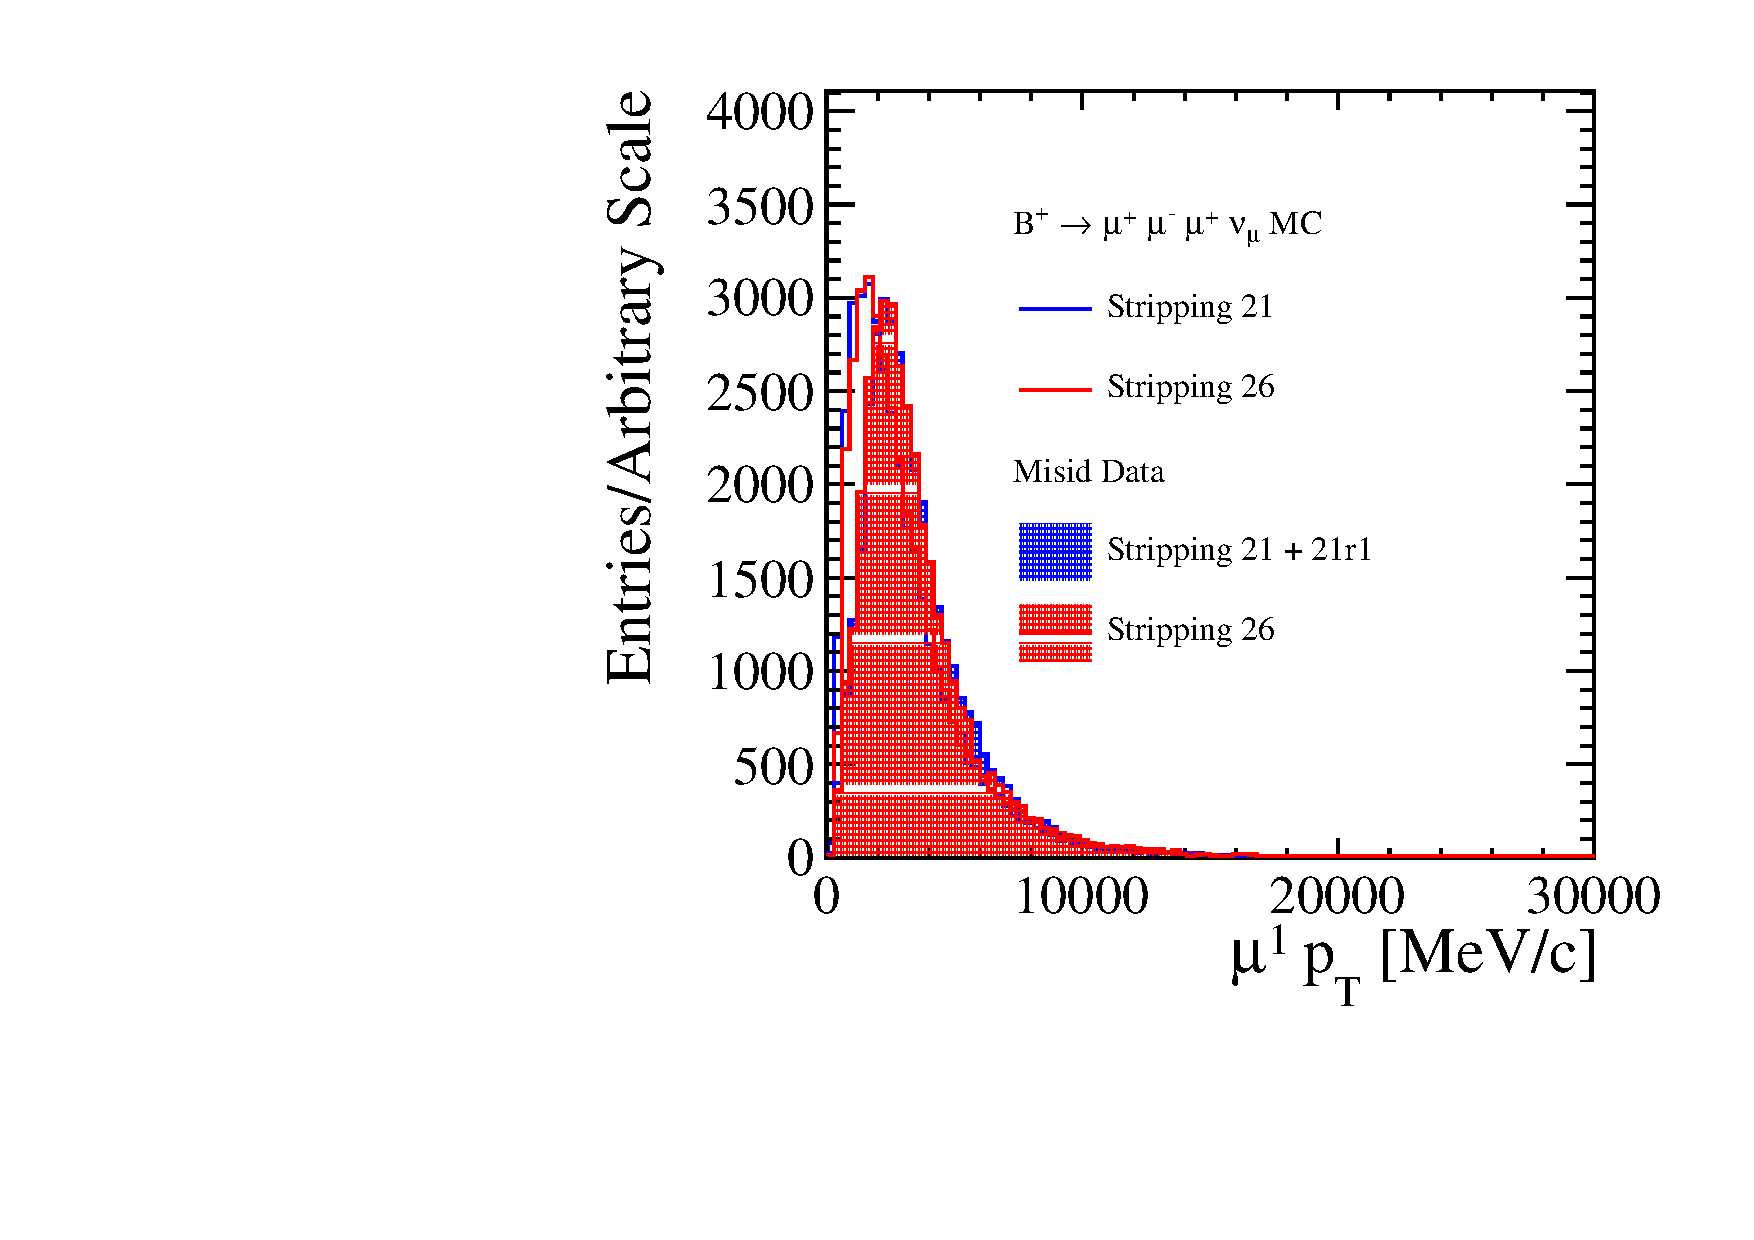
\includegraphics[width=0.5\linewidth]{./sel/misid/plotvariablemu1_PTNICEDISMIX.pdf}%
        \newline
	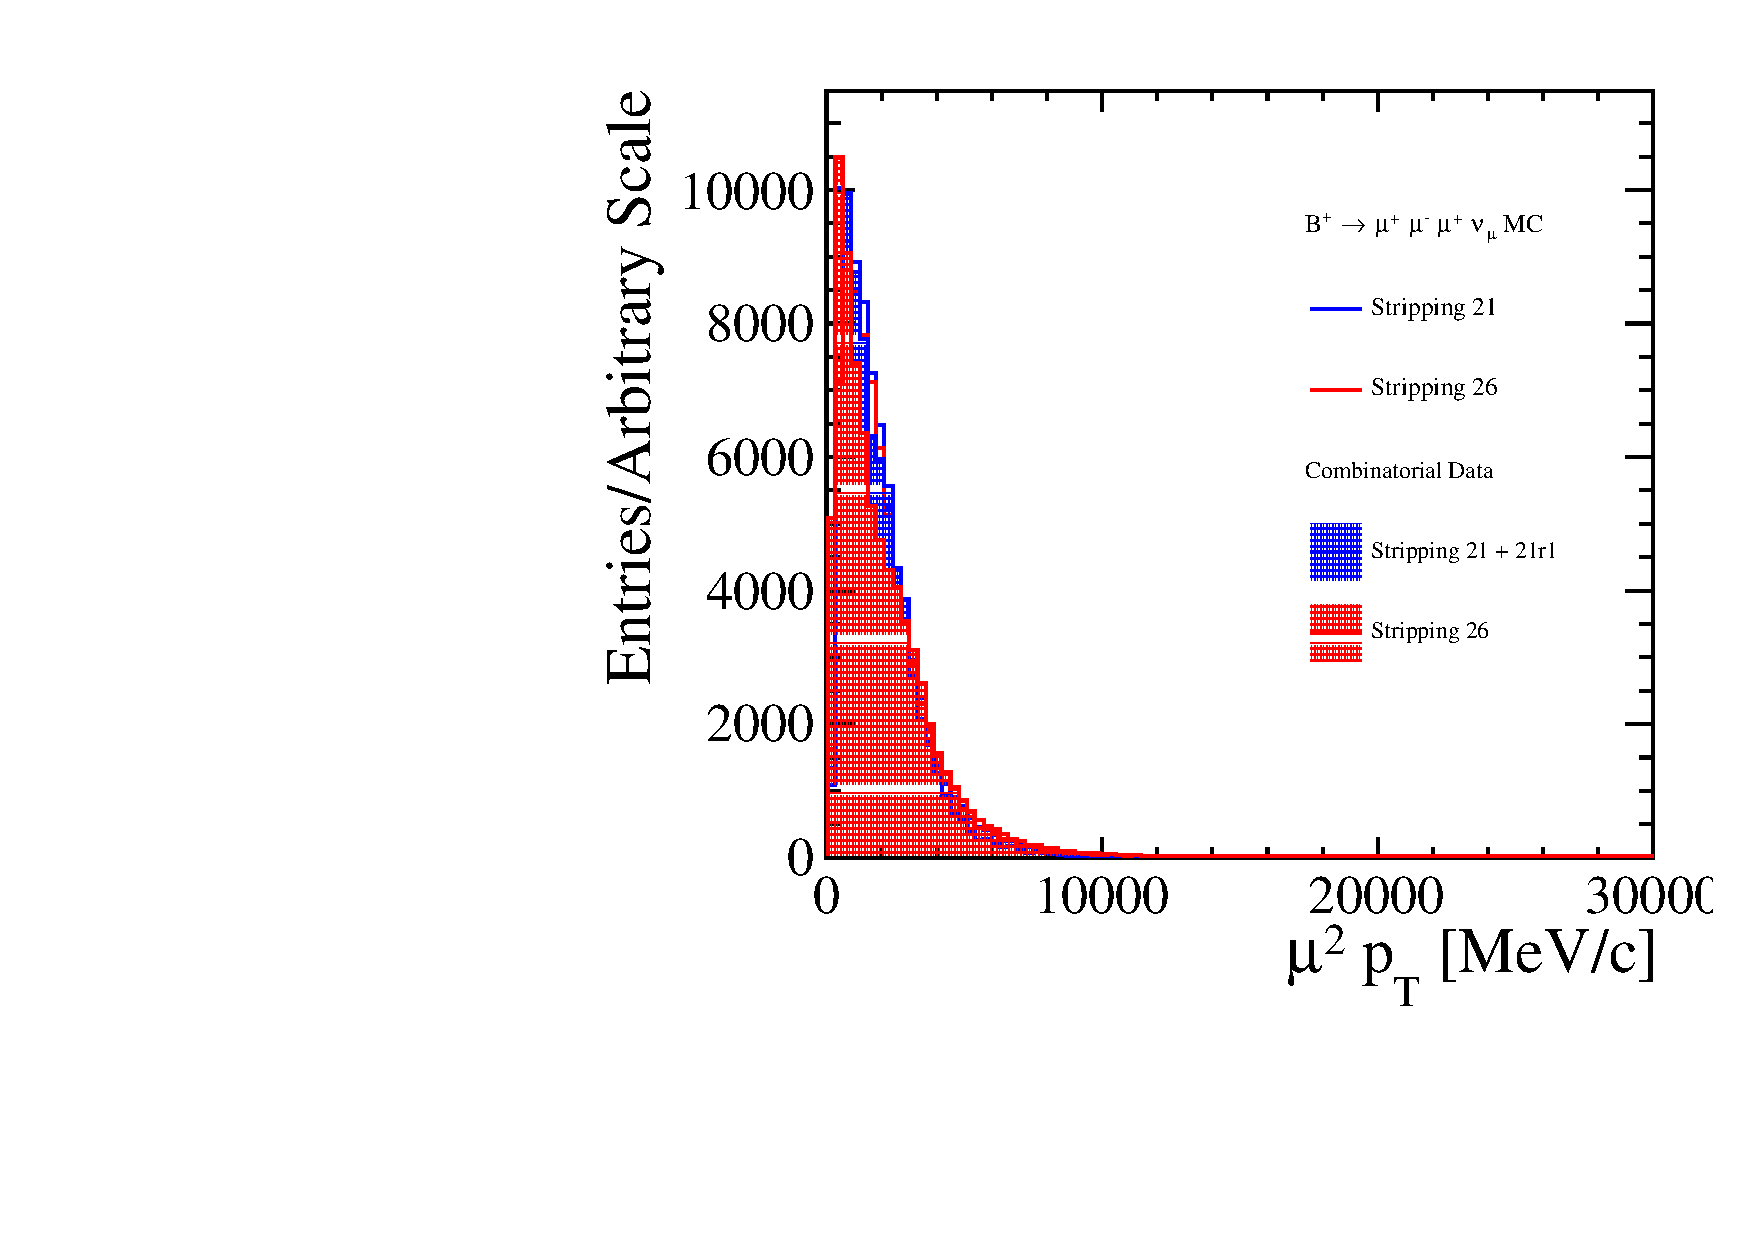
\includegraphics[width=0.5\linewidth]{./sel/misid/plotvariablemu2_PTNICEDISMIX.pdf}%
	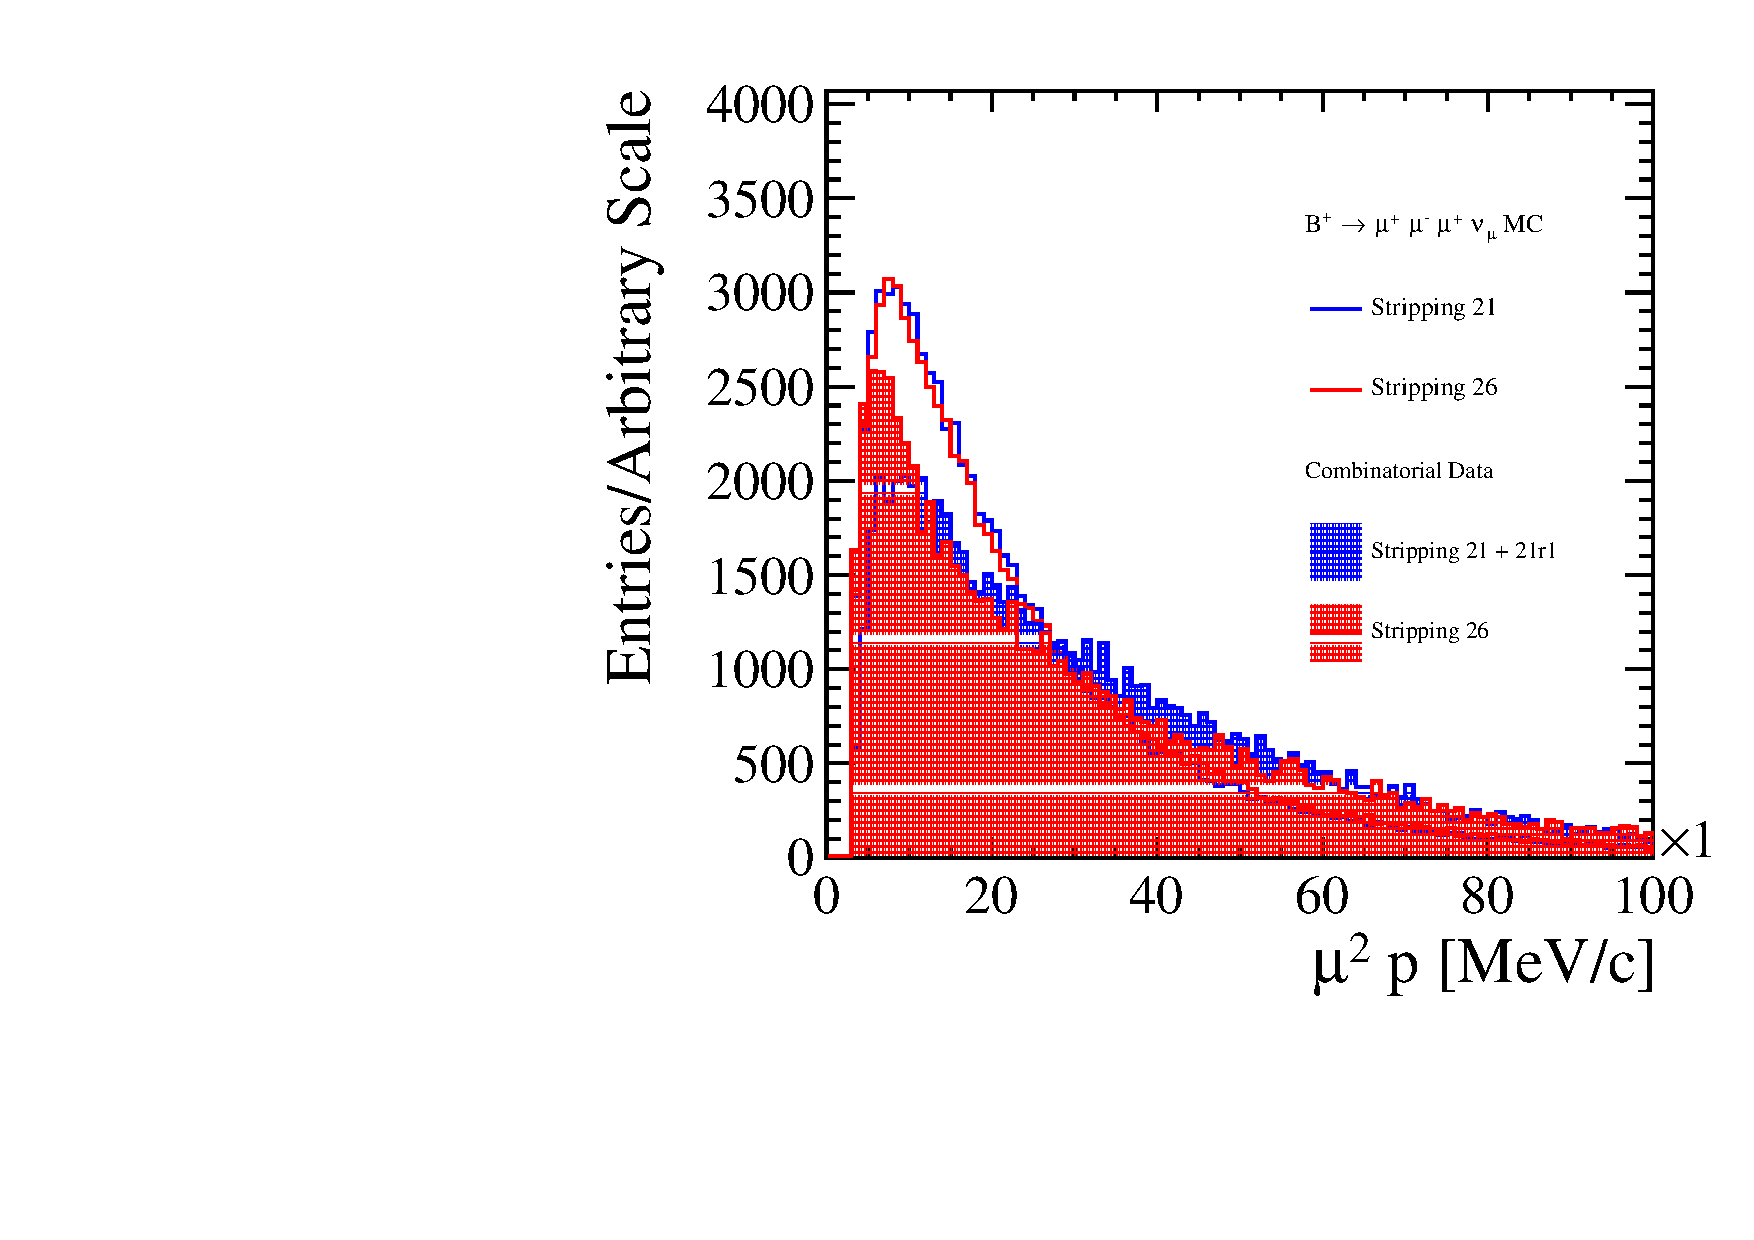
\includegraphics[width=0.5\linewidth]{./sel/misid/plotvariablemu2_PNICEDISMIX.pdf}%
	\caption{The variables with the most discriminative power for both misid Run \Rn{1} and \Rn{2} BDT, mostly kinematic properties of different muons.}
\label{fig:dismisif}
\end{figure}

\subsection{Fitting Region Selection}
\label{fittingsel}

Because the signal mass distribution is expected to be in a more narrow window around the $B^{+}$ peak in corrected mass and the exponential description of combinatorial background is not correct below $4000$ \mevcc, as will be shown in~\autoref{combiback}, the fitting region selection in which the measurement will be made is $4000$ \mevcc $<M_{B_{corr}}<$ $7000$ \mevcc.

\subsection{Further \gls{PID} Selection}
\label{furtherpid}
After classifiers to reduce combinatorial and misID backgrounds are trained and applied and the fitting region is defined, further \gls{PID} selection is performed. This can be done as the preselection had relatively loose $\rm{DLL}$ requirements and hence it is possible to improve the performance by using cuts on additional \gls{PID} variables. In the optimisation procedure, different hypotheses were tested, such as cuts on \texttt{Probnnmu}, \texttt{Probnnpi}, and \texttt{ProbnnK} variables and their combinations. The optimisation was performed in such a way as to optimize Punzi \texttt{FOM} with $\sigma=3$ in a blinded signal region, by performing the full blinded data fit (more information will be given in~\autoref{blindeddatafit}), but with fits to Run \Rn{1} and Run \Rn{2} data separately.


%In 2016, misID templates above 5800 \mevcc are not populated. Hence final 6 bins of corrected mass ($5800 \mevcc -7000 \mevcc$) are merged into 1. 
For each PID hypothesis, the Punzi \texttt{FOM} was calculated. In both cases, in \Rn{1} and \Rn{2} \texttt{Probnnmu} $>$ 0.35 yielded the highest Punzi \texttt{FOM}.



%\section{Multiple Candidates}
%After all the selection performed, in blinded datasets, $M_{B_{corr}}<4500$ \mevcc and $M_{B_{corr}}>5500$ \mevcc there is very few candidates left: $683$ in Run \Rn{1} and $505$ in \Rn{2} and no multiple candidates are seen.




\section{Normalisation channel}
\label{nchannel}
The normalisation channel used in this analysis is $ B^{+} \rightarrow (J/\psi \rightarrow \mu^{+} \mu^{-}) K^{+}$
as it is clean, well understood, and well-populated channel that is similar to signal. This means that many systematic uncertainties will cancel. Normalising the signal decay to this decay also means that absolute efficiencies, luminosity, the b-quark cross-section or fragmentation fractions will be cancelled. With the same number of tracks, it will also give a small uncertainty in the tracking efficiency. There are, however, a few differences in the selection that need to be underlined.

Firstly, the preselection stream from which this sample is taken has different requirements seen in~\autoref{tab:stripcutsBnorm}. As compared to preselection of the signal channel shown in~\autoref{tab:stripcutsB}, this preselection is less tight. To unify and impose same kind of preselection so that the tracks chosen are of a good quality and away from \gls{PV}, the preselection for signal channel is applied on the top of the original preselection.


\begin{table}%[H]
\begin{center}
\begin{tabular}{l|c l }

    \toprule
     Candidate & Stripping Selection \\ \hline

	muon & $p_{T} >$ 500 \mev \\ 

	
	muon & DLLmu$ > 0$ & \rdelim\}{1}{1cm}[\ \gls{PID}] \\ \hline

	kaon & PT > 500 \mev \\ 
	kaon & \gls{trackchi2ndof}$ < 5$ \\
	kaon & $\rm{DLLK} > 0$ & \rdelim\}{1}{1cm}[\ \gls{PID}] \\ \hline

%	dimuon & DOCA $\chi^{2}$ < 20  \\ This one is not listed as the below one has stronger imposation
	dimuon & \gls{vertexchi2ndof} $< 16$ \\
	dimuon & $| M(\mu^{+},\mu^{-})\ -\ M_{PDG}(J/\psi)|\ <\ 80\ \mevcc$ \\ \hline

	combination & \gls{vertexchi2ndof} $< 10$ \\
	combination & $5150\ \mevcc\ <\ M_B\ <\ 5450\ \mevcc$ \\
	combination & $B$ lifetime > 0.2 ps \\ \bottomrule
     \end{tabular}

\end{center}
	\caption{Original preselection of events for normalisation channel for $B^{+} \rightarrow (J/\psi \rightarrow \mu^{+} \mu^{-}) K^{+}$ for Run \Rn{1} and Run \Rn{2}. }
\label{tab:stripcutsBnorm}
\end{table}


Secondly, this decay proceeds via the $J/\psi$ resonance and hence the $q^{2}$ veto for $J/\psi$ and $\Psi{(2S)}$, listed in~\autoref{tab:vetoes}, is not applied but rather reversed as seen in~\autoref{tab:stripcutsBnorm}. As the third particle is a kaon rather than muon, there is no explicit choice of $minq$ region.

And finally the kaon candidates are required to have \gls{PID} criteria consistent with being a kaon. In addition to the preselection already imposing $\rm{DLLK} > 0$,  $\rm{DLLp} - \rm{DLLK}< 5$ is required to make a distinction with protons. To assure that the kaon is not confused with the muon, \texttt{IsMuon==0.0} is imposed. But only kaon tracks, which have the properties that they could be within geometrical muon acceptance, \texttt{InMuonAcc==1.0}, are considered.  
%$\epsilon_{PID}$ is the efficiency of PID, that is taken from control data samples and then parametrically applied to simulation samples.


\section{Fractional Corrected Mass Error (FCME) Window Split}
\label{split}
In order to increase sensitivity, but not to decrease statistics as all the previous selection leads to a low-statistics regime, it was decided that the fitting procedure for the final fit will be in two bins of the estimated fractional corrected mass error (FCME), defined as
\begin{equation}
	\sigma_{\rm{\{lowFCME,highFCME\}}} = \frac{\delta}{M_{B_{corr}}},
\label{eq:fraccormerr}
\end{equation}


where $\delta$ is the corrected mass error. Because the corrected mass error has clear dependence on resolution (see ~\autoref{fig:resolution}), this split will divide the data into two bins of resolution increasing the sensitivity for observation.
\begin{figure}[H]
\centering
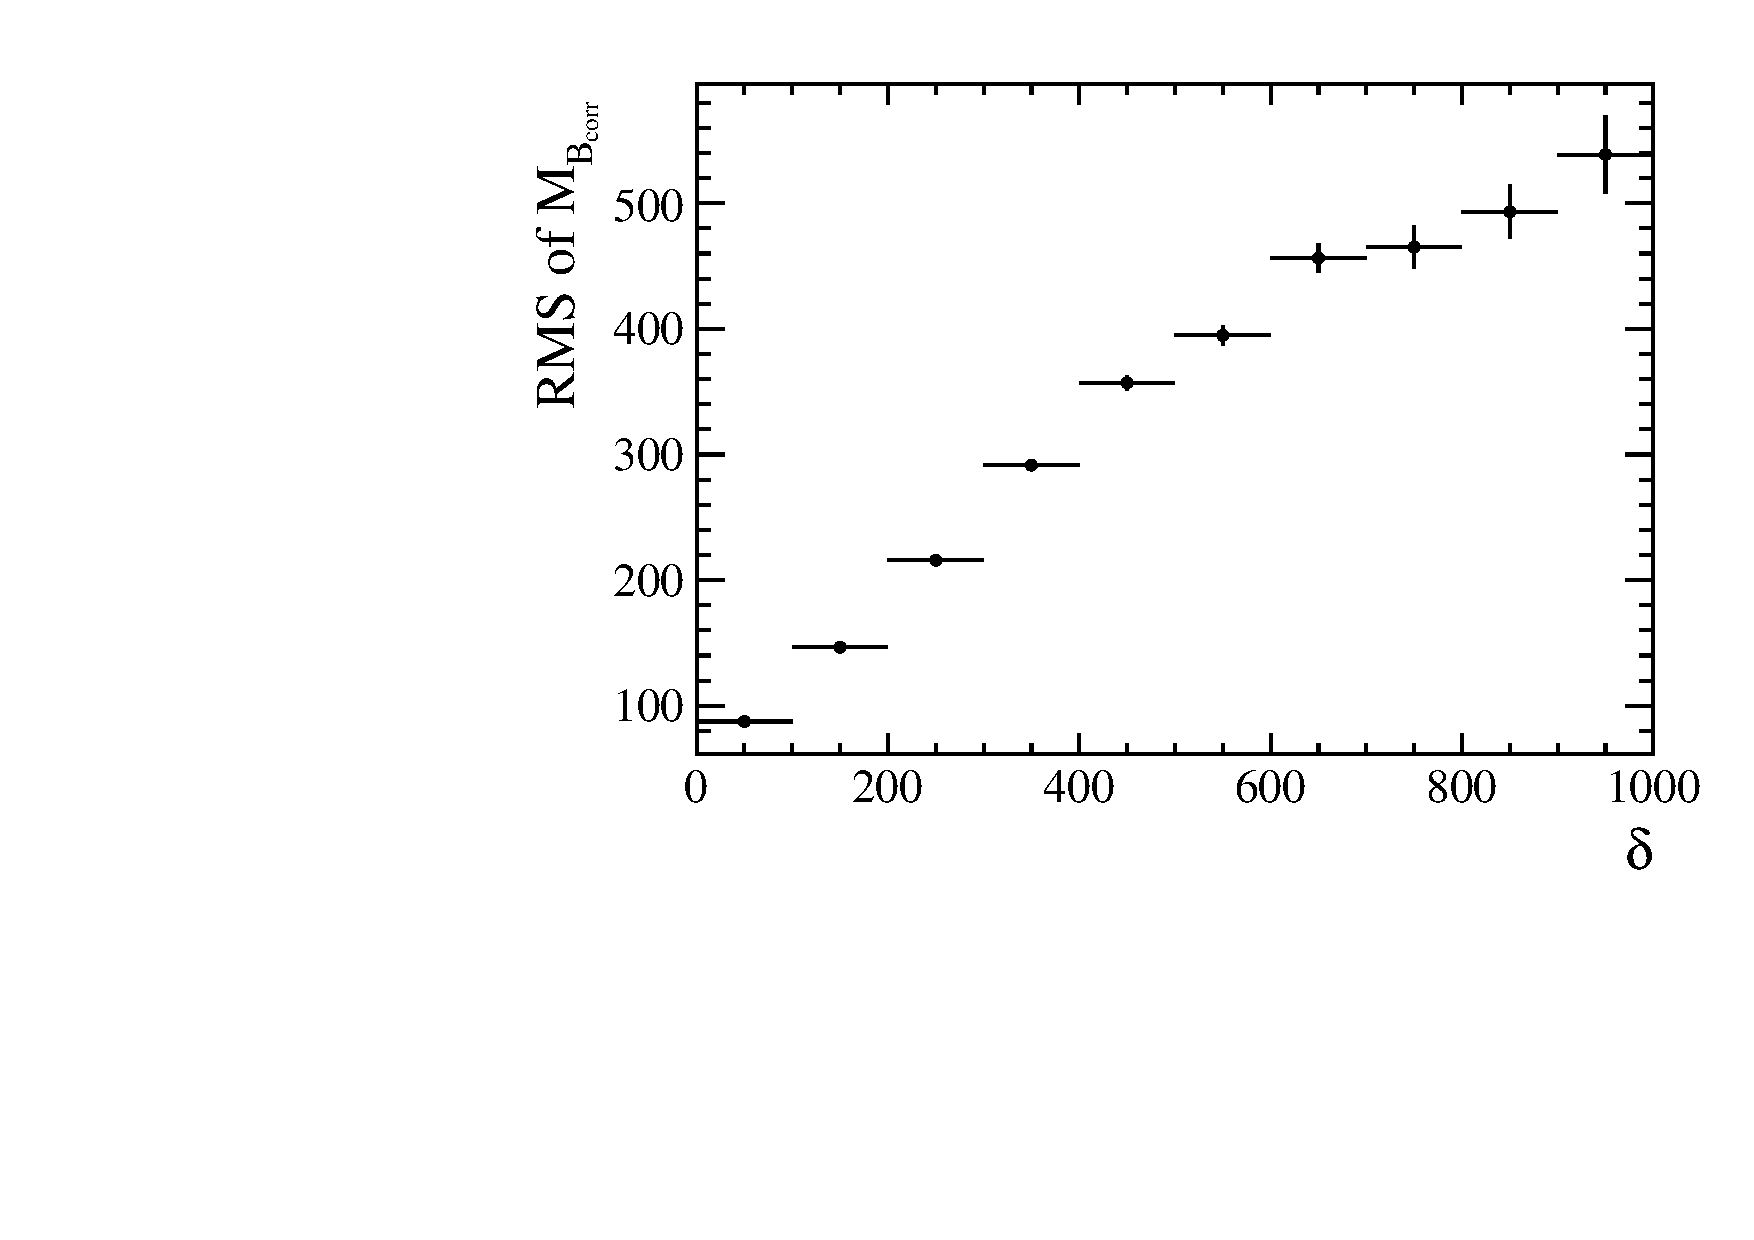
\includegraphics[width=0.5\linewidth]{sel/trial2012.pdf}\put(-100,133){(a)}
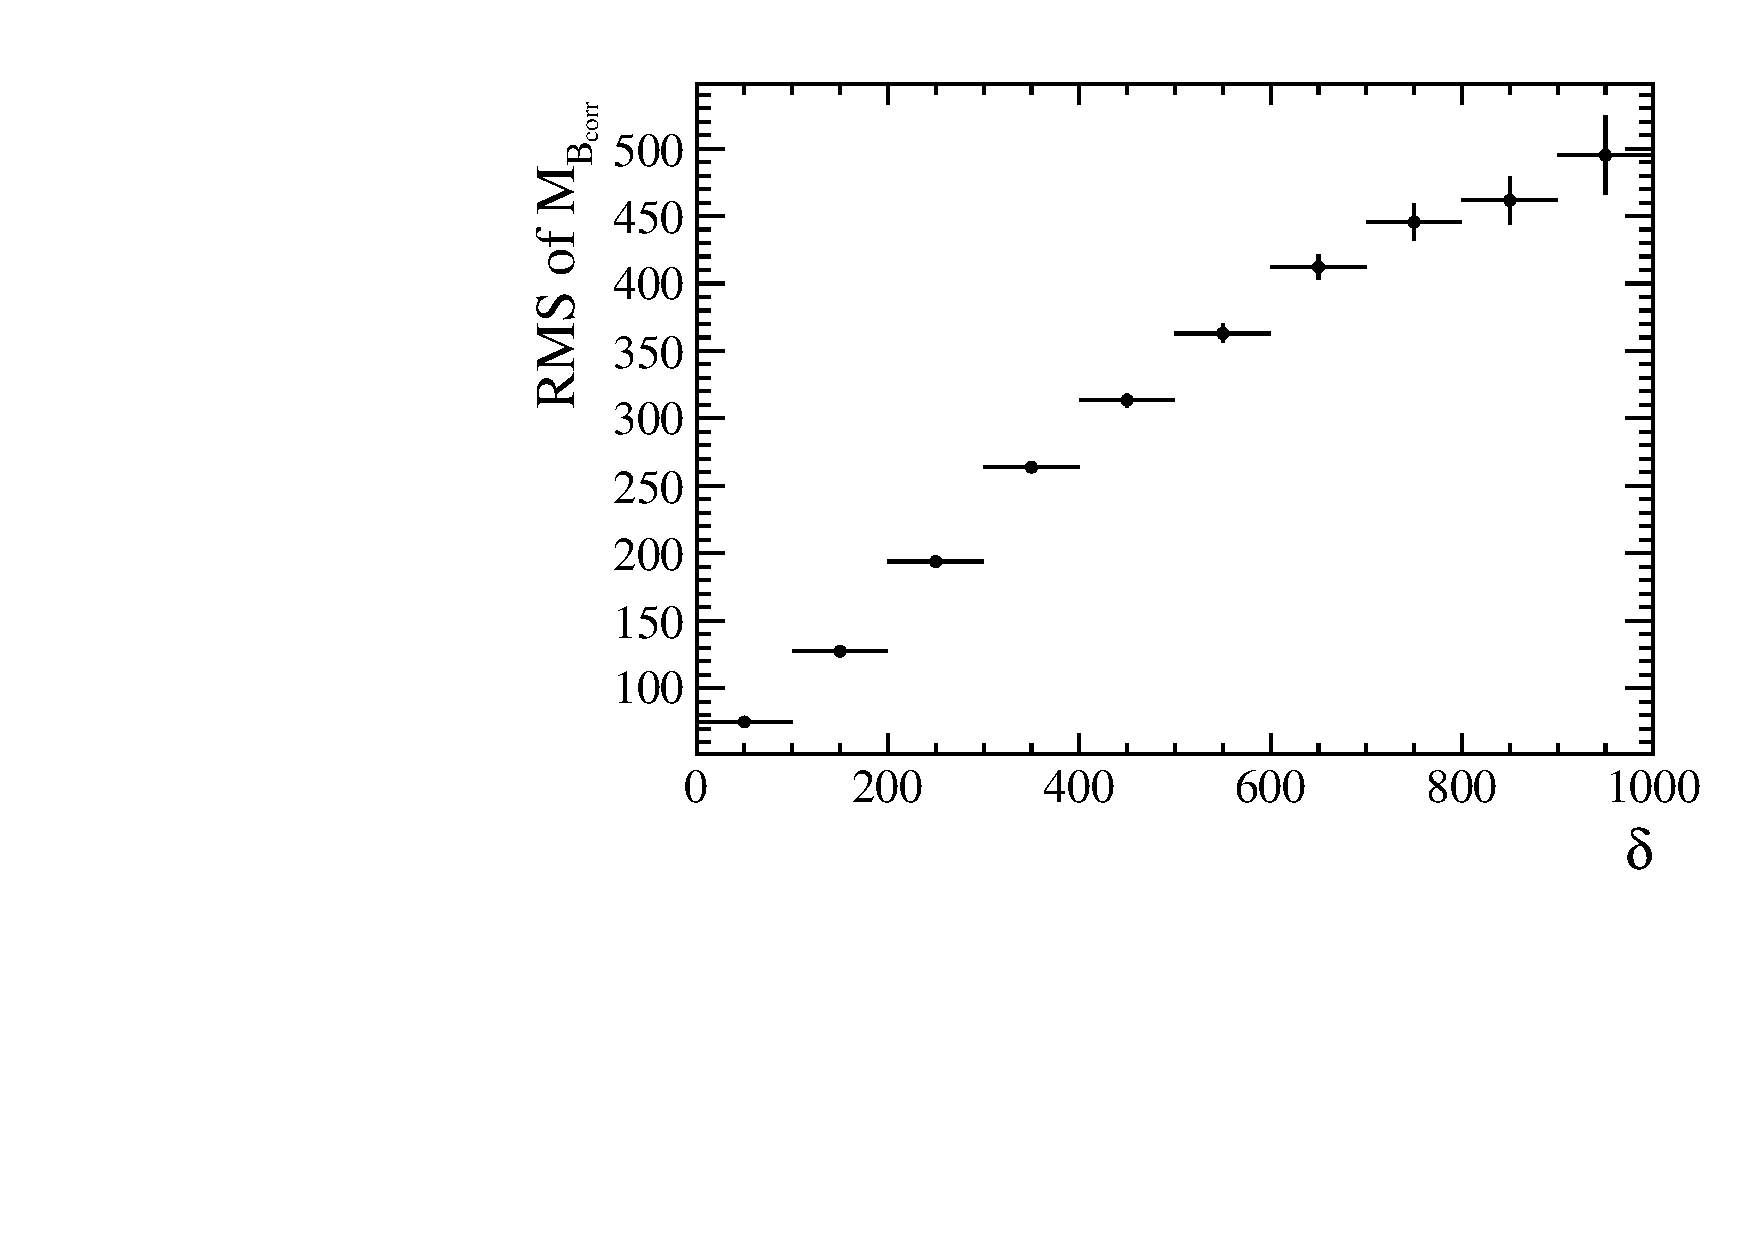
\includegraphics[width=0.5\linewidth]{sel/trial2016.pdf}\put(-100,133){(b)}
\caption{ (a) The resolution of 2012 signal simulation in bins of the estimated corrected mass error $\delta$. (b) The resolution of 2016 signal simulation in bins of corrected mass error $\delta$. }
\label{fig:resolution}
%\vspace*{-1.0cm}
\end{figure}

The split boundary was chosen in such a way as to keep $\sim50\%$ of signal in $\sigma_{\rm{lowFCME}}$ and $\sim50\%$ signal in high $\sigma_{\rm{highFCME}}$.
Numerically this corresponds to 

\begin{equation}
\sigma_{\rm{\{lowFCME,highFCME\}}}=
   \begin{dcases}
	   \sigma_{\rm{lowFCME}} &\text{if  }  \frac{\delta}{M_{B_{corr}}} < 0.0225,\\
	  \sigma_{\rm{highFCME}} &\text{if  }  \frac{\delta}{M_{B_{corr}}} > 0.0225. 
   \end{dcases}
\label{eq:impsplit}
\end{equation}

However, in order to look at the consistency of this two bin strategy also one bin of fractional corrected mass error strategy is performed and will be denoted as $\sigma_{\rm{NOFCME}}$.
